\documentclass[twoside]{book}

% Packages required by doxygen
\usepackage{fixltx2e}
\usepackage{calc}
\usepackage{doxygen}
\usepackage{graphicx}
\usepackage[utf8]{inputenc}
\usepackage{makeidx}
\usepackage{multicol}
\usepackage{multirow}
\PassOptionsToPackage{warn}{textcomp}
\usepackage{textcomp}
\usepackage[nointegrals]{wasysym}
\usepackage[table]{xcolor}

% Font selection
\usepackage[T1]{fontenc}
\usepackage{mathptmx}
\usepackage[scaled=.90]{helvet}
\usepackage{courier}
\usepackage{amssymb}
\usepackage{sectsty}
\renewcommand{\familydefault}{\sfdefault}
\allsectionsfont{%
  \fontseries{bc}\selectfont%
  \color{darkgray}%
}
\renewcommand{\DoxyLabelFont}{%
  \fontseries{bc}\selectfont%
  \color{darkgray}%
}
\newcommand{\+}{\discretionary{\mbox{\scriptsize$\hookleftarrow$}}{}{}}

% Page & text layout
\usepackage{geometry}
\geometry{%
  a4paper,%
  top=2.5cm,%
  bottom=2.5cm,%
  left=2.5cm,%
  right=2.5cm%
}
\tolerance=750
\hfuzz=15pt
\hbadness=750
\setlength{\emergencystretch}{15pt}
\setlength{\parindent}{0cm}
\setlength{\parskip}{0.2cm}
\makeatletter
\renewcommand{\paragraph}{%
  \@startsection{paragraph}{4}{0ex}{-1.0ex}{1.0ex}{%
    \normalfont\normalsize\bfseries\SS@parafont%
  }%
}
\renewcommand{\subparagraph}{%
  \@startsection{subparagraph}{5}{0ex}{-1.0ex}{1.0ex}{%
    \normalfont\normalsize\bfseries\SS@subparafont%
  }%
}
\makeatother

% Headers & footers
\usepackage{fancyhdr}
\pagestyle{fancyplain}
\fancyhead[LE]{\fancyplain{}{\bfseries\thepage}}
\fancyhead[CE]{\fancyplain{}{}}
\fancyhead[RE]{\fancyplain{}{\bfseries\leftmark}}
\fancyhead[LO]{\fancyplain{}{\bfseries\rightmark}}
\fancyhead[CO]{\fancyplain{}{}}
\fancyhead[RO]{\fancyplain{}{\bfseries\thepage}}
\fancyfoot[LE]{\fancyplain{}{}}
\fancyfoot[CE]{\fancyplain{}{}}
\fancyfoot[RE]{\fancyplain{}{\bfseries\scriptsize Generated on Fri Dec 2 2016 21\+:55\+:15 for Tomada\+Pic\+Low\+Power by Doxygen }}
\fancyfoot[LO]{\fancyplain{}{\bfseries\scriptsize Generated on Fri Dec 2 2016 21\+:55\+:15 for Tomada\+Pic\+Low\+Power by Doxygen }}
\fancyfoot[CO]{\fancyplain{}{}}
\fancyfoot[RO]{\fancyplain{}{}}
\renewcommand{\footrulewidth}{0.4pt}
\renewcommand{\chaptermark}[1]{%
  \markboth{#1}{}%
}
\renewcommand{\sectionmark}[1]{%
  \markright{\thesection\ #1}%
}

% Indices & bibliography
\usepackage{natbib}
\usepackage[titles]{tocloft}
\setcounter{tocdepth}{3}
\setcounter{secnumdepth}{5}
\makeindex

% Hyperlinks (required, but should be loaded last)
\usepackage{ifpdf}
\ifpdf
  \usepackage[pdftex,pagebackref=true]{hyperref}
\else
  \usepackage[ps2pdf,pagebackref=true]{hyperref}
\fi
\hypersetup{%
  colorlinks=true,%
  linkcolor=blue,%
  citecolor=blue,%
  unicode%
}

% Custom commands
\newcommand{\clearemptydoublepage}{%
  \newpage{\pagestyle{empty}\cleardoublepage}%
}


%===== C O N T E N T S =====

\begin{document}

% Titlepage & ToC
\hypersetup{pageanchor=false,
             bookmarks=true,
             bookmarksnumbered=true,
             pdfencoding=unicode
            }
\pagenumbering{roman}
\begin{titlepage}
\vspace*{7cm}
\begin{center}%
{\Large Tomada\+Pic\+Low\+Power }\\
\vspace*{1cm}
{\large Generated by Doxygen 1.8.7}\\
\vspace*{0.5cm}
{\small Fri Dec 2 2016 21:55:15}\\
\end{center}
\end{titlepage}
\clearemptydoublepage
\tableofcontents
\clearemptydoublepage
\pagenumbering{arabic}
\hypersetup{pageanchor=true}

%--- Begin generated contents ---
\chapter{Todo List}
\label{todo}
\hypertarget{todo}{}

\begin{DoxyRefList}
\item[\label{todo__todo000001}%
\hypertarget{todo__todo000001}{}%
Member \hyperlink{analog_8h_aaac550cf000789bda83df7d9e151e8a4}{analog\+\_\+channel\+\_\+select\+\_\+t} ]Por hora, apenas o canal 0 foi implementado. Ver a necessidade de utilizar os outros.  
\item[\label{todo__todo000001}%
\hypertarget{todo__todo000001}{}%
Member \hyperlink{analog_8h_aaac550cf000789bda83df7d9e151e8a4}{analog\+\_\+channel\+\_\+select\+\_\+t} ]Por hora, apenas o canal 0 foi implementado. Ver a necessidade de utilizar os outros.  
\item[\label{todo__todo000004}%
\hypertarget{todo__todo000004}{}%
Member \hyperlink{usart_8h_a8016e6fb6f0a421fb1622403ccf7b16a}{usart\+\_\+receive\+\_\+interrupt\+\_\+isr} ()]Transformar em uma macro depois.  
\item[\label{todo__todo000002}%
\hypertarget{todo__todo000002}{}%
Member \hyperlink{usart_8h_a8a68523fcfebe109df61258219ae9688}{usart\+\_\+start} (usart\+\_\+sync\+\_\+mode\+\_\+t usart\+\_\+sync\+\_\+mode, uint32\+\_\+t baud\+\_\+rate)]Implementar modo sincrono!  
\item[\label{todo__todo000003}%
\hypertarget{todo__todo000003}{}%
Member \hyperlink{usart_8h_a0f565c4ece40219cd8e0499edb19f600}{usart\+\_\+transmite\+\_\+interrupt\+\_\+isr} ()]Transformar em uma macro depois. 
\end{DoxyRefList}
\chapter{File Index}
\section{File List}
Here is a list of all files with brief descriptions\+:\begin{DoxyCompactList}
\item\contentsline{section}{\hyperlink{analog_8c}{analog.\+c} }{\pageref{analog_8c}}{}
\item\contentsline{section}{\hyperlink{analog_8h}{analog.\+h} }{\pageref{analog_8h}}{}
\item\contentsline{section}{\hyperlink{common_8h}{common.\+h} }{\pageref{common_8h}}{}
\item\contentsline{section}{\hyperlink{crc16_8h}{crc16.\+h} }{\pageref{crc16_8h}}{}
\item\contentsline{section}{\hyperlink{main_8c}{main.\+c} }{\pageref{main_8c}}{}
\item\contentsline{section}{\hyperlink{oscillator_8c}{oscillator.\+c} }{\pageref{oscillator_8c}}{}
\item\contentsline{section}{\hyperlink{oscillator_8h}{oscillator.\+h} }{\pageref{oscillator_8h}}{}
\item\contentsline{section}{\hyperlink{sleep_8c}{sleep.\+c} }{\pageref{sleep_8c}}{}
\item\contentsline{section}{\hyperlink{sleep_8h}{sleep.\+h} }{\pageref{sleep_8h}}{}
\item\contentsline{section}{\hyperlink{stdint_8h}{stdint.\+h} }{\pageref{stdint_8h}}{}
\item\contentsline{section}{\hyperlink{string_8h}{string.\+h} }{\pageref{string_8h}}{}
\item\contentsline{section}{\hyperlink{timer_8c}{timer.\+c} }{\pageref{timer_8c}}{}
\item\contentsline{section}{\hyperlink{timer_8h}{timer.\+h} }{\pageref{timer_8h}}{}
\item\contentsline{section}{\hyperlink{types_8h}{types.\+h} }{\pageref{types_8h}}{}
\item\contentsline{section}{\hyperlink{usart_8c}{usart.\+c} }{\pageref{usart_8c}}{}
\item\contentsline{section}{\hyperlink{usart_8h}{usart.\+h} }{\pageref{usart_8h}}{}
\item\contentsline{section}{\hyperlink{virtualwire_8c}{virtualwire.\+c} }{\pageref{virtualwire_8c}}{}
\item\contentsline{section}{\hyperlink{virtualwire_8h}{virtualwire.\+h} }{\pageref{virtualwire_8h}}{}
\end{DoxyCompactList}

\chapter{File Documentation}
\hypertarget{analog_8c}{\section{analog.\+c File Reference}
\label{analog_8c}\index{analog.\+c@{analog.\+c}}
}
{\ttfamily \#include $<$pic16lf1786.\+h$>$}\\*
{\ttfamily \#include $<$xc.\+h$>$}\\*
{\ttfamily \#include \char`\"{}analog.\+h\char`\"{}}\\*
Include dependency graph for analog.\+c\+:\nopagebreak
\begin{figure}[H]
\begin{center}
\leavevmode
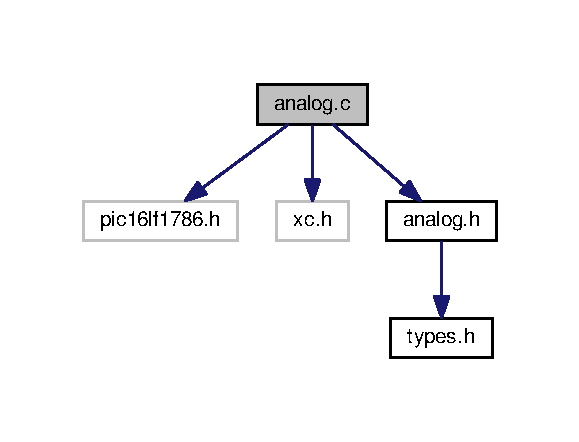
\includegraphics[width=278pt]{analog_8c__incl}
\end{center}
\end{figure}
\subsection*{Functions}
\begin{DoxyCompactItemize}
\item 
void \hyperlink{analog_8c_afc48ece98916606fadaade584b07b0f6}{analog\+\_\+start} (\hyperlink{analog_8h_a5498375a05ccaf5bb3ee237c052f4aba}{analog\+\_\+voltage\+\_\+reference\+\_\+positive\+\_\+t} voltage\+\_\+reference\+\_\+positive, \hyperlink{analog_8h_a785746a4a28aff14d6cf9165e6f4ac5a}{analog\+\_\+voltage\+\_\+reference\+\_\+negative\+\_\+t} voltage\+\_\+reference\+\_\+negative, \hyperlink{analog_8h_a5183d8e7b75549dc41e4866d5ed5c45b}{analog\+\_\+conversion\+\_\+clock\+\_\+t} conversion\+\_\+clock, \hyperlink{analog_8h_a209fd41add1725565eaff3b773da51dc}{analog\+\_\+result\+\_\+format\+\_\+t} analog\+\_\+result\+\_\+format, \hyperlink{analog_8h_a39823aa8eada1a84d236b5887f6b614c}{analog\+\_\+result\+\_\+mode\+\_\+bit\+\_\+t} analog\+\_\+result\+\_\+mode\+\_\+bit, \hyperlink{analog_8h_aaac550cf000789bda83df7d9e151e8a4}{analog\+\_\+channel\+\_\+select\+\_\+t} channel\+\_\+select)
\item 
void \hyperlink{analog_8c_a1c674cc7687a16cd39a0b79caa7d1709}{analog\+\_\+channel\+\_\+select} (\hyperlink{analog_8h_aaac550cf000789bda83df7d9e151e8a4}{analog\+\_\+channel\+\_\+select\+\_\+t} channel\+\_\+select, \hyperlink{stdint_8h_aba7bc1797add20fe3efdf37ced1182c5}{uint8\+\_\+t} skip\+\_\+delay)
\item 
\hyperlink{stdint_8h_a1f1825b69244eb3ad2c7165ddc99c956}{uint16\+\_\+t} \hyperlink{analog_8c_a2da12556578d87f18cf7fc8393e566b1}{analog\+\_\+read\+\_\+interrupt\+\_\+get\+\_\+value} ()
\item 
\hyperlink{stdint_8h_a1f1825b69244eb3ad2c7165ddc99c956}{uint16\+\_\+t} \hyperlink{analog_8c_a5200646868c21e68affdeb3364ad5845}{analog\+\_\+read\+\_\+lock} ()
\item 
void \hyperlink{analog_8c_aba0c8a3e463e8317f867bc7e5577122f}{analog\+\_\+read\+\_\+interrupt} (\hyperlink{types_8h_aa8204afb245708cfdad3878a09f1c83e}{callback\+\_\+isr\+\_\+t} analog\+\_\+callback\+\_\+done)
\item 
void \hyperlink{analog_8c_afb7f46c1782e82e14bd7f22a841142de}{analog\+\_\+read\+\_\+isr} ()
\end{DoxyCompactItemize}
\subsection*{Variables}
\begin{DoxyCompactItemize}
\item 
\hyperlink{types_8h_aa8204afb245708cfdad3878a09f1c83e}{callback\+\_\+isr\+\_\+t} \hyperlink{analog_8c_ac0b7450a742ce341dbe8e06e18b3be09}{\+\_\+analog\+\_\+callback\+\_\+isr}
\end{DoxyCompactItemize}


\subsection{Function Documentation}
\hypertarget{analog_8c_a1c674cc7687a16cd39a0b79caa7d1709}{\index{analog.\+c@{analog.\+c}!analog\+\_\+channel\+\_\+select@{analog\+\_\+channel\+\_\+select}}
\index{analog\+\_\+channel\+\_\+select@{analog\+\_\+channel\+\_\+select}!analog.\+c@{analog.\+c}}
\subsubsection[{analog\+\_\+channel\+\_\+select}]{\setlength{\rightskip}{0pt plus 5cm}void analog\+\_\+channel\+\_\+select (
\begin{DoxyParamCaption}
\item[{{\bf analog\+\_\+channel\+\_\+select\+\_\+t}}]{channel\+\_\+select, }
\item[{{\bf uint8\+\_\+t}}]{skip\+\_\+delay}
\end{DoxyParamCaption}
)}}\label{analog_8c_a1c674cc7687a16cd39a0b79caa7d1709}
Faz a sele��o do canal que ser� usado. 
\begin{DoxyParams}{Parameters}
{\em channel\+\_\+select} & O canal que ser� usado \\
\hline
{\em skip\+\_\+delay} & Quando verdadeiro, ignora o delay obrigat�rio, necess�rio para troca do canal. \\
\hline
\end{DoxyParams}
\hypertarget{analog_8c_aba0c8a3e463e8317f867bc7e5577122f}{\index{analog.\+c@{analog.\+c}!analog\+\_\+read\+\_\+interrupt@{analog\+\_\+read\+\_\+interrupt}}
\index{analog\+\_\+read\+\_\+interrupt@{analog\+\_\+read\+\_\+interrupt}!analog.\+c@{analog.\+c}}
\subsubsection[{analog\+\_\+read\+\_\+interrupt}]{\setlength{\rightskip}{0pt plus 5cm}void analog\+\_\+read\+\_\+interrupt (
\begin{DoxyParamCaption}
\item[{{\bf callback\+\_\+isr\+\_\+t}}]{analog\+\_\+callback\+\_\+done}
\end{DoxyParamCaption}
)}}\label{analog_8c_aba0c8a3e463e8317f867bc7e5577122f}
Faz a convers�o de anal�gico para digital, utilizando interrup��o. 
\begin{DoxyParams}{Parameters}
{\em analog\+\_\+callback\+\_\+done} & Rotina que ser� executada quando a interrup��o ocorrer. \\
\hline
\end{DoxyParams}
\begin{DoxyRemark}{Remarks}
Para recuperar o valor convertido, utilize a fun��o analog\+\_\+read\+\_\+interrupt\+\_\+get\+\_\+value 
\end{DoxyRemark}
\hypertarget{analog_8c_a2da12556578d87f18cf7fc8393e566b1}{\index{analog.\+c@{analog.\+c}!analog\+\_\+read\+\_\+interrupt\+\_\+get\+\_\+value@{analog\+\_\+read\+\_\+interrupt\+\_\+get\+\_\+value}}
\index{analog\+\_\+read\+\_\+interrupt\+\_\+get\+\_\+value@{analog\+\_\+read\+\_\+interrupt\+\_\+get\+\_\+value}!analog.\+c@{analog.\+c}}
\subsubsection[{analog\+\_\+read\+\_\+interrupt\+\_\+get\+\_\+value}]{\setlength{\rightskip}{0pt plus 5cm}{\bf uint16\+\_\+t} analog\+\_\+read\+\_\+interrupt\+\_\+get\+\_\+value (
\begin{DoxyParamCaption}
{}
\end{DoxyParamCaption}
)}}\label{analog_8c_a2da12556578d87f18cf7fc8393e566b1}
Recupera o valor da convers�o anal�gico-\/digital, j� convertido para uso normal. \begin{DoxyReturn}{Returns}
O valor convertido 
\end{DoxyReturn}
\hypertarget{analog_8c_afb7f46c1782e82e14bd7f22a841142de}{\index{analog.\+c@{analog.\+c}!analog\+\_\+read\+\_\+isr@{analog\+\_\+read\+\_\+isr}}
\index{analog\+\_\+read\+\_\+isr@{analog\+\_\+read\+\_\+isr}!analog.\+c@{analog.\+c}}
\subsubsection[{analog\+\_\+read\+\_\+isr}]{\setlength{\rightskip}{0pt plus 5cm}void analog\+\_\+read\+\_\+isr (
\begin{DoxyParamCaption}
{}
\end{DoxyParamCaption}
)}}\label{analog_8c_afb7f46c1782e82e14bd7f22a841142de}
Fun��o chamada na rotina de interrup��o. \begin{DoxyRemark}{Remarks}
Est� fun��o s� deve ser chamada na interrup��o. O programador final n�o precisa invocar ela. 
\end{DoxyRemark}
\hypertarget{analog_8c_a5200646868c21e68affdeb3364ad5845}{\index{analog.\+c@{analog.\+c}!analog\+\_\+read\+\_\+lock@{analog\+\_\+read\+\_\+lock}}
\index{analog\+\_\+read\+\_\+lock@{analog\+\_\+read\+\_\+lock}!analog.\+c@{analog.\+c}}
\subsubsection[{analog\+\_\+read\+\_\+lock}]{\setlength{\rightskip}{0pt plus 5cm}{\bf uint16\+\_\+t} analog\+\_\+read\+\_\+lock (
\begin{DoxyParamCaption}
{}
\end{DoxyParamCaption}
)}}\label{analog_8c_a5200646868c21e68affdeb3364ad5845}
Faz uma convers�o anal�gico digital em modo de espera. \begin{DoxyReturn}{Returns}
O valor convertido. 
\end{DoxyReturn}
\hypertarget{analog_8c_afc48ece98916606fadaade584b07b0f6}{\index{analog.\+c@{analog.\+c}!analog\+\_\+start@{analog\+\_\+start}}
\index{analog\+\_\+start@{analog\+\_\+start}!analog.\+c@{analog.\+c}}
\subsubsection[{analog\+\_\+start}]{\setlength{\rightskip}{0pt plus 5cm}void analog\+\_\+start (
\begin{DoxyParamCaption}
\item[{{\bf analog\+\_\+voltage\+\_\+reference\+\_\+positive\+\_\+t}}]{voltage\+\_\+reference\+\_\+positive, }
\item[{{\bf analog\+\_\+voltage\+\_\+reference\+\_\+negative\+\_\+t}}]{voltage\+\_\+reference\+\_\+negative, }
\item[{{\bf analog\+\_\+conversion\+\_\+clock\+\_\+t}}]{conversion\+\_\+clock, }
\item[{{\bf analog\+\_\+result\+\_\+format\+\_\+t}}]{analog\+\_\+result\+\_\+format, }
\item[{{\bf analog\+\_\+result\+\_\+mode\+\_\+bit\+\_\+t}}]{analog\+\_\+result\+\_\+mode\+\_\+bit, }
\item[{{\bf analog\+\_\+channel\+\_\+select\+\_\+t}}]{channel\+\_\+select}
\end{DoxyParamCaption}
)}}\label{analog_8c_afc48ece98916606fadaade584b07b0f6}
Inicializa e ativa o uso do conversor Anal�gico/\+Digital. 
\begin{DoxyParams}{Parameters}
{\em voltage\+\_\+reference\+\_\+positive} & \\
\hline
{\em voltage\+\_\+reference\+\_\+negative} & \\
\hline
{\em conversion\+\_\+clock} & \\
\hline
{\em analog\+\_\+result\+\_\+format} & \\
\hline
{\em analog\+\_\+result\+\_\+mode\+\_\+bit} & \\
\hline
{\em channel\+\_\+select} & \\
\hline
\end{DoxyParams}


\subsection{Variable Documentation}
\hypertarget{analog_8c_ac0b7450a742ce341dbe8e06e18b3be09}{\index{analog.\+c@{analog.\+c}!\+\_\+analog\+\_\+callback\+\_\+isr@{\+\_\+analog\+\_\+callback\+\_\+isr}}
\index{\+\_\+analog\+\_\+callback\+\_\+isr@{\+\_\+analog\+\_\+callback\+\_\+isr}!analog.\+c@{analog.\+c}}
\subsubsection[{\+\_\+analog\+\_\+callback\+\_\+isr}]{\setlength{\rightskip}{0pt plus 5cm}{\bf callback\+\_\+isr\+\_\+t} \+\_\+analog\+\_\+callback\+\_\+isr}}\label{analog_8c_ac0b7450a742ce341dbe8e06e18b3be09}

\hypertarget{analog_8h}{\section{analog.\+h File Reference}
\label{analog_8h}\index{analog.\+h@{analog.\+h}}
}
{\ttfamily \#include \char`\"{}types.\+h\char`\"{}}\\*
Include dependency graph for analog.\+h\+:\nopagebreak
\begin{figure}[H]
\begin{center}
\leavevmode
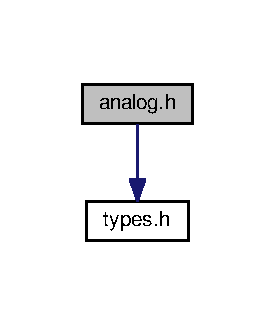
\includegraphics[width=132pt]{analog_8h__incl}
\end{center}
\end{figure}
This graph shows which files directly or indirectly include this file\+:\nopagebreak
\begin{figure}[H]
\begin{center}
\leavevmode
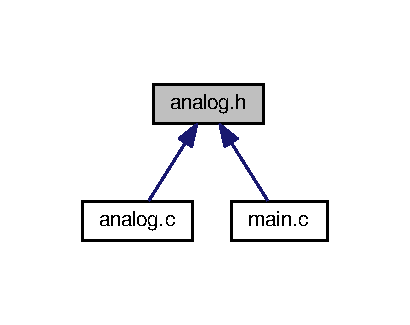
\includegraphics[width=197pt]{analog_8h__dep__incl}
\end{center}
\end{figure}
\subsection*{Typedefs}
\begin{DoxyCompactItemize}
\item 
typedef enum \\*
\hyperlink{analog_8h_a82f5c5e5c9b431aef9fe84b261575b01}{analog\+\_\+voltage\+\_\+reference\+\_\+positive\+\_\+e} \hyperlink{analog_8h_a5498375a05ccaf5bb3ee237c052f4aba}{analog\+\_\+voltage\+\_\+reference\+\_\+positive\+\_\+t}
\item 
typedef enum \\*
\hyperlink{analog_8h_a4f20aa9e4d38bd01c8d83730aae07bed}{analog\+\_\+voltage\+\_\+reference\+\_\+negative\+\_\+e} \hyperlink{analog_8h_a785746a4a28aff14d6cf9165e6f4ac5a}{analog\+\_\+voltage\+\_\+reference\+\_\+negative\+\_\+t}
\item 
typedef enum \\*
\hyperlink{analog_8h_af53693509ee61f2936ef96c1886433cc}{analog\+\_\+conversion\+\_\+clock\+\_\+e} \hyperlink{analog_8h_a5183d8e7b75549dc41e4866d5ed5c45b}{analog\+\_\+conversion\+\_\+clock\+\_\+t}
\item 
typedef enum \hyperlink{analog_8h_a27ef65da7bd4dd57fc27e658eaa7eee9}{analog\+\_\+result\+\_\+format\+\_\+e} \hyperlink{analog_8h_a209fd41add1725565eaff3b773da51dc}{analog\+\_\+result\+\_\+format\+\_\+t}
\item 
typedef enum \\*
\hyperlink{analog_8h_aa2d1377fd93fdbd5a5c95c0dc4757ecc}{analog\+\_\+result\+\_\+mode\+\_\+bit\+\_\+e} \hyperlink{analog_8h_a39823aa8eada1a84d236b5887f6b614c}{analog\+\_\+result\+\_\+mode\+\_\+bit\+\_\+t}
\item 
typedef enum \\*
\hyperlink{analog_8h_af2cbf1d809212e01f5b4895fc392317b}{analog\+\_\+channel\+\_\+select\+\_\+e} \hyperlink{analog_8h_aaac550cf000789bda83df7d9e151e8a4}{analog\+\_\+channel\+\_\+select\+\_\+t}
\end{DoxyCompactItemize}
\subsection*{Enumerations}
\begin{DoxyCompactItemize}
\item 
enum \hyperlink{analog_8h_a82f5c5e5c9b431aef9fe84b261575b01}{analog\+\_\+voltage\+\_\+reference\+\_\+positive\+\_\+e} \{ \hyperlink{analog_8h_a82f5c5e5c9b431aef9fe84b261575b01a8deaeb1c9286ca5b27028d32e440d5a5}{analog\+\_\+voltage\+\_\+reference\+\_\+positive\+\_\+vdd} = 0b00, 
\hyperlink{analog_8h_a82f5c5e5c9b431aef9fe84b261575b01a38ba8ac1bbe48a253c43362b5823a175}{analog\+\_\+voltage\+\_\+reference\+\_\+positive\+\_\+vrefp} = 0b01, 
\hyperlink{analog_8h_a82f5c5e5c9b431aef9fe84b261575b01af4a7efd299aa697287b31a2a029152d7}{analog\+\_\+voltage\+\_\+reference\+\_\+positive\+\_\+fvr} = 0b11
 \}
\item 
enum \hyperlink{analog_8h_a4f20aa9e4d38bd01c8d83730aae07bed}{analog\+\_\+voltage\+\_\+reference\+\_\+negative\+\_\+e} \{ \hyperlink{analog_8h_a4f20aa9e4d38bd01c8d83730aae07beda8ae230b3c54f93adc50b1f51fe80bb11}{analog\+\_\+voltage\+\_\+reference\+\_\+negative\+\_\+vss} = 0b0, 
\hyperlink{analog_8h_a4f20aa9e4d38bd01c8d83730aae07beda5a61538c0a1a3c1c984b805f16bcf5aa}{analog\+\_\+voltage\+\_\+reference\+\_\+negative\+\_\+vrefm} = 0b1
 \}
\item 
enum \hyperlink{analog_8h_af53693509ee61f2936ef96c1886433cc}{analog\+\_\+conversion\+\_\+clock\+\_\+e} \{ \\*
\hyperlink{analog_8h_af53693509ee61f2936ef96c1886433cca5b517e1588538ab7d5f7749bd08c96b3}{analog\+\_\+conversion\+\_\+clock\+\_\+fosc\+\_\+2} = 0b000, 
\hyperlink{analog_8h_af53693509ee61f2936ef96c1886433cca0cc4a9505db207616af34a34bffcabc7}{analog\+\_\+conversion\+\_\+clock\+\_\+fosc\+\_\+4} = 0b100, 
\hyperlink{analog_8h_af53693509ee61f2936ef96c1886433cca9866aa8fc38f9b24add66f8ea3985cef}{analog\+\_\+conversion\+\_\+clock\+\_\+fosc\+\_\+8} = 0b001, 
\hyperlink{analog_8h_af53693509ee61f2936ef96c1886433cca53cd5b22ce66693d0b9ad41ca9af2365}{analog\+\_\+conversion\+\_\+clock\+\_\+fosc\+\_\+16} = 0b101, 
\\*
\hyperlink{analog_8h_af53693509ee61f2936ef96c1886433cca881f10505829403e15b5bce071de7751}{analog\+\_\+conversion\+\_\+clock\+\_\+fosc\+\_\+32} = 0b010, 
\hyperlink{analog_8h_af53693509ee61f2936ef96c1886433ccab0e9867790d5c15fdeb4f8da3113dada}{analog\+\_\+conversion\+\_\+clock\+\_\+fosc\+\_\+64} = 0b110, 
\hyperlink{analog_8h_af53693509ee61f2936ef96c1886433ccaef70fdf9624751d4c022c427a6fdc7ba}{analog\+\_\+conversion\+\_\+clock\+\_\+frc} = 0b011
 \}
\item 
enum \hyperlink{analog_8h_a27ef65da7bd4dd57fc27e658eaa7eee9}{analog\+\_\+result\+\_\+format\+\_\+e} \{ \hyperlink{analog_8h_a27ef65da7bd4dd57fc27e658eaa7eee9a567afeaeec14ea2047619e2f007abd83}{analog\+\_\+result\+\_\+format\+\_\+sign\+\_\+magnitude} = 0b0, 
\hyperlink{analog_8h_a27ef65da7bd4dd57fc27e658eaa7eee9a22848fb1ed118d56dde2af1c8fa00895}{analog\+\_\+result\+\_\+format\+\_\+twos\+\_\+compliment} = 0b1
 \}
\item 
enum \hyperlink{analog_8h_aa2d1377fd93fdbd5a5c95c0dc4757ecc}{analog\+\_\+result\+\_\+mode\+\_\+bit\+\_\+e} \{ \hyperlink{analog_8h_aa2d1377fd93fdbd5a5c95c0dc4757ecca337e682c14b5ee5b0fc6ef02a0481863}{analog\+\_\+result\+\_\+mode\+\_\+bit\+\_\+12} = 0b0, 
\hyperlink{analog_8h_aa2d1377fd93fdbd5a5c95c0dc4757eccaedf4139d4c2c26db33191bc054b7342b}{analog\+\_\+result\+\_\+mode\+\_\+bit\+\_\+10} = 0b1
 \}
\item 
enum \hyperlink{analog_8h_af2cbf1d809212e01f5b4895fc392317b}{analog\+\_\+channel\+\_\+select\+\_\+e} \{ \hyperlink{analog_8h_af2cbf1d809212e01f5b4895fc392317ba7fca399d134ce3d8e42dbe7aa6322ebf}{analog\+\_\+channel\+\_\+select\+\_\+0} = 0b00000
 \}
\end{DoxyCompactItemize}
\subsection*{Functions}
\begin{DoxyCompactItemize}
\item 
void \hyperlink{analog_8h_afc48ece98916606fadaade584b07b0f6}{analog\+\_\+start} (\hyperlink{analog_8h_a5498375a05ccaf5bb3ee237c052f4aba}{analog\+\_\+voltage\+\_\+reference\+\_\+positive\+\_\+t} voltage\+\_\+reference\+\_\+positive, \hyperlink{analog_8h_a785746a4a28aff14d6cf9165e6f4ac5a}{analog\+\_\+voltage\+\_\+reference\+\_\+negative\+\_\+t} voltage\+\_\+reference\+\_\+negative, \hyperlink{analog_8h_a5183d8e7b75549dc41e4866d5ed5c45b}{analog\+\_\+conversion\+\_\+clock\+\_\+t} conversion\+\_\+clock, \hyperlink{analog_8h_a209fd41add1725565eaff3b773da51dc}{analog\+\_\+result\+\_\+format\+\_\+t} analog\+\_\+result\+\_\+format, \hyperlink{analog_8h_a39823aa8eada1a84d236b5887f6b614c}{analog\+\_\+result\+\_\+mode\+\_\+bit\+\_\+t} analog\+\_\+result\+\_\+mode\+\_\+bit, \hyperlink{analog_8h_aaac550cf000789bda83df7d9e151e8a4}{analog\+\_\+channel\+\_\+select\+\_\+t} channel\+\_\+select)
\item 
void \hyperlink{analog_8h_a1c674cc7687a16cd39a0b79caa7d1709}{analog\+\_\+channel\+\_\+select} (\hyperlink{analog_8h_aaac550cf000789bda83df7d9e151e8a4}{analog\+\_\+channel\+\_\+select\+\_\+t} channel\+\_\+select, \hyperlink{stdint_8h_aba7bc1797add20fe3efdf37ced1182c5}{uint8\+\_\+t} skip\+\_\+delay)
\item 
\hyperlink{stdint_8h_a1f1825b69244eb3ad2c7165ddc99c956}{uint16\+\_\+t} \hyperlink{analog_8h_a5200646868c21e68affdeb3364ad5845}{analog\+\_\+read\+\_\+lock} ()
\item 
void \hyperlink{analog_8h_aba0c8a3e463e8317f867bc7e5577122f}{analog\+\_\+read\+\_\+interrupt} (\hyperlink{types_8h_aa8204afb245708cfdad3878a09f1c83e}{callback\+\_\+isr\+\_\+t} analog\+\_\+callback\+\_\+done)
\item 
\hyperlink{stdint_8h_a1f1825b69244eb3ad2c7165ddc99c956}{uint16\+\_\+t} \hyperlink{analog_8h_a2da12556578d87f18cf7fc8393e566b1}{analog\+\_\+read\+\_\+interrupt\+\_\+get\+\_\+value} ()
\item 
void \hyperlink{analog_8h_afb7f46c1782e82e14bd7f22a841142de}{analog\+\_\+read\+\_\+isr} ()
\end{DoxyCompactItemize}


\subsection{Typedef Documentation}
\hypertarget{analog_8h_aaac550cf000789bda83df7d9e151e8a4}{\index{analog.\+h@{analog.\+h}!analog\+\_\+channel\+\_\+select\+\_\+t@{analog\+\_\+channel\+\_\+select\+\_\+t}}
\index{analog\+\_\+channel\+\_\+select\+\_\+t@{analog\+\_\+channel\+\_\+select\+\_\+t}!analog.\+h@{analog.\+h}}
\subsubsection[{analog\+\_\+channel\+\_\+select\+\_\+t}]{\setlength{\rightskip}{0pt plus 5cm}typedef enum {\bf analog\+\_\+channel\+\_\+select\+\_\+e}  {\bf analog\+\_\+channel\+\_\+select\+\_\+t}}}\label{analog_8h_aaac550cf000789bda83df7d9e151e8a4}
Indica qual canal dever� ser selecionado. \begin{DoxyRefDesc}{Todo}
\item[\hyperlink{todo__todo000001}{Todo}]Por hora, apenas o canal 0 foi implementado. Ver a necessidade de utilizar os outros. \end{DoxyRefDesc}
\hypertarget{analog_8h_a5183d8e7b75549dc41e4866d5ed5c45b}{\index{analog.\+h@{analog.\+h}!analog\+\_\+conversion\+\_\+clock\+\_\+t@{analog\+\_\+conversion\+\_\+clock\+\_\+t}}
\index{analog\+\_\+conversion\+\_\+clock\+\_\+t@{analog\+\_\+conversion\+\_\+clock\+\_\+t}!analog.\+h@{analog.\+h}}
\subsubsection[{analog\+\_\+conversion\+\_\+clock\+\_\+t}]{\setlength{\rightskip}{0pt plus 5cm}typedef enum {\bf analog\+\_\+conversion\+\_\+clock\+\_\+e}  {\bf analog\+\_\+conversion\+\_\+clock\+\_\+t}}}\label{analog_8h_a5183d8e7b75549dc41e4866d5ed5c45b}
\hypertarget{analog_8h_a209fd41add1725565eaff3b773da51dc}{\index{analog.\+h@{analog.\+h}!analog\+\_\+result\+\_\+format\+\_\+t@{analog\+\_\+result\+\_\+format\+\_\+t}}
\index{analog\+\_\+result\+\_\+format\+\_\+t@{analog\+\_\+result\+\_\+format\+\_\+t}!analog.\+h@{analog.\+h}}
\subsubsection[{analog\+\_\+result\+\_\+format\+\_\+t}]{\setlength{\rightskip}{0pt plus 5cm}typedef enum {\bf analog\+\_\+result\+\_\+format\+\_\+e}  {\bf analog\+\_\+result\+\_\+format\+\_\+t}}}\label{analog_8h_a209fd41add1725565eaff3b773da51dc}
Indica o formato do resultado da convers�o. \hypertarget{analog_8h_a39823aa8eada1a84d236b5887f6b614c}{\index{analog.\+h@{analog.\+h}!analog\+\_\+result\+\_\+mode\+\_\+bit\+\_\+t@{analog\+\_\+result\+\_\+mode\+\_\+bit\+\_\+t}}
\index{analog\+\_\+result\+\_\+mode\+\_\+bit\+\_\+t@{analog\+\_\+result\+\_\+mode\+\_\+bit\+\_\+t}!analog.\+h@{analog.\+h}}
\subsubsection[{analog\+\_\+result\+\_\+mode\+\_\+bit\+\_\+t}]{\setlength{\rightskip}{0pt plus 5cm}typedef enum {\bf analog\+\_\+result\+\_\+mode\+\_\+bit\+\_\+e}  {\bf analog\+\_\+result\+\_\+mode\+\_\+bit\+\_\+t}}}\label{analog_8h_a39823aa8eada1a84d236b5887f6b614c}
Indica quantos bits ser�o utilizados na convers�o do sinal. \hypertarget{analog_8h_a785746a4a28aff14d6cf9165e6f4ac5a}{\index{analog.\+h@{analog.\+h}!analog\+\_\+voltage\+\_\+reference\+\_\+negative\+\_\+t@{analog\+\_\+voltage\+\_\+reference\+\_\+negative\+\_\+t}}
\index{analog\+\_\+voltage\+\_\+reference\+\_\+negative\+\_\+t@{analog\+\_\+voltage\+\_\+reference\+\_\+negative\+\_\+t}!analog.\+h@{analog.\+h}}
\subsubsection[{analog\+\_\+voltage\+\_\+reference\+\_\+negative\+\_\+t}]{\setlength{\rightskip}{0pt plus 5cm}typedef enum {\bf analog\+\_\+voltage\+\_\+reference\+\_\+negative\+\_\+e}  {\bf analog\+\_\+voltage\+\_\+reference\+\_\+negative\+\_\+t}}}\label{analog_8h_a785746a4a28aff14d6cf9165e6f4ac5a}
\hypertarget{analog_8h_a5498375a05ccaf5bb3ee237c052f4aba}{\index{analog.\+h@{analog.\+h}!analog\+\_\+voltage\+\_\+reference\+\_\+positive\+\_\+t@{analog\+\_\+voltage\+\_\+reference\+\_\+positive\+\_\+t}}
\index{analog\+\_\+voltage\+\_\+reference\+\_\+positive\+\_\+t@{analog\+\_\+voltage\+\_\+reference\+\_\+positive\+\_\+t}!analog.\+h@{analog.\+h}}
\subsubsection[{analog\+\_\+voltage\+\_\+reference\+\_\+positive\+\_\+t}]{\setlength{\rightskip}{0pt plus 5cm}typedef enum {\bf analog\+\_\+voltage\+\_\+reference\+\_\+positive\+\_\+e}  {\bf analog\+\_\+voltage\+\_\+reference\+\_\+positive\+\_\+t}}}\label{analog_8h_a5498375a05ccaf5bb3ee237c052f4aba}


\subsection{Enumeration Type Documentation}
\hypertarget{analog_8h_af2cbf1d809212e01f5b4895fc392317b}{\index{analog.\+h@{analog.\+h}!analog\+\_\+channel\+\_\+select\+\_\+e@{analog\+\_\+channel\+\_\+select\+\_\+e}}
\index{analog\+\_\+channel\+\_\+select\+\_\+e@{analog\+\_\+channel\+\_\+select\+\_\+e}!analog.\+h@{analog.\+h}}
\subsubsection[{analog\+\_\+channel\+\_\+select\+\_\+e}]{\setlength{\rightskip}{0pt plus 5cm}enum {\bf analog\+\_\+channel\+\_\+select\+\_\+e}}}\label{analog_8h_af2cbf1d809212e01f5b4895fc392317b}
Indica qual canal dever� ser selecionado. \begin{DoxyRefDesc}{Todo}
\item[\hyperlink{todo__todo000001}{Todo}]Por hora, apenas o canal 0 foi implementado. Ver a necessidade de utilizar os outros. \end{DoxyRefDesc}
\begin{Desc}
\item[Enumerator]\par
\begin{description}
\index{analog\+\_\+channel\+\_\+select\+\_\+0@{analog\+\_\+channel\+\_\+select\+\_\+0}!analog.\+h@{analog.\+h}}\index{analog.\+h@{analog.\+h}!analog\+\_\+channel\+\_\+select\+\_\+0@{analog\+\_\+channel\+\_\+select\+\_\+0}}\item[{\em 
\hypertarget{analog_8h_af2cbf1d809212e01f5b4895fc392317ba7fca399d134ce3d8e42dbe7aa6322ebf}{analog\+\_\+channel\+\_\+select\+\_\+0}\label{analog_8h_af2cbf1d809212e01f5b4895fc392317ba7fca399d134ce3d8e42dbe7aa6322ebf}
}]\end{description}
\end{Desc}
\hypertarget{analog_8h_af53693509ee61f2936ef96c1886433cc}{\index{analog.\+h@{analog.\+h}!analog\+\_\+conversion\+\_\+clock\+\_\+e@{analog\+\_\+conversion\+\_\+clock\+\_\+e}}
\index{analog\+\_\+conversion\+\_\+clock\+\_\+e@{analog\+\_\+conversion\+\_\+clock\+\_\+e}!analog.\+h@{analog.\+h}}
\subsubsection[{analog\+\_\+conversion\+\_\+clock\+\_\+e}]{\setlength{\rightskip}{0pt plus 5cm}enum {\bf analog\+\_\+conversion\+\_\+clock\+\_\+e}}}\label{analog_8h_af53693509ee61f2936ef96c1886433cc}
\begin{Desc}
\item[Enumerator]\par
\begin{description}
\index{analog\+\_\+conversion\+\_\+clock\+\_\+fosc\+\_\+2@{analog\+\_\+conversion\+\_\+clock\+\_\+fosc\+\_\+2}!analog.\+h@{analog.\+h}}\index{analog.\+h@{analog.\+h}!analog\+\_\+conversion\+\_\+clock\+\_\+fosc\+\_\+2@{analog\+\_\+conversion\+\_\+clock\+\_\+fosc\+\_\+2}}\item[{\em 
\hypertarget{analog_8h_af53693509ee61f2936ef96c1886433cca5b517e1588538ab7d5f7749bd08c96b3}{analog\+\_\+conversion\+\_\+clock\+\_\+fosc\+\_\+2}\label{analog_8h_af53693509ee61f2936ef96c1886433cca5b517e1588538ab7d5f7749bd08c96b3}
}]\index{analog\+\_\+conversion\+\_\+clock\+\_\+fosc\+\_\+4@{analog\+\_\+conversion\+\_\+clock\+\_\+fosc\+\_\+4}!analog.\+h@{analog.\+h}}\index{analog.\+h@{analog.\+h}!analog\+\_\+conversion\+\_\+clock\+\_\+fosc\+\_\+4@{analog\+\_\+conversion\+\_\+clock\+\_\+fosc\+\_\+4}}\item[{\em 
\hypertarget{analog_8h_af53693509ee61f2936ef96c1886433cca0cc4a9505db207616af34a34bffcabc7}{analog\+\_\+conversion\+\_\+clock\+\_\+fosc\+\_\+4}\label{analog_8h_af53693509ee61f2936ef96c1886433cca0cc4a9505db207616af34a34bffcabc7}
}]\index{analog\+\_\+conversion\+\_\+clock\+\_\+fosc\+\_\+8@{analog\+\_\+conversion\+\_\+clock\+\_\+fosc\+\_\+8}!analog.\+h@{analog.\+h}}\index{analog.\+h@{analog.\+h}!analog\+\_\+conversion\+\_\+clock\+\_\+fosc\+\_\+8@{analog\+\_\+conversion\+\_\+clock\+\_\+fosc\+\_\+8}}\item[{\em 
\hypertarget{analog_8h_af53693509ee61f2936ef96c1886433cca9866aa8fc38f9b24add66f8ea3985cef}{analog\+\_\+conversion\+\_\+clock\+\_\+fosc\+\_\+8}\label{analog_8h_af53693509ee61f2936ef96c1886433cca9866aa8fc38f9b24add66f8ea3985cef}
}]\index{analog\+\_\+conversion\+\_\+clock\+\_\+fosc\+\_\+16@{analog\+\_\+conversion\+\_\+clock\+\_\+fosc\+\_\+16}!analog.\+h@{analog.\+h}}\index{analog.\+h@{analog.\+h}!analog\+\_\+conversion\+\_\+clock\+\_\+fosc\+\_\+16@{analog\+\_\+conversion\+\_\+clock\+\_\+fosc\+\_\+16}}\item[{\em 
\hypertarget{analog_8h_af53693509ee61f2936ef96c1886433cca53cd5b22ce66693d0b9ad41ca9af2365}{analog\+\_\+conversion\+\_\+clock\+\_\+fosc\+\_\+16}\label{analog_8h_af53693509ee61f2936ef96c1886433cca53cd5b22ce66693d0b9ad41ca9af2365}
}]\index{analog\+\_\+conversion\+\_\+clock\+\_\+fosc\+\_\+32@{analog\+\_\+conversion\+\_\+clock\+\_\+fosc\+\_\+32}!analog.\+h@{analog.\+h}}\index{analog.\+h@{analog.\+h}!analog\+\_\+conversion\+\_\+clock\+\_\+fosc\+\_\+32@{analog\+\_\+conversion\+\_\+clock\+\_\+fosc\+\_\+32}}\item[{\em 
\hypertarget{analog_8h_af53693509ee61f2936ef96c1886433cca881f10505829403e15b5bce071de7751}{analog\+\_\+conversion\+\_\+clock\+\_\+fosc\+\_\+32}\label{analog_8h_af53693509ee61f2936ef96c1886433cca881f10505829403e15b5bce071de7751}
}]\index{analog\+\_\+conversion\+\_\+clock\+\_\+fosc\+\_\+64@{analog\+\_\+conversion\+\_\+clock\+\_\+fosc\+\_\+64}!analog.\+h@{analog.\+h}}\index{analog.\+h@{analog.\+h}!analog\+\_\+conversion\+\_\+clock\+\_\+fosc\+\_\+64@{analog\+\_\+conversion\+\_\+clock\+\_\+fosc\+\_\+64}}\item[{\em 
\hypertarget{analog_8h_af53693509ee61f2936ef96c1886433ccab0e9867790d5c15fdeb4f8da3113dada}{analog\+\_\+conversion\+\_\+clock\+\_\+fosc\+\_\+64}\label{analog_8h_af53693509ee61f2936ef96c1886433ccab0e9867790d5c15fdeb4f8da3113dada}
}]\index{analog\+\_\+conversion\+\_\+clock\+\_\+frc@{analog\+\_\+conversion\+\_\+clock\+\_\+frc}!analog.\+h@{analog.\+h}}\index{analog.\+h@{analog.\+h}!analog\+\_\+conversion\+\_\+clock\+\_\+frc@{analog\+\_\+conversion\+\_\+clock\+\_\+frc}}\item[{\em 
\hypertarget{analog_8h_af53693509ee61f2936ef96c1886433ccaef70fdf9624751d4c022c427a6fdc7ba}{analog\+\_\+conversion\+\_\+clock\+\_\+frc}\label{analog_8h_af53693509ee61f2936ef96c1886433ccaef70fdf9624751d4c022c427a6fdc7ba}
}]\end{description}
\end{Desc}
\hypertarget{analog_8h_a27ef65da7bd4dd57fc27e658eaa7eee9}{\index{analog.\+h@{analog.\+h}!analog\+\_\+result\+\_\+format\+\_\+e@{analog\+\_\+result\+\_\+format\+\_\+e}}
\index{analog\+\_\+result\+\_\+format\+\_\+e@{analog\+\_\+result\+\_\+format\+\_\+e}!analog.\+h@{analog.\+h}}
\subsubsection[{analog\+\_\+result\+\_\+format\+\_\+e}]{\setlength{\rightskip}{0pt plus 5cm}enum {\bf analog\+\_\+result\+\_\+format\+\_\+e}}}\label{analog_8h_a27ef65da7bd4dd57fc27e658eaa7eee9}
Indica o formato do resultado da convers�o. \begin{Desc}
\item[Enumerator]\par
\begin{description}
\index{analog\+\_\+result\+\_\+format\+\_\+sign\+\_\+magnitude@{analog\+\_\+result\+\_\+format\+\_\+sign\+\_\+magnitude}!analog.\+h@{analog.\+h}}\index{analog.\+h@{analog.\+h}!analog\+\_\+result\+\_\+format\+\_\+sign\+\_\+magnitude@{analog\+\_\+result\+\_\+format\+\_\+sign\+\_\+magnitude}}\item[{\em 
\hypertarget{analog_8h_a27ef65da7bd4dd57fc27e658eaa7eee9a567afeaeec14ea2047619e2f007abd83}{analog\+\_\+result\+\_\+format\+\_\+sign\+\_\+magnitude}\label{analog_8h_a27ef65da7bd4dd57fc27e658eaa7eee9a567afeaeec14ea2047619e2f007abd83}
}]Sinal + Magnitude \index{analog\+\_\+result\+\_\+format\+\_\+twos\+\_\+compliment@{analog\+\_\+result\+\_\+format\+\_\+twos\+\_\+compliment}!analog.\+h@{analog.\+h}}\index{analog.\+h@{analog.\+h}!analog\+\_\+result\+\_\+format\+\_\+twos\+\_\+compliment@{analog\+\_\+result\+\_\+format\+\_\+twos\+\_\+compliment}}\item[{\em 
\hypertarget{analog_8h_a27ef65da7bd4dd57fc27e658eaa7eee9a22848fb1ed118d56dde2af1c8fa00895}{analog\+\_\+result\+\_\+format\+\_\+twos\+\_\+compliment}\label{analog_8h_a27ef65da7bd4dd57fc27e658eaa7eee9a22848fb1ed118d56dde2af1c8fa00895}
}]Complemento de 2 \end{description}
\end{Desc}
\hypertarget{analog_8h_aa2d1377fd93fdbd5a5c95c0dc4757ecc}{\index{analog.\+h@{analog.\+h}!analog\+\_\+result\+\_\+mode\+\_\+bit\+\_\+e@{analog\+\_\+result\+\_\+mode\+\_\+bit\+\_\+e}}
\index{analog\+\_\+result\+\_\+mode\+\_\+bit\+\_\+e@{analog\+\_\+result\+\_\+mode\+\_\+bit\+\_\+e}!analog.\+h@{analog.\+h}}
\subsubsection[{analog\+\_\+result\+\_\+mode\+\_\+bit\+\_\+e}]{\setlength{\rightskip}{0pt plus 5cm}enum {\bf analog\+\_\+result\+\_\+mode\+\_\+bit\+\_\+e}}}\label{analog_8h_aa2d1377fd93fdbd5a5c95c0dc4757ecc}
Indica quantos bits ser�o utilizados na convers�o do sinal. \begin{Desc}
\item[Enumerator]\par
\begin{description}
\index{analog\+\_\+result\+\_\+mode\+\_\+bit\+\_\+12@{analog\+\_\+result\+\_\+mode\+\_\+bit\+\_\+12}!analog.\+h@{analog.\+h}}\index{analog.\+h@{analog.\+h}!analog\+\_\+result\+\_\+mode\+\_\+bit\+\_\+12@{analog\+\_\+result\+\_\+mode\+\_\+bit\+\_\+12}}\item[{\em 
\hypertarget{analog_8h_aa2d1377fd93fdbd5a5c95c0dc4757ecca337e682c14b5ee5b0fc6ef02a0481863}{analog\+\_\+result\+\_\+mode\+\_\+bit\+\_\+12}\label{analog_8h_aa2d1377fd93fdbd5a5c95c0dc4757ecca337e682c14b5ee5b0fc6ef02a0481863}
}]Converte o sinal com 12 bits \index{analog\+\_\+result\+\_\+mode\+\_\+bit\+\_\+10@{analog\+\_\+result\+\_\+mode\+\_\+bit\+\_\+10}!analog.\+h@{analog.\+h}}\index{analog.\+h@{analog.\+h}!analog\+\_\+result\+\_\+mode\+\_\+bit\+\_\+10@{analog\+\_\+result\+\_\+mode\+\_\+bit\+\_\+10}}\item[{\em 
\hypertarget{analog_8h_aa2d1377fd93fdbd5a5c95c0dc4757eccaedf4139d4c2c26db33191bc054b7342b}{analog\+\_\+result\+\_\+mode\+\_\+bit\+\_\+10}\label{analog_8h_aa2d1377fd93fdbd5a5c95c0dc4757eccaedf4139d4c2c26db33191bc054b7342b}
}]Converte o sinal com 10 bits \end{description}
\end{Desc}
\hypertarget{analog_8h_a4f20aa9e4d38bd01c8d83730aae07bed}{\index{analog.\+h@{analog.\+h}!analog\+\_\+voltage\+\_\+reference\+\_\+negative\+\_\+e@{analog\+\_\+voltage\+\_\+reference\+\_\+negative\+\_\+e}}
\index{analog\+\_\+voltage\+\_\+reference\+\_\+negative\+\_\+e@{analog\+\_\+voltage\+\_\+reference\+\_\+negative\+\_\+e}!analog.\+h@{analog.\+h}}
\subsubsection[{analog\+\_\+voltage\+\_\+reference\+\_\+negative\+\_\+e}]{\setlength{\rightskip}{0pt plus 5cm}enum {\bf analog\+\_\+voltage\+\_\+reference\+\_\+negative\+\_\+e}}}\label{analog_8h_a4f20aa9e4d38bd01c8d83730aae07bed}
\begin{Desc}
\item[Enumerator]\par
\begin{description}
\index{analog\+\_\+voltage\+\_\+reference\+\_\+negative\+\_\+vss@{analog\+\_\+voltage\+\_\+reference\+\_\+negative\+\_\+vss}!analog.\+h@{analog.\+h}}\index{analog.\+h@{analog.\+h}!analog\+\_\+voltage\+\_\+reference\+\_\+negative\+\_\+vss@{analog\+\_\+voltage\+\_\+reference\+\_\+negative\+\_\+vss}}\item[{\em 
\hypertarget{analog_8h_a4f20aa9e4d38bd01c8d83730aae07beda8ae230b3c54f93adc50b1f51fe80bb11}{analog\+\_\+voltage\+\_\+reference\+\_\+negative\+\_\+vss}\label{analog_8h_a4f20aa9e4d38bd01c8d83730aae07beda8ae230b3c54f93adc50b1f51fe80bb11}
}]\index{analog\+\_\+voltage\+\_\+reference\+\_\+negative\+\_\+vrefm@{analog\+\_\+voltage\+\_\+reference\+\_\+negative\+\_\+vrefm}!analog.\+h@{analog.\+h}}\index{analog.\+h@{analog.\+h}!analog\+\_\+voltage\+\_\+reference\+\_\+negative\+\_\+vrefm@{analog\+\_\+voltage\+\_\+reference\+\_\+negative\+\_\+vrefm}}\item[{\em 
\hypertarget{analog_8h_a4f20aa9e4d38bd01c8d83730aae07beda5a61538c0a1a3c1c984b805f16bcf5aa}{analog\+\_\+voltage\+\_\+reference\+\_\+negative\+\_\+vrefm}\label{analog_8h_a4f20aa9e4d38bd01c8d83730aae07beda5a61538c0a1a3c1c984b805f16bcf5aa}
}]\end{description}
\end{Desc}
\hypertarget{analog_8h_a82f5c5e5c9b431aef9fe84b261575b01}{\index{analog.\+h@{analog.\+h}!analog\+\_\+voltage\+\_\+reference\+\_\+positive\+\_\+e@{analog\+\_\+voltage\+\_\+reference\+\_\+positive\+\_\+e}}
\index{analog\+\_\+voltage\+\_\+reference\+\_\+positive\+\_\+e@{analog\+\_\+voltage\+\_\+reference\+\_\+positive\+\_\+e}!analog.\+h@{analog.\+h}}
\subsubsection[{analog\+\_\+voltage\+\_\+reference\+\_\+positive\+\_\+e}]{\setlength{\rightskip}{0pt plus 5cm}enum {\bf analog\+\_\+voltage\+\_\+reference\+\_\+positive\+\_\+e}}}\label{analog_8h_a82f5c5e5c9b431aef9fe84b261575b01}
\begin{Desc}
\item[Enumerator]\par
\begin{description}
\index{analog\+\_\+voltage\+\_\+reference\+\_\+positive\+\_\+vdd@{analog\+\_\+voltage\+\_\+reference\+\_\+positive\+\_\+vdd}!analog.\+h@{analog.\+h}}\index{analog.\+h@{analog.\+h}!analog\+\_\+voltage\+\_\+reference\+\_\+positive\+\_\+vdd@{analog\+\_\+voltage\+\_\+reference\+\_\+positive\+\_\+vdd}}\item[{\em 
\hypertarget{analog_8h_a82f5c5e5c9b431aef9fe84b261575b01a8deaeb1c9286ca5b27028d32e440d5a5}{analog\+\_\+voltage\+\_\+reference\+\_\+positive\+\_\+vdd}\label{analog_8h_a82f5c5e5c9b431aef9fe84b261575b01a8deaeb1c9286ca5b27028d32e440d5a5}
}]\index{analog\+\_\+voltage\+\_\+reference\+\_\+positive\+\_\+vrefp@{analog\+\_\+voltage\+\_\+reference\+\_\+positive\+\_\+vrefp}!analog.\+h@{analog.\+h}}\index{analog.\+h@{analog.\+h}!analog\+\_\+voltage\+\_\+reference\+\_\+positive\+\_\+vrefp@{analog\+\_\+voltage\+\_\+reference\+\_\+positive\+\_\+vrefp}}\item[{\em 
\hypertarget{analog_8h_a82f5c5e5c9b431aef9fe84b261575b01a38ba8ac1bbe48a253c43362b5823a175}{analog\+\_\+voltage\+\_\+reference\+\_\+positive\+\_\+vrefp}\label{analog_8h_a82f5c5e5c9b431aef9fe84b261575b01a38ba8ac1bbe48a253c43362b5823a175}
}]\index{analog\+\_\+voltage\+\_\+reference\+\_\+positive\+\_\+fvr@{analog\+\_\+voltage\+\_\+reference\+\_\+positive\+\_\+fvr}!analog.\+h@{analog.\+h}}\index{analog.\+h@{analog.\+h}!analog\+\_\+voltage\+\_\+reference\+\_\+positive\+\_\+fvr@{analog\+\_\+voltage\+\_\+reference\+\_\+positive\+\_\+fvr}}\item[{\em 
\hypertarget{analog_8h_a82f5c5e5c9b431aef9fe84b261575b01af4a7efd299aa697287b31a2a029152d7}{analog\+\_\+voltage\+\_\+reference\+\_\+positive\+\_\+fvr}\label{analog_8h_a82f5c5e5c9b431aef9fe84b261575b01af4a7efd299aa697287b31a2a029152d7}
}]\end{description}
\end{Desc}


\subsection{Function Documentation}
\hypertarget{analog_8h_a1c674cc7687a16cd39a0b79caa7d1709}{\index{analog.\+h@{analog.\+h}!analog\+\_\+channel\+\_\+select@{analog\+\_\+channel\+\_\+select}}
\index{analog\+\_\+channel\+\_\+select@{analog\+\_\+channel\+\_\+select}!analog.\+h@{analog.\+h}}
\subsubsection[{analog\+\_\+channel\+\_\+select}]{\setlength{\rightskip}{0pt plus 5cm}void analog\+\_\+channel\+\_\+select (
\begin{DoxyParamCaption}
\item[{{\bf analog\+\_\+channel\+\_\+select\+\_\+t}}]{channel\+\_\+select, }
\item[{{\bf uint8\+\_\+t}}]{skip\+\_\+delay}
\end{DoxyParamCaption}
)}}\label{analog_8h_a1c674cc7687a16cd39a0b79caa7d1709}
Faz a sele��o do canal que ser� usado. 
\begin{DoxyParams}{Parameters}
{\em channel\+\_\+select} & O canal que ser� usado \\
\hline
{\em skip\+\_\+delay} & Quando verdadeiro, ignora o delay obrigat�rio, necess�rio para troca do canal. \\
\hline
\end{DoxyParams}
\hypertarget{analog_8h_aba0c8a3e463e8317f867bc7e5577122f}{\index{analog.\+h@{analog.\+h}!analog\+\_\+read\+\_\+interrupt@{analog\+\_\+read\+\_\+interrupt}}
\index{analog\+\_\+read\+\_\+interrupt@{analog\+\_\+read\+\_\+interrupt}!analog.\+h@{analog.\+h}}
\subsubsection[{analog\+\_\+read\+\_\+interrupt}]{\setlength{\rightskip}{0pt plus 5cm}void analog\+\_\+read\+\_\+interrupt (
\begin{DoxyParamCaption}
\item[{{\bf callback\+\_\+isr\+\_\+t}}]{analog\+\_\+callback\+\_\+done}
\end{DoxyParamCaption}
)}}\label{analog_8h_aba0c8a3e463e8317f867bc7e5577122f}
Faz a convers�o de anal�gico para digital, utilizando interrup��o. 
\begin{DoxyParams}{Parameters}
{\em analog\+\_\+callback\+\_\+done} & Rotina que ser� executada quando a interrup��o ocorrer. \\
\hline
\end{DoxyParams}
\begin{DoxyRemark}{Remarks}
Para recuperar o valor convertido, utilize a fun��o analog\+\_\+read\+\_\+interrupt\+\_\+get\+\_\+value 
\end{DoxyRemark}
\hypertarget{analog_8h_a2da12556578d87f18cf7fc8393e566b1}{\index{analog.\+h@{analog.\+h}!analog\+\_\+read\+\_\+interrupt\+\_\+get\+\_\+value@{analog\+\_\+read\+\_\+interrupt\+\_\+get\+\_\+value}}
\index{analog\+\_\+read\+\_\+interrupt\+\_\+get\+\_\+value@{analog\+\_\+read\+\_\+interrupt\+\_\+get\+\_\+value}!analog.\+h@{analog.\+h}}
\subsubsection[{analog\+\_\+read\+\_\+interrupt\+\_\+get\+\_\+value}]{\setlength{\rightskip}{0pt plus 5cm}{\bf uint16\+\_\+t} analog\+\_\+read\+\_\+interrupt\+\_\+get\+\_\+value (
\begin{DoxyParamCaption}
{}
\end{DoxyParamCaption}
)}}\label{analog_8h_a2da12556578d87f18cf7fc8393e566b1}
Recupera o valor da convers�o anal�gico-\/digital, j� convertido para uso normal. \begin{DoxyReturn}{Returns}
O valor convertido 
\end{DoxyReturn}
\hypertarget{analog_8h_afb7f46c1782e82e14bd7f22a841142de}{\index{analog.\+h@{analog.\+h}!analog\+\_\+read\+\_\+isr@{analog\+\_\+read\+\_\+isr}}
\index{analog\+\_\+read\+\_\+isr@{analog\+\_\+read\+\_\+isr}!analog.\+h@{analog.\+h}}
\subsubsection[{analog\+\_\+read\+\_\+isr}]{\setlength{\rightskip}{0pt plus 5cm}void analog\+\_\+read\+\_\+isr (
\begin{DoxyParamCaption}
{}
\end{DoxyParamCaption}
)}}\label{analog_8h_afb7f46c1782e82e14bd7f22a841142de}
Fun��o chamada na rotina de interrup��o. \begin{DoxyRemark}{Remarks}
Est� fun��o s� deve ser chamada na interrup��o. O programador final n�o precisa invocar ela. 
\end{DoxyRemark}
\hypertarget{analog_8h_a5200646868c21e68affdeb3364ad5845}{\index{analog.\+h@{analog.\+h}!analog\+\_\+read\+\_\+lock@{analog\+\_\+read\+\_\+lock}}
\index{analog\+\_\+read\+\_\+lock@{analog\+\_\+read\+\_\+lock}!analog.\+h@{analog.\+h}}
\subsubsection[{analog\+\_\+read\+\_\+lock}]{\setlength{\rightskip}{0pt plus 5cm}{\bf uint16\+\_\+t} analog\+\_\+read\+\_\+lock (
\begin{DoxyParamCaption}
{}
\end{DoxyParamCaption}
)}}\label{analog_8h_a5200646868c21e68affdeb3364ad5845}
Faz uma convers�o anal�gico digital em modo de espera. \begin{DoxyReturn}{Returns}
O valor convertido. 
\end{DoxyReturn}
\hypertarget{analog_8h_afc48ece98916606fadaade584b07b0f6}{\index{analog.\+h@{analog.\+h}!analog\+\_\+start@{analog\+\_\+start}}
\index{analog\+\_\+start@{analog\+\_\+start}!analog.\+h@{analog.\+h}}
\subsubsection[{analog\+\_\+start}]{\setlength{\rightskip}{0pt plus 5cm}void analog\+\_\+start (
\begin{DoxyParamCaption}
\item[{{\bf analog\+\_\+voltage\+\_\+reference\+\_\+positive\+\_\+t}}]{voltage\+\_\+reference\+\_\+positive, }
\item[{{\bf analog\+\_\+voltage\+\_\+reference\+\_\+negative\+\_\+t}}]{voltage\+\_\+reference\+\_\+negative, }
\item[{{\bf analog\+\_\+conversion\+\_\+clock\+\_\+t}}]{conversion\+\_\+clock, }
\item[{{\bf analog\+\_\+result\+\_\+format\+\_\+t}}]{analog\+\_\+result\+\_\+format, }
\item[{{\bf analog\+\_\+result\+\_\+mode\+\_\+bit\+\_\+t}}]{analog\+\_\+result\+\_\+mode\+\_\+bit, }
\item[{{\bf analog\+\_\+channel\+\_\+select\+\_\+t}}]{channel\+\_\+select}
\end{DoxyParamCaption}
)}}\label{analog_8h_afc48ece98916606fadaade584b07b0f6}
Inicializa e ativa o uso do conversor Anal�gico/\+Digital. 
\begin{DoxyParams}{Parameters}
{\em voltage\+\_\+reference\+\_\+positive} & \\
\hline
{\em voltage\+\_\+reference\+\_\+negative} & \\
\hline
{\em conversion\+\_\+clock} & \\
\hline
{\em analog\+\_\+result\+\_\+format} & \\
\hline
{\em analog\+\_\+result\+\_\+mode\+\_\+bit} & \\
\hline
{\em channel\+\_\+select} & \\
\hline
\end{DoxyParams}

\hypertarget{common_8h}{\section{common.\+h File Reference}
\label{common_8h}\index{common.\+h@{common.\+h}}
}
{\ttfamily \#include \char`\"{}oscillator.\+h\char`\"{}}\\*
Include dependency graph for common.\+h\+:\nopagebreak
\begin{figure}[H]
\begin{center}
\leavevmode
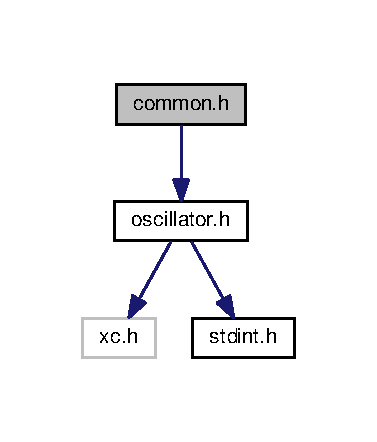
\includegraphics[width=181pt]{common_8h__incl}
\end{center}
\end{figure}
This graph shows which files directly or indirectly include this file\+:\nopagebreak
\begin{figure}[H]
\begin{center}
\leavevmode
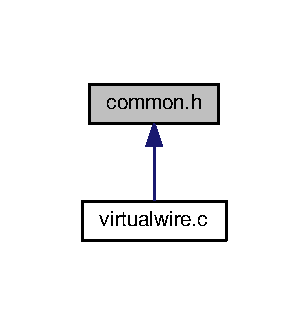
\includegraphics[width=148pt]{common_8h__dep__incl}
\end{center}
\end{figure}
\subsection*{Macros}
\begin{DoxyCompactItemize}
\item 
\#define \hyperlink{common_8h_ab5b48af5b98a9d3afdfef3e7be17819a}{T\+M\+R0\+I\+F}~T0\+I\+F
\item 
\#define \hyperlink{common_8h_aa22ab472cb75f9e7494bf3afbda2de95}{T\+M\+R0\+I\+E}~T0\+I\+E
\end{DoxyCompactItemize}


\subsection{Macro Definition Documentation}
\hypertarget{common_8h_aa22ab472cb75f9e7494bf3afbda2de95}{\index{common.\+h@{common.\+h}!T\+M\+R0\+I\+E@{T\+M\+R0\+I\+E}}
\index{T\+M\+R0\+I\+E@{T\+M\+R0\+I\+E}!common.\+h@{common.\+h}}
\subsubsection[{T\+M\+R0\+I\+E}]{\setlength{\rightskip}{0pt plus 5cm}\#define T\+M\+R0\+I\+E~T0\+I\+E}}\label{common_8h_aa22ab472cb75f9e7494bf3afbda2de95}
\hypertarget{common_8h_ab5b48af5b98a9d3afdfef3e7be17819a}{\index{common.\+h@{common.\+h}!T\+M\+R0\+I\+F@{T\+M\+R0\+I\+F}}
\index{T\+M\+R0\+I\+F@{T\+M\+R0\+I\+F}!common.\+h@{common.\+h}}
\subsubsection[{T\+M\+R0\+I\+F}]{\setlength{\rightskip}{0pt plus 5cm}\#define T\+M\+R0\+I\+F~T0\+I\+F}}\label{common_8h_ab5b48af5b98a9d3afdfef3e7be17819a}
Compatibility with pic16f88 
\hypertarget{crc16_8h}{\section{crc16.\+h File Reference}
\label{crc16_8h}\index{crc16.\+h@{crc16.\+h}}
}
{\ttfamily \#include \char`\"{}stdint.\+h\char`\"{}}\\*
Include dependency graph for crc16.\+h\+:\nopagebreak
\begin{figure}[H]
\begin{center}
\leavevmode
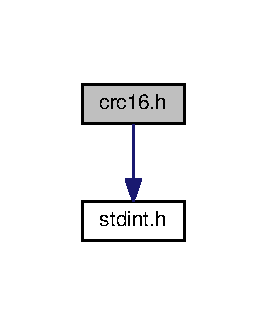
\includegraphics[width=128pt]{crc16_8h__incl}
\end{center}
\end{figure}
This graph shows which files directly or indirectly include this file\+:\nopagebreak
\begin{figure}[H]
\begin{center}
\leavevmode
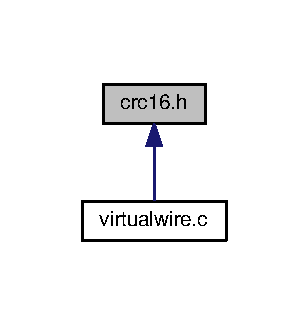
\includegraphics[width=148pt]{crc16_8h__dep__incl}
\end{center}
\end{figure}
\subsection*{Macros}
\begin{DoxyCompactItemize}
\item 
\#define \hyperlink{crc16_8h_a526a4e1347fa25cb82bb0f6e5f4619bf}{lo8}(x)~((x)\&0xff)
\item 
\#define \hyperlink{crc16_8h_a257288eff2b20e6aa2c6ce7bd622f5ec}{hi8}(x)~((x)$>$$>$8)
\end{DoxyCompactItemize}
\subsection*{Functions}
\begin{DoxyCompactItemize}
\item 
\hyperlink{stdint_8h_a1f1825b69244eb3ad2c7165ddc99c956}{uint16\+\_\+t} \hyperlink{crc16_8h_a2a763000bd7d272155103c23a6a0e468}{crc16\+\_\+update} (\hyperlink{stdint_8h_a1f1825b69244eb3ad2c7165ddc99c956}{uint16\+\_\+t} crc, \hyperlink{stdint_8h_aba7bc1797add20fe3efdf37ced1182c5}{uint8\+\_\+t} a)
\item 
\hyperlink{stdint_8h_a1f1825b69244eb3ad2c7165ddc99c956}{uint16\+\_\+t} \hyperlink{crc16_8h_abe3d4804a4bf6a43485c6a6ffcbceb38}{crc\+\_\+xmodem\+\_\+update} (\hyperlink{stdint_8h_a1f1825b69244eb3ad2c7165ddc99c956}{uint16\+\_\+t} crc, \hyperlink{stdint_8h_aba7bc1797add20fe3efdf37ced1182c5}{uint8\+\_\+t} data)
\item 
\hyperlink{stdint_8h_a1f1825b69244eb3ad2c7165ddc99c956}{uint16\+\_\+t} \hyperlink{crc16_8h_a8437443c95668e8cdd921600f1de6c8a}{\+\_\+crc\+\_\+ccitt\+\_\+update} (\hyperlink{stdint_8h_a1f1825b69244eb3ad2c7165ddc99c956}{uint16\+\_\+t} crc, \hyperlink{stdint_8h_aba7bc1797add20fe3efdf37ced1182c5}{uint8\+\_\+t} data)
\item 
\hyperlink{stdint_8h_aba7bc1797add20fe3efdf37ced1182c5}{uint8\+\_\+t} \hyperlink{crc16_8h_aec4f165fcc4c9472dd43feef68e2bab9}{\+\_\+crc\+\_\+ibutton\+\_\+update} (\hyperlink{stdint_8h_aba7bc1797add20fe3efdf37ced1182c5}{uint8\+\_\+t} crc, \hyperlink{stdint_8h_aba7bc1797add20fe3efdf37ced1182c5}{uint8\+\_\+t} data)
\end{DoxyCompactItemize}


\subsection{Macro Definition Documentation}
\hypertarget{crc16_8h_a257288eff2b20e6aa2c6ce7bd622f5ec}{\index{crc16.\+h@{crc16.\+h}!hi8@{hi8}}
\index{hi8@{hi8}!crc16.\+h@{crc16.\+h}}
\subsubsection[{hi8}]{\setlength{\rightskip}{0pt plus 5cm}\#define hi8(
\begin{DoxyParamCaption}
\item[{}]{x}
\end{DoxyParamCaption}
)~((x)$>$$>$8)}}\label{crc16_8h_a257288eff2b20e6aa2c6ce7bd622f5ec}
\hypertarget{crc16_8h_a526a4e1347fa25cb82bb0f6e5f4619bf}{\index{crc16.\+h@{crc16.\+h}!lo8@{lo8}}
\index{lo8@{lo8}!crc16.\+h@{crc16.\+h}}
\subsubsection[{lo8}]{\setlength{\rightskip}{0pt plus 5cm}\#define lo8(
\begin{DoxyParamCaption}
\item[{}]{x}
\end{DoxyParamCaption}
)~((x)\&0xff)}}\label{crc16_8h_a526a4e1347fa25cb82bb0f6e5f4619bf}


\subsection{Function Documentation}
\hypertarget{crc16_8h_a8437443c95668e8cdd921600f1de6c8a}{\index{crc16.\+h@{crc16.\+h}!\+\_\+crc\+\_\+ccitt\+\_\+update@{\+\_\+crc\+\_\+ccitt\+\_\+update}}
\index{\+\_\+crc\+\_\+ccitt\+\_\+update@{\+\_\+crc\+\_\+ccitt\+\_\+update}!crc16.\+h@{crc16.\+h}}
\subsubsection[{\+\_\+crc\+\_\+ccitt\+\_\+update}]{\setlength{\rightskip}{0pt plus 5cm}{\bf uint16\+\_\+t} \+\_\+crc\+\_\+ccitt\+\_\+update (
\begin{DoxyParamCaption}
\item[{{\bf uint16\+\_\+t}}]{crc, }
\item[{{\bf uint8\+\_\+t}}]{data}
\end{DoxyParamCaption}
)}}\label{crc16_8h_a8437443c95668e8cdd921600f1de6c8a}
\hypertarget{crc16_8h_aec4f165fcc4c9472dd43feef68e2bab9}{\index{crc16.\+h@{crc16.\+h}!\+\_\+crc\+\_\+ibutton\+\_\+update@{\+\_\+crc\+\_\+ibutton\+\_\+update}}
\index{\+\_\+crc\+\_\+ibutton\+\_\+update@{\+\_\+crc\+\_\+ibutton\+\_\+update}!crc16.\+h@{crc16.\+h}}
\subsubsection[{\+\_\+crc\+\_\+ibutton\+\_\+update}]{\setlength{\rightskip}{0pt plus 5cm}{\bf uint8\+\_\+t} \+\_\+crc\+\_\+ibutton\+\_\+update (
\begin{DoxyParamCaption}
\item[{{\bf uint8\+\_\+t}}]{crc, }
\item[{{\bf uint8\+\_\+t}}]{data}
\end{DoxyParamCaption}
)}}\label{crc16_8h_aec4f165fcc4c9472dd43feef68e2bab9}
\hypertarget{crc16_8h_a2a763000bd7d272155103c23a6a0e468}{\index{crc16.\+h@{crc16.\+h}!crc16\+\_\+update@{crc16\+\_\+update}}
\index{crc16\+\_\+update@{crc16\+\_\+update}!crc16.\+h@{crc16.\+h}}
\subsubsection[{crc16\+\_\+update}]{\setlength{\rightskip}{0pt plus 5cm}{\bf uint16\+\_\+t} crc16\+\_\+update (
\begin{DoxyParamCaption}
\item[{{\bf uint16\+\_\+t}}]{crc, }
\item[{{\bf uint8\+\_\+t}}]{a}
\end{DoxyParamCaption}
)}}\label{crc16_8h_a2a763000bd7d272155103c23a6a0e468}
\hypertarget{crc16_8h_abe3d4804a4bf6a43485c6a6ffcbceb38}{\index{crc16.\+h@{crc16.\+h}!crc\+\_\+xmodem\+\_\+update@{crc\+\_\+xmodem\+\_\+update}}
\index{crc\+\_\+xmodem\+\_\+update@{crc\+\_\+xmodem\+\_\+update}!crc16.\+h@{crc16.\+h}}
\subsubsection[{crc\+\_\+xmodem\+\_\+update}]{\setlength{\rightskip}{0pt plus 5cm}{\bf uint16\+\_\+t} crc\+\_\+xmodem\+\_\+update (
\begin{DoxyParamCaption}
\item[{{\bf uint16\+\_\+t}}]{crc, }
\item[{{\bf uint8\+\_\+t}}]{data}
\end{DoxyParamCaption}
)}}\label{crc16_8h_abe3d4804a4bf6a43485c6a6ffcbceb38}

\hypertarget{main_8c}{\section{main.\+c File Reference}
\label{main_8c}\index{main.\+c@{main.\+c}}
}
{\ttfamily \#include $<$xc.\+h$>$}\\*
{\ttfamily \#include $<$stdint.\+h$>$}\\*
{\ttfamily \#include $<$stdio.\+h$>$}\\*
{\ttfamily \#include $<$pic16lf1786.\+h$>$}\\*
{\ttfamily \#include \char`\"{}types.\+h\char`\"{}}\\*
{\ttfamily \#include \char`\"{}timer.\+h\char`\"{}}\\*
{\ttfamily \#include \char`\"{}usart.\+h\char`\"{}}\\*
{\ttfamily \#include \char`\"{}analog.\+h\char`\"{}}\\*
Include dependency graph for main.\+c\+:\nopagebreak
\begin{figure}[H]
\begin{center}
\leavevmode
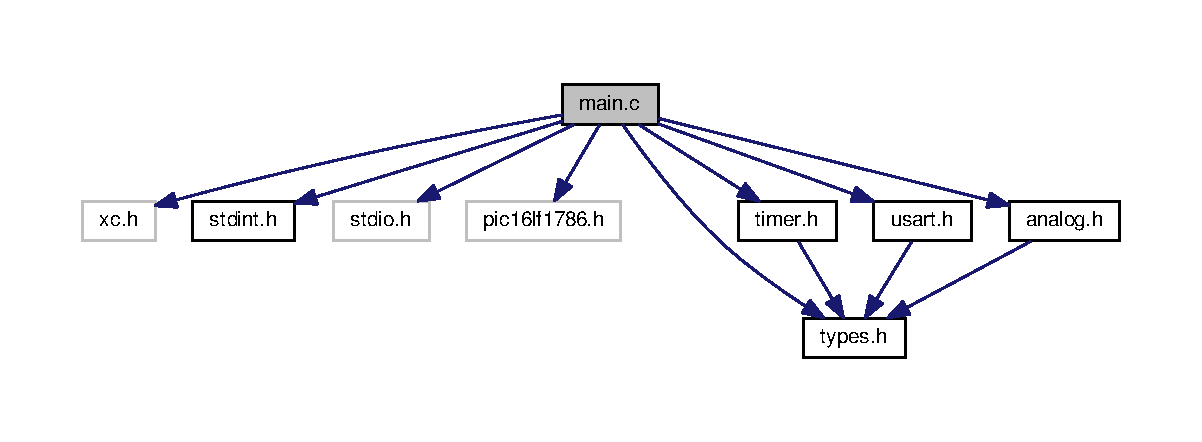
\includegraphics[width=350pt]{main_8c__incl}
\end{center}
\end{figure}
\subsection*{Functions}
\begin{DoxyCompactItemize}
\item 
void interrupt \hyperlink{main_8c_a79a844e55ea6a553355ea812b7f42dda}{isr\+\_\+general} ()
\item 
void \hyperlink{main_8c_a48d0198b93f3ba05a7c2bbf51a2c8aa5}{baby\+\_\+callback} ()
\item 
void \hyperlink{main_8c_a6288eba0f8e8ad3ab1544ad731eb7667}{main} (void)
\end{DoxyCompactItemize}


\subsection{Function Documentation}
\hypertarget{main_8c_a48d0198b93f3ba05a7c2bbf51a2c8aa5}{\index{main.\+c@{main.\+c}!baby\+\_\+callback@{baby\+\_\+callback}}
\index{baby\+\_\+callback@{baby\+\_\+callback}!main.\+c@{main.\+c}}
\subsubsection[{baby\+\_\+callback}]{\setlength{\rightskip}{0pt plus 5cm}void baby\+\_\+callback (
\begin{DoxyParamCaption}
{}
\end{DoxyParamCaption}
)}}\label{main_8c_a48d0198b93f3ba05a7c2bbf51a2c8aa5}
\hypertarget{main_8c_a79a844e55ea6a553355ea812b7f42dda}{\index{main.\+c@{main.\+c}!isr\+\_\+general@{isr\+\_\+general}}
\index{isr\+\_\+general@{isr\+\_\+general}!main.\+c@{main.\+c}}
\subsubsection[{isr\+\_\+general}]{\setlength{\rightskip}{0pt plus 5cm}void interrupt isr\+\_\+general (
\begin{DoxyParamCaption}
{}
\end{DoxyParamCaption}
)}}\label{main_8c_a79a844e55ea6a553355ea812b7f42dda}
Interrupt Service Routine (I\+S\+R) para tratamento de interrup��es geral.

I\+N\+T\+C\+O\+Nbits.\+G\+I\+E vira L\+O\+W quando entra aqui, e H\+I\+G\+H quando sai, automaticamente. \hypertarget{main_8c_a6288eba0f8e8ad3ab1544ad731eb7667}{\index{main.\+c@{main.\+c}!main@{main}}
\index{main@{main}!main.\+c@{main.\+c}}
\subsubsection[{main}]{\setlength{\rightskip}{0pt plus 5cm}void main (
\begin{DoxyParamCaption}
\item[{void}]{}
\end{DoxyParamCaption}
)}}\label{main_8c_a6288eba0f8e8ad3ab1544ad731eb7667}

\hypertarget{oscillator_8c}{\section{oscillator.\+c File Reference}
\label{oscillator_8c}\index{oscillator.\+c@{oscillator.\+c}}
}
{\ttfamily \#include $<$pic16lf1786.\+h$>$}\\*
{\ttfamily \#include \char`\"{}oscillator.\+h\char`\"{}}\\*
Include dependency graph for oscillator.\+c\+:\nopagebreak
\begin{figure}[H]
\begin{center}
\leavevmode
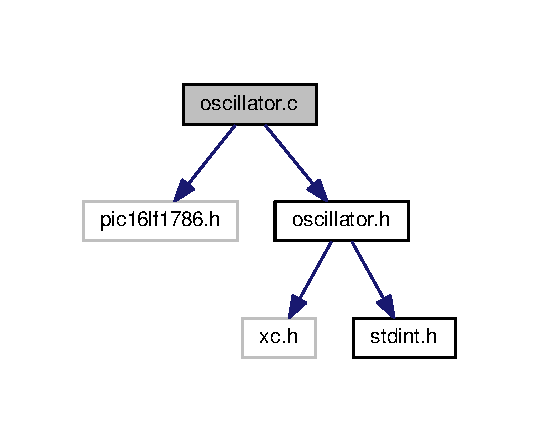
\includegraphics[width=258pt]{oscillator_8c__incl}
\end{center}
\end{figure}
\subsection*{Functions}
\begin{DoxyCompactItemize}
\item 
void \hyperlink{oscillator_8c_a1295413556e7b5b4d7356a50db870b63}{oscillator\+\_\+init\+\_\+internal} ()
\item 
\hyperlink{stdint_8h_a06896e8c53f721507066c079052171f8}{uint32\+\_\+t} \hyperlink{oscillator_8c_a5aff86b3843a834e3ad70e19655c1d04}{oscillator\+\_\+get\+\_\+frequency} ()
\end{DoxyCompactItemize}


\subsection{Function Documentation}
\hypertarget{oscillator_8c_a5aff86b3843a834e3ad70e19655c1d04}{\index{oscillator.\+c@{oscillator.\+c}!oscillator\+\_\+get\+\_\+frequency@{oscillator\+\_\+get\+\_\+frequency}}
\index{oscillator\+\_\+get\+\_\+frequency@{oscillator\+\_\+get\+\_\+frequency}!oscillator.\+c@{oscillator.\+c}}
\subsubsection[{oscillator\+\_\+get\+\_\+frequency}]{\setlength{\rightskip}{0pt plus 5cm}{\bf uint32\+\_\+t} oscillator\+\_\+get\+\_\+frequency (
\begin{DoxyParamCaption}
{}
\end{DoxyParamCaption}
)}}\label{oscillator_8c_a5aff86b3843a834e3ad70e19655c1d04}
\hypertarget{oscillator_8c_a1295413556e7b5b4d7356a50db870b63}{\index{oscillator.\+c@{oscillator.\+c}!oscillator\+\_\+init\+\_\+internal@{oscillator\+\_\+init\+\_\+internal}}
\index{oscillator\+\_\+init\+\_\+internal@{oscillator\+\_\+init\+\_\+internal}!oscillator.\+c@{oscillator.\+c}}
\subsubsection[{oscillator\+\_\+init\+\_\+internal}]{\setlength{\rightskip}{0pt plus 5cm}void oscillator\+\_\+init\+\_\+internal (
\begin{DoxyParamCaption}
{}
\end{DoxyParamCaption}
)}}\label{oscillator_8c_a1295413556e7b5b4d7356a50db870b63}

\hypertarget{oscillator_8h}{\section{oscillator.\+h File Reference}
\label{oscillator_8h}\index{oscillator.\+h@{oscillator.\+h}}
}
{\ttfamily \#include $<$xc.\+h$>$}\\*
{\ttfamily \#include $<$stdint.\+h$>$}\\*
Include dependency graph for oscillator.\+h\+:\nopagebreak
\begin{figure}[H]
\begin{center}
\leavevmode
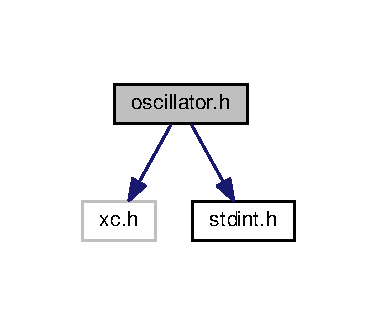
\includegraphics[width=181pt]{oscillator_8h__incl}
\end{center}
\end{figure}
This graph shows which files directly or indirectly include this file\+:\nopagebreak
\begin{figure}[H]
\begin{center}
\leavevmode
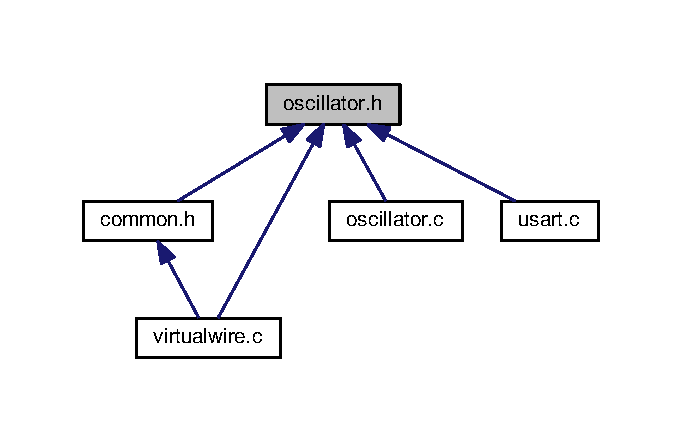
\includegraphics[width=327pt]{oscillator_8h__dep__incl}
\end{center}
\end{figure}
\subsection*{Macros}
\begin{DoxyCompactItemize}
\item 
\#define \hyperlink{oscillator_8h_a37a353f4d28056244ec8f5a0f6026e48}{O\+S\+C\+I\+L\+L\+A\+T\+O\+R\+\_\+\+I\+N\+T\+E\+R\+N\+A\+L\+\_\+\+F\+R\+E\+Q\+U\+E\+N\+C\+Y\+\_\+\+H\+F\+\_\+32\+M\+Hz}~95
\item 
\#define \hyperlink{oscillator_8h_a5c44fe2868be77b0727e1f8f1101d1ef}{O\+S\+C\+I\+L\+L\+A\+T\+O\+R\+\_\+\+I\+N\+T\+E\+R\+N\+A\+L\+\_\+\+F\+R\+E\+Q\+U\+E\+N\+C\+Y\+\_\+\+H\+F\+\_\+16\+M\+Hz}~79
\item 
\#define \hyperlink{oscillator_8h_ace4194ffae45a022e1f00b5427f5eec2}{O\+S\+C\+I\+L\+L\+A\+T\+O\+R\+\_\+\+I\+N\+T\+E\+R\+N\+A\+L\+\_\+\+F\+R\+E\+Q\+U\+E\+N\+C\+Y\+\_\+\+H\+F\+\_\+8\+M\+Hz}~78
\item 
\#define \hyperlink{oscillator_8h_ad5d8c5f66bfc3b43db82a8206e507bd2}{O\+S\+C\+I\+L\+L\+A\+T\+O\+R\+\_\+\+I\+N\+T\+E\+R\+N\+A\+L\+\_\+\+F\+R\+E\+Q\+U\+E\+N\+C\+Y\+\_\+\+H\+F\+\_\+4\+M\+Hz}~77
\item 
\#define \hyperlink{oscillator_8h_ad87f9efce23dac882548b2ef0011ee19}{O\+S\+C\+I\+L\+L\+A\+T\+O\+R\+\_\+\+I\+N\+T\+E\+R\+N\+A\+L\+\_\+\+F\+R\+E\+Q\+U\+E\+N\+C\+Y\+\_\+\+H\+F\+\_\+2\+M\+Hz}~76
\item 
\#define \hyperlink{oscillator_8h_ae5d441624571f856235ec9fa1436b793}{O\+S\+C\+I\+L\+L\+A\+T\+O\+R\+\_\+\+I\+N\+T\+E\+R\+N\+A\+L\+\_\+\+F\+R\+E\+Q\+U\+E\+N\+C\+Y\+\_\+\+H\+F\+\_\+1\+M\+Hz}~75
\item 
\#define \hyperlink{oscillator_8h_a583b1b31a1ada4428710ab2016f7f84b}{O\+S\+C\+I\+L\+L\+A\+T\+O\+R\+\_\+\+I\+N\+T\+E\+R\+N\+A\+L\+\_\+\+F\+R\+E\+Q\+U\+E\+N\+C\+Y\+\_\+\+H\+F\+\_\+500k\+Hz}~74
\item 
\#define \hyperlink{oscillator_8h_ae8419c01e754308f956984f8d28785b3}{O\+S\+C\+I\+L\+L\+A\+T\+O\+R\+\_\+\+I\+N\+T\+E\+R\+N\+A\+L\+\_\+\+F\+R\+E\+Q\+U\+E\+N\+C\+Y\+\_\+\+H\+F\+\_\+250k\+Hz}~73
\item 
\#define \hyperlink{oscillator_8h_a02607ff0f63681c218bedbbc6ae98a51}{O\+S\+C\+I\+L\+L\+A\+T\+O\+R\+\_\+\+I\+N\+T\+E\+R\+N\+A\+L\+\_\+\+F\+R\+E\+Q\+U\+E\+N\+C\+Y\+\_\+\+H\+F\+\_\+125k\+Hz}~72
\item 
\#define \hyperlink{oscillator_8h_a01a4f519f7b907cc3127714966afa9f0}{O\+S\+C\+I\+L\+L\+A\+T\+O\+R\+\_\+\+I\+N\+T\+E\+R\+N\+A\+L\+\_\+\+F\+R\+E\+Q\+U\+E\+N\+C\+Y\+\_\+\+M\+F\+\_\+500k\+Hz}~39
\item 
\#define \hyperlink{oscillator_8h_a46e0e8075071103c980308d8d165da35}{O\+S\+C\+I\+L\+L\+A\+T\+O\+R\+\_\+\+I\+N\+T\+E\+R\+N\+A\+L\+\_\+\+F\+R\+E\+Q\+U\+E\+N\+C\+Y\+\_\+\+M\+F\+\_\+250k\+Hz}~38
\item 
\#define \hyperlink{oscillator_8h_a5848ddbc61ef4a8957ba7ca6c9d902ce}{O\+S\+C\+I\+L\+L\+A\+T\+O\+R\+\_\+\+I\+N\+T\+E\+R\+N\+A\+L\+\_\+\+F\+R\+E\+Q\+U\+E\+N\+C\+Y\+\_\+\+M\+F\+\_\+125k\+Hz}~37
\item 
\#define \hyperlink{oscillator_8h_a700878ad47002884812a6eb30821015f}{O\+S\+C\+I\+L\+L\+A\+T\+O\+R\+\_\+\+I\+N\+T\+E\+R\+N\+A\+L\+\_\+\+F\+R\+E\+Q\+U\+E\+N\+C\+Y\+\_\+\+M\+F\+\_\+62500\+Hz}~36
\item 
\#define \hyperlink{oscillator_8h_a19406c7bc589ef8ee99aae12d0efe02b}{O\+S\+C\+I\+L\+L\+A\+T\+O\+R\+\_\+\+I\+N\+T\+E\+R\+N\+A\+L\+\_\+\+F\+R\+E\+Q\+U\+E\+N\+C\+Y\+\_\+\+H\+F\+\_\+31250\+Hz}~43
\item 
\#define \hyperlink{oscillator_8h_ae3cbd3eed6599471efde7ffdf90875d6}{O\+S\+C\+I\+L\+L\+A\+T\+O\+R\+\_\+\+I\+N\+T\+E\+R\+N\+A\+L\+\_\+\+F\+R\+E\+Q\+U\+E\+N\+C\+Y\+\_\+\+M\+F\+\_\+31250\+Hz}~22
\item 
\#define \hyperlink{oscillator_8h_aedd7aab6f4977d28f99d796f915b8c14}{O\+S\+C\+I\+L\+L\+A\+T\+O\+R\+\_\+\+I\+N\+T\+E\+R\+N\+A\+L\+\_\+\+F\+R\+E\+Q\+U\+E\+N\+C\+Y\+\_\+\+L\+F\+\_\+31000\+Hz}~0
\item 
\#define \hyperlink{oscillator_8h_a40d930930cfaedd97557320de21f6c62}{O\+S\+C\+I\+L\+L\+A\+T\+O\+R}~\hyperlink{oscillator_8h_ad5d8c5f66bfc3b43db82a8206e507bd2}{O\+S\+C\+I\+L\+L\+A\+T\+O\+R\+\_\+\+I\+N\+T\+E\+R\+N\+A\+L\+\_\+\+F\+R\+E\+Q\+U\+E\+N\+C\+Y\+\_\+\+H\+F\+\_\+4\+M\+Hz}
\item 
\#define \hyperlink{oscillator_8h_a024148e99a7143db044a48216664d03d}{\+\_\+\+X\+T\+A\+L\+\_\+\+F\+R\+E\+Q}~4000000
\end{DoxyCompactItemize}
\subsection*{Functions}
\begin{DoxyCompactItemize}
\item 
void \hyperlink{oscillator_8h_a1295413556e7b5b4d7356a50db870b63}{oscillator\+\_\+init\+\_\+internal} ()
\item 
\hyperlink{stdint_8h_a06896e8c53f721507066c079052171f8}{uint32\+\_\+t} \hyperlink{oscillator_8h_a5aff86b3843a834e3ad70e19655c1d04}{oscillator\+\_\+get\+\_\+frequency} ()
\end{DoxyCompactItemize}


\subsection{Macro Definition Documentation}
\hypertarget{oscillator_8h_a024148e99a7143db044a48216664d03d}{\index{oscillator.\+h@{oscillator.\+h}!\+\_\+\+X\+T\+A\+L\+\_\+\+F\+R\+E\+Q@{\+\_\+\+X\+T\+A\+L\+\_\+\+F\+R\+E\+Q}}
\index{\+\_\+\+X\+T\+A\+L\+\_\+\+F\+R\+E\+Q@{\+\_\+\+X\+T\+A\+L\+\_\+\+F\+R\+E\+Q}!oscillator.\+h@{oscillator.\+h}}
\subsubsection[{\+\_\+\+X\+T\+A\+L\+\_\+\+F\+R\+E\+Q}]{\setlength{\rightskip}{0pt plus 5cm}\#define \+\_\+\+X\+T\+A\+L\+\_\+\+F\+R\+E\+Q~4000000}}\label{oscillator_8h_a024148e99a7143db044a48216664d03d}
\hypertarget{oscillator_8h_a40d930930cfaedd97557320de21f6c62}{\index{oscillator.\+h@{oscillator.\+h}!O\+S\+C\+I\+L\+L\+A\+T\+O\+R@{O\+S\+C\+I\+L\+L\+A\+T\+O\+R}}
\index{O\+S\+C\+I\+L\+L\+A\+T\+O\+R@{O\+S\+C\+I\+L\+L\+A\+T\+O\+R}!oscillator.\+h@{oscillator.\+h}}
\subsubsection[{O\+S\+C\+I\+L\+L\+A\+T\+O\+R}]{\setlength{\rightskip}{0pt plus 5cm}\#define O\+S\+C\+I\+L\+L\+A\+T\+O\+R~{\bf O\+S\+C\+I\+L\+L\+A\+T\+O\+R\+\_\+\+I\+N\+T\+E\+R\+N\+A\+L\+\_\+\+F\+R\+E\+Q\+U\+E\+N\+C\+Y\+\_\+\+H\+F\+\_\+4\+M\+Hz}}}\label{oscillator_8h_a40d930930cfaedd97557320de21f6c62}
\hypertarget{oscillator_8h_a02607ff0f63681c218bedbbc6ae98a51}{\index{oscillator.\+h@{oscillator.\+h}!O\+S\+C\+I\+L\+L\+A\+T\+O\+R\+\_\+\+I\+N\+T\+E\+R\+N\+A\+L\+\_\+\+F\+R\+E\+Q\+U\+E\+N\+C\+Y\+\_\+\+H\+F\+\_\+125k\+Hz@{O\+S\+C\+I\+L\+L\+A\+T\+O\+R\+\_\+\+I\+N\+T\+E\+R\+N\+A\+L\+\_\+\+F\+R\+E\+Q\+U\+E\+N\+C\+Y\+\_\+\+H\+F\+\_\+125k\+Hz}}
\index{O\+S\+C\+I\+L\+L\+A\+T\+O\+R\+\_\+\+I\+N\+T\+E\+R\+N\+A\+L\+\_\+\+F\+R\+E\+Q\+U\+E\+N\+C\+Y\+\_\+\+H\+F\+\_\+125k\+Hz@{O\+S\+C\+I\+L\+L\+A\+T\+O\+R\+\_\+\+I\+N\+T\+E\+R\+N\+A\+L\+\_\+\+F\+R\+E\+Q\+U\+E\+N\+C\+Y\+\_\+\+H\+F\+\_\+125k\+Hz}!oscillator.\+h@{oscillator.\+h}}
\subsubsection[{O\+S\+C\+I\+L\+L\+A\+T\+O\+R\+\_\+\+I\+N\+T\+E\+R\+N\+A\+L\+\_\+\+F\+R\+E\+Q\+U\+E\+N\+C\+Y\+\_\+\+H\+F\+\_\+125k\+Hz}]{\setlength{\rightskip}{0pt plus 5cm}\#define O\+S\+C\+I\+L\+L\+A\+T\+O\+R\+\_\+\+I\+N\+T\+E\+R\+N\+A\+L\+\_\+\+F\+R\+E\+Q\+U\+E\+N\+C\+Y\+\_\+\+H\+F\+\_\+125k\+Hz~72}}\label{oscillator_8h_a02607ff0f63681c218bedbbc6ae98a51}
\hypertarget{oscillator_8h_a5c44fe2868be77b0727e1f8f1101d1ef}{\index{oscillator.\+h@{oscillator.\+h}!O\+S\+C\+I\+L\+L\+A\+T\+O\+R\+\_\+\+I\+N\+T\+E\+R\+N\+A\+L\+\_\+\+F\+R\+E\+Q\+U\+E\+N\+C\+Y\+\_\+\+H\+F\+\_\+16\+M\+Hz@{O\+S\+C\+I\+L\+L\+A\+T\+O\+R\+\_\+\+I\+N\+T\+E\+R\+N\+A\+L\+\_\+\+F\+R\+E\+Q\+U\+E\+N\+C\+Y\+\_\+\+H\+F\+\_\+16\+M\+Hz}}
\index{O\+S\+C\+I\+L\+L\+A\+T\+O\+R\+\_\+\+I\+N\+T\+E\+R\+N\+A\+L\+\_\+\+F\+R\+E\+Q\+U\+E\+N\+C\+Y\+\_\+\+H\+F\+\_\+16\+M\+Hz@{O\+S\+C\+I\+L\+L\+A\+T\+O\+R\+\_\+\+I\+N\+T\+E\+R\+N\+A\+L\+\_\+\+F\+R\+E\+Q\+U\+E\+N\+C\+Y\+\_\+\+H\+F\+\_\+16\+M\+Hz}!oscillator.\+h@{oscillator.\+h}}
\subsubsection[{O\+S\+C\+I\+L\+L\+A\+T\+O\+R\+\_\+\+I\+N\+T\+E\+R\+N\+A\+L\+\_\+\+F\+R\+E\+Q\+U\+E\+N\+C\+Y\+\_\+\+H\+F\+\_\+16\+M\+Hz}]{\setlength{\rightskip}{0pt plus 5cm}\#define O\+S\+C\+I\+L\+L\+A\+T\+O\+R\+\_\+\+I\+N\+T\+E\+R\+N\+A\+L\+\_\+\+F\+R\+E\+Q\+U\+E\+N\+C\+Y\+\_\+\+H\+F\+\_\+16\+M\+Hz~79}}\label{oscillator_8h_a5c44fe2868be77b0727e1f8f1101d1ef}
\hypertarget{oscillator_8h_ae5d441624571f856235ec9fa1436b793}{\index{oscillator.\+h@{oscillator.\+h}!O\+S\+C\+I\+L\+L\+A\+T\+O\+R\+\_\+\+I\+N\+T\+E\+R\+N\+A\+L\+\_\+\+F\+R\+E\+Q\+U\+E\+N\+C\+Y\+\_\+\+H\+F\+\_\+1\+M\+Hz@{O\+S\+C\+I\+L\+L\+A\+T\+O\+R\+\_\+\+I\+N\+T\+E\+R\+N\+A\+L\+\_\+\+F\+R\+E\+Q\+U\+E\+N\+C\+Y\+\_\+\+H\+F\+\_\+1\+M\+Hz}}
\index{O\+S\+C\+I\+L\+L\+A\+T\+O\+R\+\_\+\+I\+N\+T\+E\+R\+N\+A\+L\+\_\+\+F\+R\+E\+Q\+U\+E\+N\+C\+Y\+\_\+\+H\+F\+\_\+1\+M\+Hz@{O\+S\+C\+I\+L\+L\+A\+T\+O\+R\+\_\+\+I\+N\+T\+E\+R\+N\+A\+L\+\_\+\+F\+R\+E\+Q\+U\+E\+N\+C\+Y\+\_\+\+H\+F\+\_\+1\+M\+Hz}!oscillator.\+h@{oscillator.\+h}}
\subsubsection[{O\+S\+C\+I\+L\+L\+A\+T\+O\+R\+\_\+\+I\+N\+T\+E\+R\+N\+A\+L\+\_\+\+F\+R\+E\+Q\+U\+E\+N\+C\+Y\+\_\+\+H\+F\+\_\+1\+M\+Hz}]{\setlength{\rightskip}{0pt plus 5cm}\#define O\+S\+C\+I\+L\+L\+A\+T\+O\+R\+\_\+\+I\+N\+T\+E\+R\+N\+A\+L\+\_\+\+F\+R\+E\+Q\+U\+E\+N\+C\+Y\+\_\+\+H\+F\+\_\+1\+M\+Hz~75}}\label{oscillator_8h_ae5d441624571f856235ec9fa1436b793}
\hypertarget{oscillator_8h_ae8419c01e754308f956984f8d28785b3}{\index{oscillator.\+h@{oscillator.\+h}!O\+S\+C\+I\+L\+L\+A\+T\+O\+R\+\_\+\+I\+N\+T\+E\+R\+N\+A\+L\+\_\+\+F\+R\+E\+Q\+U\+E\+N\+C\+Y\+\_\+\+H\+F\+\_\+250k\+Hz@{O\+S\+C\+I\+L\+L\+A\+T\+O\+R\+\_\+\+I\+N\+T\+E\+R\+N\+A\+L\+\_\+\+F\+R\+E\+Q\+U\+E\+N\+C\+Y\+\_\+\+H\+F\+\_\+250k\+Hz}}
\index{O\+S\+C\+I\+L\+L\+A\+T\+O\+R\+\_\+\+I\+N\+T\+E\+R\+N\+A\+L\+\_\+\+F\+R\+E\+Q\+U\+E\+N\+C\+Y\+\_\+\+H\+F\+\_\+250k\+Hz@{O\+S\+C\+I\+L\+L\+A\+T\+O\+R\+\_\+\+I\+N\+T\+E\+R\+N\+A\+L\+\_\+\+F\+R\+E\+Q\+U\+E\+N\+C\+Y\+\_\+\+H\+F\+\_\+250k\+Hz}!oscillator.\+h@{oscillator.\+h}}
\subsubsection[{O\+S\+C\+I\+L\+L\+A\+T\+O\+R\+\_\+\+I\+N\+T\+E\+R\+N\+A\+L\+\_\+\+F\+R\+E\+Q\+U\+E\+N\+C\+Y\+\_\+\+H\+F\+\_\+250k\+Hz}]{\setlength{\rightskip}{0pt plus 5cm}\#define O\+S\+C\+I\+L\+L\+A\+T\+O\+R\+\_\+\+I\+N\+T\+E\+R\+N\+A\+L\+\_\+\+F\+R\+E\+Q\+U\+E\+N\+C\+Y\+\_\+\+H\+F\+\_\+250k\+Hz~73}}\label{oscillator_8h_ae8419c01e754308f956984f8d28785b3}
\hypertarget{oscillator_8h_ad87f9efce23dac882548b2ef0011ee19}{\index{oscillator.\+h@{oscillator.\+h}!O\+S\+C\+I\+L\+L\+A\+T\+O\+R\+\_\+\+I\+N\+T\+E\+R\+N\+A\+L\+\_\+\+F\+R\+E\+Q\+U\+E\+N\+C\+Y\+\_\+\+H\+F\+\_\+2\+M\+Hz@{O\+S\+C\+I\+L\+L\+A\+T\+O\+R\+\_\+\+I\+N\+T\+E\+R\+N\+A\+L\+\_\+\+F\+R\+E\+Q\+U\+E\+N\+C\+Y\+\_\+\+H\+F\+\_\+2\+M\+Hz}}
\index{O\+S\+C\+I\+L\+L\+A\+T\+O\+R\+\_\+\+I\+N\+T\+E\+R\+N\+A\+L\+\_\+\+F\+R\+E\+Q\+U\+E\+N\+C\+Y\+\_\+\+H\+F\+\_\+2\+M\+Hz@{O\+S\+C\+I\+L\+L\+A\+T\+O\+R\+\_\+\+I\+N\+T\+E\+R\+N\+A\+L\+\_\+\+F\+R\+E\+Q\+U\+E\+N\+C\+Y\+\_\+\+H\+F\+\_\+2\+M\+Hz}!oscillator.\+h@{oscillator.\+h}}
\subsubsection[{O\+S\+C\+I\+L\+L\+A\+T\+O\+R\+\_\+\+I\+N\+T\+E\+R\+N\+A\+L\+\_\+\+F\+R\+E\+Q\+U\+E\+N\+C\+Y\+\_\+\+H\+F\+\_\+2\+M\+Hz}]{\setlength{\rightskip}{0pt plus 5cm}\#define O\+S\+C\+I\+L\+L\+A\+T\+O\+R\+\_\+\+I\+N\+T\+E\+R\+N\+A\+L\+\_\+\+F\+R\+E\+Q\+U\+E\+N\+C\+Y\+\_\+\+H\+F\+\_\+2\+M\+Hz~76}}\label{oscillator_8h_ad87f9efce23dac882548b2ef0011ee19}
\hypertarget{oscillator_8h_a19406c7bc589ef8ee99aae12d0efe02b}{\index{oscillator.\+h@{oscillator.\+h}!O\+S\+C\+I\+L\+L\+A\+T\+O\+R\+\_\+\+I\+N\+T\+E\+R\+N\+A\+L\+\_\+\+F\+R\+E\+Q\+U\+E\+N\+C\+Y\+\_\+\+H\+F\+\_\+31250\+Hz@{O\+S\+C\+I\+L\+L\+A\+T\+O\+R\+\_\+\+I\+N\+T\+E\+R\+N\+A\+L\+\_\+\+F\+R\+E\+Q\+U\+E\+N\+C\+Y\+\_\+\+H\+F\+\_\+31250\+Hz}}
\index{O\+S\+C\+I\+L\+L\+A\+T\+O\+R\+\_\+\+I\+N\+T\+E\+R\+N\+A\+L\+\_\+\+F\+R\+E\+Q\+U\+E\+N\+C\+Y\+\_\+\+H\+F\+\_\+31250\+Hz@{O\+S\+C\+I\+L\+L\+A\+T\+O\+R\+\_\+\+I\+N\+T\+E\+R\+N\+A\+L\+\_\+\+F\+R\+E\+Q\+U\+E\+N\+C\+Y\+\_\+\+H\+F\+\_\+31250\+Hz}!oscillator.\+h@{oscillator.\+h}}
\subsubsection[{O\+S\+C\+I\+L\+L\+A\+T\+O\+R\+\_\+\+I\+N\+T\+E\+R\+N\+A\+L\+\_\+\+F\+R\+E\+Q\+U\+E\+N\+C\+Y\+\_\+\+H\+F\+\_\+31250\+Hz}]{\setlength{\rightskip}{0pt plus 5cm}\#define O\+S\+C\+I\+L\+L\+A\+T\+O\+R\+\_\+\+I\+N\+T\+E\+R\+N\+A\+L\+\_\+\+F\+R\+E\+Q\+U\+E\+N\+C\+Y\+\_\+\+H\+F\+\_\+31250\+Hz~43}}\label{oscillator_8h_a19406c7bc589ef8ee99aae12d0efe02b}
\hypertarget{oscillator_8h_a37a353f4d28056244ec8f5a0f6026e48}{\index{oscillator.\+h@{oscillator.\+h}!O\+S\+C\+I\+L\+L\+A\+T\+O\+R\+\_\+\+I\+N\+T\+E\+R\+N\+A\+L\+\_\+\+F\+R\+E\+Q\+U\+E\+N\+C\+Y\+\_\+\+H\+F\+\_\+32\+M\+Hz@{O\+S\+C\+I\+L\+L\+A\+T\+O\+R\+\_\+\+I\+N\+T\+E\+R\+N\+A\+L\+\_\+\+F\+R\+E\+Q\+U\+E\+N\+C\+Y\+\_\+\+H\+F\+\_\+32\+M\+Hz}}
\index{O\+S\+C\+I\+L\+L\+A\+T\+O\+R\+\_\+\+I\+N\+T\+E\+R\+N\+A\+L\+\_\+\+F\+R\+E\+Q\+U\+E\+N\+C\+Y\+\_\+\+H\+F\+\_\+32\+M\+Hz@{O\+S\+C\+I\+L\+L\+A\+T\+O\+R\+\_\+\+I\+N\+T\+E\+R\+N\+A\+L\+\_\+\+F\+R\+E\+Q\+U\+E\+N\+C\+Y\+\_\+\+H\+F\+\_\+32\+M\+Hz}!oscillator.\+h@{oscillator.\+h}}
\subsubsection[{O\+S\+C\+I\+L\+L\+A\+T\+O\+R\+\_\+\+I\+N\+T\+E\+R\+N\+A\+L\+\_\+\+F\+R\+E\+Q\+U\+E\+N\+C\+Y\+\_\+\+H\+F\+\_\+32\+M\+Hz}]{\setlength{\rightskip}{0pt plus 5cm}\#define O\+S\+C\+I\+L\+L\+A\+T\+O\+R\+\_\+\+I\+N\+T\+E\+R\+N\+A\+L\+\_\+\+F\+R\+E\+Q\+U\+E\+N\+C\+Y\+\_\+\+H\+F\+\_\+32\+M\+Hz~95}}\label{oscillator_8h_a37a353f4d28056244ec8f5a0f6026e48}
\hypertarget{oscillator_8h_ad5d8c5f66bfc3b43db82a8206e507bd2}{\index{oscillator.\+h@{oscillator.\+h}!O\+S\+C\+I\+L\+L\+A\+T\+O\+R\+\_\+\+I\+N\+T\+E\+R\+N\+A\+L\+\_\+\+F\+R\+E\+Q\+U\+E\+N\+C\+Y\+\_\+\+H\+F\+\_\+4\+M\+Hz@{O\+S\+C\+I\+L\+L\+A\+T\+O\+R\+\_\+\+I\+N\+T\+E\+R\+N\+A\+L\+\_\+\+F\+R\+E\+Q\+U\+E\+N\+C\+Y\+\_\+\+H\+F\+\_\+4\+M\+Hz}}
\index{O\+S\+C\+I\+L\+L\+A\+T\+O\+R\+\_\+\+I\+N\+T\+E\+R\+N\+A\+L\+\_\+\+F\+R\+E\+Q\+U\+E\+N\+C\+Y\+\_\+\+H\+F\+\_\+4\+M\+Hz@{O\+S\+C\+I\+L\+L\+A\+T\+O\+R\+\_\+\+I\+N\+T\+E\+R\+N\+A\+L\+\_\+\+F\+R\+E\+Q\+U\+E\+N\+C\+Y\+\_\+\+H\+F\+\_\+4\+M\+Hz}!oscillator.\+h@{oscillator.\+h}}
\subsubsection[{O\+S\+C\+I\+L\+L\+A\+T\+O\+R\+\_\+\+I\+N\+T\+E\+R\+N\+A\+L\+\_\+\+F\+R\+E\+Q\+U\+E\+N\+C\+Y\+\_\+\+H\+F\+\_\+4\+M\+Hz}]{\setlength{\rightskip}{0pt plus 5cm}\#define O\+S\+C\+I\+L\+L\+A\+T\+O\+R\+\_\+\+I\+N\+T\+E\+R\+N\+A\+L\+\_\+\+F\+R\+E\+Q\+U\+E\+N\+C\+Y\+\_\+\+H\+F\+\_\+4\+M\+Hz~77}}\label{oscillator_8h_ad5d8c5f66bfc3b43db82a8206e507bd2}
\hypertarget{oscillator_8h_a583b1b31a1ada4428710ab2016f7f84b}{\index{oscillator.\+h@{oscillator.\+h}!O\+S\+C\+I\+L\+L\+A\+T\+O\+R\+\_\+\+I\+N\+T\+E\+R\+N\+A\+L\+\_\+\+F\+R\+E\+Q\+U\+E\+N\+C\+Y\+\_\+\+H\+F\+\_\+500k\+Hz@{O\+S\+C\+I\+L\+L\+A\+T\+O\+R\+\_\+\+I\+N\+T\+E\+R\+N\+A\+L\+\_\+\+F\+R\+E\+Q\+U\+E\+N\+C\+Y\+\_\+\+H\+F\+\_\+500k\+Hz}}
\index{O\+S\+C\+I\+L\+L\+A\+T\+O\+R\+\_\+\+I\+N\+T\+E\+R\+N\+A\+L\+\_\+\+F\+R\+E\+Q\+U\+E\+N\+C\+Y\+\_\+\+H\+F\+\_\+500k\+Hz@{O\+S\+C\+I\+L\+L\+A\+T\+O\+R\+\_\+\+I\+N\+T\+E\+R\+N\+A\+L\+\_\+\+F\+R\+E\+Q\+U\+E\+N\+C\+Y\+\_\+\+H\+F\+\_\+500k\+Hz}!oscillator.\+h@{oscillator.\+h}}
\subsubsection[{O\+S\+C\+I\+L\+L\+A\+T\+O\+R\+\_\+\+I\+N\+T\+E\+R\+N\+A\+L\+\_\+\+F\+R\+E\+Q\+U\+E\+N\+C\+Y\+\_\+\+H\+F\+\_\+500k\+Hz}]{\setlength{\rightskip}{0pt plus 5cm}\#define O\+S\+C\+I\+L\+L\+A\+T\+O\+R\+\_\+\+I\+N\+T\+E\+R\+N\+A\+L\+\_\+\+F\+R\+E\+Q\+U\+E\+N\+C\+Y\+\_\+\+H\+F\+\_\+500k\+Hz~74}}\label{oscillator_8h_a583b1b31a1ada4428710ab2016f7f84b}
\hypertarget{oscillator_8h_ace4194ffae45a022e1f00b5427f5eec2}{\index{oscillator.\+h@{oscillator.\+h}!O\+S\+C\+I\+L\+L\+A\+T\+O\+R\+\_\+\+I\+N\+T\+E\+R\+N\+A\+L\+\_\+\+F\+R\+E\+Q\+U\+E\+N\+C\+Y\+\_\+\+H\+F\+\_\+8\+M\+Hz@{O\+S\+C\+I\+L\+L\+A\+T\+O\+R\+\_\+\+I\+N\+T\+E\+R\+N\+A\+L\+\_\+\+F\+R\+E\+Q\+U\+E\+N\+C\+Y\+\_\+\+H\+F\+\_\+8\+M\+Hz}}
\index{O\+S\+C\+I\+L\+L\+A\+T\+O\+R\+\_\+\+I\+N\+T\+E\+R\+N\+A\+L\+\_\+\+F\+R\+E\+Q\+U\+E\+N\+C\+Y\+\_\+\+H\+F\+\_\+8\+M\+Hz@{O\+S\+C\+I\+L\+L\+A\+T\+O\+R\+\_\+\+I\+N\+T\+E\+R\+N\+A\+L\+\_\+\+F\+R\+E\+Q\+U\+E\+N\+C\+Y\+\_\+\+H\+F\+\_\+8\+M\+Hz}!oscillator.\+h@{oscillator.\+h}}
\subsubsection[{O\+S\+C\+I\+L\+L\+A\+T\+O\+R\+\_\+\+I\+N\+T\+E\+R\+N\+A\+L\+\_\+\+F\+R\+E\+Q\+U\+E\+N\+C\+Y\+\_\+\+H\+F\+\_\+8\+M\+Hz}]{\setlength{\rightskip}{0pt plus 5cm}\#define O\+S\+C\+I\+L\+L\+A\+T\+O\+R\+\_\+\+I\+N\+T\+E\+R\+N\+A\+L\+\_\+\+F\+R\+E\+Q\+U\+E\+N\+C\+Y\+\_\+\+H\+F\+\_\+8\+M\+Hz~78}}\label{oscillator_8h_ace4194ffae45a022e1f00b5427f5eec2}
\hypertarget{oscillator_8h_aedd7aab6f4977d28f99d796f915b8c14}{\index{oscillator.\+h@{oscillator.\+h}!O\+S\+C\+I\+L\+L\+A\+T\+O\+R\+\_\+\+I\+N\+T\+E\+R\+N\+A\+L\+\_\+\+F\+R\+E\+Q\+U\+E\+N\+C\+Y\+\_\+\+L\+F\+\_\+31000\+Hz@{O\+S\+C\+I\+L\+L\+A\+T\+O\+R\+\_\+\+I\+N\+T\+E\+R\+N\+A\+L\+\_\+\+F\+R\+E\+Q\+U\+E\+N\+C\+Y\+\_\+\+L\+F\+\_\+31000\+Hz}}
\index{O\+S\+C\+I\+L\+L\+A\+T\+O\+R\+\_\+\+I\+N\+T\+E\+R\+N\+A\+L\+\_\+\+F\+R\+E\+Q\+U\+E\+N\+C\+Y\+\_\+\+L\+F\+\_\+31000\+Hz@{O\+S\+C\+I\+L\+L\+A\+T\+O\+R\+\_\+\+I\+N\+T\+E\+R\+N\+A\+L\+\_\+\+F\+R\+E\+Q\+U\+E\+N\+C\+Y\+\_\+\+L\+F\+\_\+31000\+Hz}!oscillator.\+h@{oscillator.\+h}}
\subsubsection[{O\+S\+C\+I\+L\+L\+A\+T\+O\+R\+\_\+\+I\+N\+T\+E\+R\+N\+A\+L\+\_\+\+F\+R\+E\+Q\+U\+E\+N\+C\+Y\+\_\+\+L\+F\+\_\+31000\+Hz}]{\setlength{\rightskip}{0pt plus 5cm}\#define O\+S\+C\+I\+L\+L\+A\+T\+O\+R\+\_\+\+I\+N\+T\+E\+R\+N\+A\+L\+\_\+\+F\+R\+E\+Q\+U\+E\+N\+C\+Y\+\_\+\+L\+F\+\_\+31000\+Hz~0}}\label{oscillator_8h_aedd7aab6f4977d28f99d796f915b8c14}
\hypertarget{oscillator_8h_a5848ddbc61ef4a8957ba7ca6c9d902ce}{\index{oscillator.\+h@{oscillator.\+h}!O\+S\+C\+I\+L\+L\+A\+T\+O\+R\+\_\+\+I\+N\+T\+E\+R\+N\+A\+L\+\_\+\+F\+R\+E\+Q\+U\+E\+N\+C\+Y\+\_\+\+M\+F\+\_\+125k\+Hz@{O\+S\+C\+I\+L\+L\+A\+T\+O\+R\+\_\+\+I\+N\+T\+E\+R\+N\+A\+L\+\_\+\+F\+R\+E\+Q\+U\+E\+N\+C\+Y\+\_\+\+M\+F\+\_\+125k\+Hz}}
\index{O\+S\+C\+I\+L\+L\+A\+T\+O\+R\+\_\+\+I\+N\+T\+E\+R\+N\+A\+L\+\_\+\+F\+R\+E\+Q\+U\+E\+N\+C\+Y\+\_\+\+M\+F\+\_\+125k\+Hz@{O\+S\+C\+I\+L\+L\+A\+T\+O\+R\+\_\+\+I\+N\+T\+E\+R\+N\+A\+L\+\_\+\+F\+R\+E\+Q\+U\+E\+N\+C\+Y\+\_\+\+M\+F\+\_\+125k\+Hz}!oscillator.\+h@{oscillator.\+h}}
\subsubsection[{O\+S\+C\+I\+L\+L\+A\+T\+O\+R\+\_\+\+I\+N\+T\+E\+R\+N\+A\+L\+\_\+\+F\+R\+E\+Q\+U\+E\+N\+C\+Y\+\_\+\+M\+F\+\_\+125k\+Hz}]{\setlength{\rightskip}{0pt plus 5cm}\#define O\+S\+C\+I\+L\+L\+A\+T\+O\+R\+\_\+\+I\+N\+T\+E\+R\+N\+A\+L\+\_\+\+F\+R\+E\+Q\+U\+E\+N\+C\+Y\+\_\+\+M\+F\+\_\+125k\+Hz~37}}\label{oscillator_8h_a5848ddbc61ef4a8957ba7ca6c9d902ce}
\hypertarget{oscillator_8h_a46e0e8075071103c980308d8d165da35}{\index{oscillator.\+h@{oscillator.\+h}!O\+S\+C\+I\+L\+L\+A\+T\+O\+R\+\_\+\+I\+N\+T\+E\+R\+N\+A\+L\+\_\+\+F\+R\+E\+Q\+U\+E\+N\+C\+Y\+\_\+\+M\+F\+\_\+250k\+Hz@{O\+S\+C\+I\+L\+L\+A\+T\+O\+R\+\_\+\+I\+N\+T\+E\+R\+N\+A\+L\+\_\+\+F\+R\+E\+Q\+U\+E\+N\+C\+Y\+\_\+\+M\+F\+\_\+250k\+Hz}}
\index{O\+S\+C\+I\+L\+L\+A\+T\+O\+R\+\_\+\+I\+N\+T\+E\+R\+N\+A\+L\+\_\+\+F\+R\+E\+Q\+U\+E\+N\+C\+Y\+\_\+\+M\+F\+\_\+250k\+Hz@{O\+S\+C\+I\+L\+L\+A\+T\+O\+R\+\_\+\+I\+N\+T\+E\+R\+N\+A\+L\+\_\+\+F\+R\+E\+Q\+U\+E\+N\+C\+Y\+\_\+\+M\+F\+\_\+250k\+Hz}!oscillator.\+h@{oscillator.\+h}}
\subsubsection[{O\+S\+C\+I\+L\+L\+A\+T\+O\+R\+\_\+\+I\+N\+T\+E\+R\+N\+A\+L\+\_\+\+F\+R\+E\+Q\+U\+E\+N\+C\+Y\+\_\+\+M\+F\+\_\+250k\+Hz}]{\setlength{\rightskip}{0pt plus 5cm}\#define O\+S\+C\+I\+L\+L\+A\+T\+O\+R\+\_\+\+I\+N\+T\+E\+R\+N\+A\+L\+\_\+\+F\+R\+E\+Q\+U\+E\+N\+C\+Y\+\_\+\+M\+F\+\_\+250k\+Hz~38}}\label{oscillator_8h_a46e0e8075071103c980308d8d165da35}
\hypertarget{oscillator_8h_ae3cbd3eed6599471efde7ffdf90875d6}{\index{oscillator.\+h@{oscillator.\+h}!O\+S\+C\+I\+L\+L\+A\+T\+O\+R\+\_\+\+I\+N\+T\+E\+R\+N\+A\+L\+\_\+\+F\+R\+E\+Q\+U\+E\+N\+C\+Y\+\_\+\+M\+F\+\_\+31250\+Hz@{O\+S\+C\+I\+L\+L\+A\+T\+O\+R\+\_\+\+I\+N\+T\+E\+R\+N\+A\+L\+\_\+\+F\+R\+E\+Q\+U\+E\+N\+C\+Y\+\_\+\+M\+F\+\_\+31250\+Hz}}
\index{O\+S\+C\+I\+L\+L\+A\+T\+O\+R\+\_\+\+I\+N\+T\+E\+R\+N\+A\+L\+\_\+\+F\+R\+E\+Q\+U\+E\+N\+C\+Y\+\_\+\+M\+F\+\_\+31250\+Hz@{O\+S\+C\+I\+L\+L\+A\+T\+O\+R\+\_\+\+I\+N\+T\+E\+R\+N\+A\+L\+\_\+\+F\+R\+E\+Q\+U\+E\+N\+C\+Y\+\_\+\+M\+F\+\_\+31250\+Hz}!oscillator.\+h@{oscillator.\+h}}
\subsubsection[{O\+S\+C\+I\+L\+L\+A\+T\+O\+R\+\_\+\+I\+N\+T\+E\+R\+N\+A\+L\+\_\+\+F\+R\+E\+Q\+U\+E\+N\+C\+Y\+\_\+\+M\+F\+\_\+31250\+Hz}]{\setlength{\rightskip}{0pt plus 5cm}\#define O\+S\+C\+I\+L\+L\+A\+T\+O\+R\+\_\+\+I\+N\+T\+E\+R\+N\+A\+L\+\_\+\+F\+R\+E\+Q\+U\+E\+N\+C\+Y\+\_\+\+M\+F\+\_\+31250\+Hz~22}}\label{oscillator_8h_ae3cbd3eed6599471efde7ffdf90875d6}
\hypertarget{oscillator_8h_a01a4f519f7b907cc3127714966afa9f0}{\index{oscillator.\+h@{oscillator.\+h}!O\+S\+C\+I\+L\+L\+A\+T\+O\+R\+\_\+\+I\+N\+T\+E\+R\+N\+A\+L\+\_\+\+F\+R\+E\+Q\+U\+E\+N\+C\+Y\+\_\+\+M\+F\+\_\+500k\+Hz@{O\+S\+C\+I\+L\+L\+A\+T\+O\+R\+\_\+\+I\+N\+T\+E\+R\+N\+A\+L\+\_\+\+F\+R\+E\+Q\+U\+E\+N\+C\+Y\+\_\+\+M\+F\+\_\+500k\+Hz}}
\index{O\+S\+C\+I\+L\+L\+A\+T\+O\+R\+\_\+\+I\+N\+T\+E\+R\+N\+A\+L\+\_\+\+F\+R\+E\+Q\+U\+E\+N\+C\+Y\+\_\+\+M\+F\+\_\+500k\+Hz@{O\+S\+C\+I\+L\+L\+A\+T\+O\+R\+\_\+\+I\+N\+T\+E\+R\+N\+A\+L\+\_\+\+F\+R\+E\+Q\+U\+E\+N\+C\+Y\+\_\+\+M\+F\+\_\+500k\+Hz}!oscillator.\+h@{oscillator.\+h}}
\subsubsection[{O\+S\+C\+I\+L\+L\+A\+T\+O\+R\+\_\+\+I\+N\+T\+E\+R\+N\+A\+L\+\_\+\+F\+R\+E\+Q\+U\+E\+N\+C\+Y\+\_\+\+M\+F\+\_\+500k\+Hz}]{\setlength{\rightskip}{0pt plus 5cm}\#define O\+S\+C\+I\+L\+L\+A\+T\+O\+R\+\_\+\+I\+N\+T\+E\+R\+N\+A\+L\+\_\+\+F\+R\+E\+Q\+U\+E\+N\+C\+Y\+\_\+\+M\+F\+\_\+500k\+Hz~39}}\label{oscillator_8h_a01a4f519f7b907cc3127714966afa9f0}
\hypertarget{oscillator_8h_a700878ad47002884812a6eb30821015f}{\index{oscillator.\+h@{oscillator.\+h}!O\+S\+C\+I\+L\+L\+A\+T\+O\+R\+\_\+\+I\+N\+T\+E\+R\+N\+A\+L\+\_\+\+F\+R\+E\+Q\+U\+E\+N\+C\+Y\+\_\+\+M\+F\+\_\+62500\+Hz@{O\+S\+C\+I\+L\+L\+A\+T\+O\+R\+\_\+\+I\+N\+T\+E\+R\+N\+A\+L\+\_\+\+F\+R\+E\+Q\+U\+E\+N\+C\+Y\+\_\+\+M\+F\+\_\+62500\+Hz}}
\index{O\+S\+C\+I\+L\+L\+A\+T\+O\+R\+\_\+\+I\+N\+T\+E\+R\+N\+A\+L\+\_\+\+F\+R\+E\+Q\+U\+E\+N\+C\+Y\+\_\+\+M\+F\+\_\+62500\+Hz@{O\+S\+C\+I\+L\+L\+A\+T\+O\+R\+\_\+\+I\+N\+T\+E\+R\+N\+A\+L\+\_\+\+F\+R\+E\+Q\+U\+E\+N\+C\+Y\+\_\+\+M\+F\+\_\+62500\+Hz}!oscillator.\+h@{oscillator.\+h}}
\subsubsection[{O\+S\+C\+I\+L\+L\+A\+T\+O\+R\+\_\+\+I\+N\+T\+E\+R\+N\+A\+L\+\_\+\+F\+R\+E\+Q\+U\+E\+N\+C\+Y\+\_\+\+M\+F\+\_\+62500\+Hz}]{\setlength{\rightskip}{0pt plus 5cm}\#define O\+S\+C\+I\+L\+L\+A\+T\+O\+R\+\_\+\+I\+N\+T\+E\+R\+N\+A\+L\+\_\+\+F\+R\+E\+Q\+U\+E\+N\+C\+Y\+\_\+\+M\+F\+\_\+62500\+Hz~36}}\label{oscillator_8h_a700878ad47002884812a6eb30821015f}


\subsection{Function Documentation}
\hypertarget{oscillator_8h_a5aff86b3843a834e3ad70e19655c1d04}{\index{oscillator.\+h@{oscillator.\+h}!oscillator\+\_\+get\+\_\+frequency@{oscillator\+\_\+get\+\_\+frequency}}
\index{oscillator\+\_\+get\+\_\+frequency@{oscillator\+\_\+get\+\_\+frequency}!oscillator.\+h@{oscillator.\+h}}
\subsubsection[{oscillator\+\_\+get\+\_\+frequency}]{\setlength{\rightskip}{0pt plus 5cm}{\bf uint32\+\_\+t} oscillator\+\_\+get\+\_\+frequency (
\begin{DoxyParamCaption}
{}
\end{DoxyParamCaption}
)}}\label{oscillator_8h_a5aff86b3843a834e3ad70e19655c1d04}
\hypertarget{oscillator_8h_a1295413556e7b5b4d7356a50db870b63}{\index{oscillator.\+h@{oscillator.\+h}!oscillator\+\_\+init\+\_\+internal@{oscillator\+\_\+init\+\_\+internal}}
\index{oscillator\+\_\+init\+\_\+internal@{oscillator\+\_\+init\+\_\+internal}!oscillator.\+h@{oscillator.\+h}}
\subsubsection[{oscillator\+\_\+init\+\_\+internal}]{\setlength{\rightskip}{0pt plus 5cm}void oscillator\+\_\+init\+\_\+internal (
\begin{DoxyParamCaption}
{}
\end{DoxyParamCaption}
)}}\label{oscillator_8h_a1295413556e7b5b4d7356a50db870b63}

\hypertarget{sleep_8c}{\section{sleep.\+c File Reference}
\label{sleep_8c}\index{sleep.\+c@{sleep.\+c}}
}
{\ttfamily \#include \char`\"{}sleep.\+h\char`\"{}}\\*
{\ttfamily \#include $<$xc.\+h$>$}\\*
{\ttfamily \#include $<$pic16lf1786.\+h$>$}\\*
Include dependency graph for sleep.\+c\+:\nopagebreak
\begin{figure}[H]
\begin{center}
\leavevmode
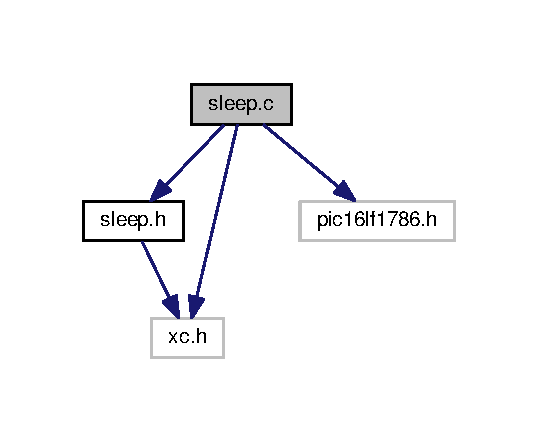
\includegraphics[width=258pt]{sleep_8c__incl}
\end{center}
\end{figure}
\subsection*{Functions}
\begin{DoxyCompactItemize}
\item 
void \hyperlink{sleep_8c_a8469a9105a3b28c76c995ac041f6c07b}{enter\+\_\+deep\+\_\+sleep} ()
\end{DoxyCompactItemize}


\subsection{Function Documentation}
\hypertarget{sleep_8c_a8469a9105a3b28c76c995ac041f6c07b}{\index{sleep.\+c@{sleep.\+c}!enter\+\_\+deep\+\_\+sleep@{enter\+\_\+deep\+\_\+sleep}}
\index{enter\+\_\+deep\+\_\+sleep@{enter\+\_\+deep\+\_\+sleep}!sleep.\+c@{sleep.\+c}}
\subsubsection[{enter\+\_\+deep\+\_\+sleep}]{\setlength{\rightskip}{0pt plus 5cm}void enter\+\_\+deep\+\_\+sleep (
\begin{DoxyParamCaption}
{}
\end{DoxyParamCaption}
)}}\label{sleep_8c_a8469a9105a3b28c76c995ac041f6c07b}

\hypertarget{sleep_8h}{\section{sleep.\+h File Reference}
\label{sleep_8h}\index{sleep.\+h@{sleep.\+h}}
}
{\ttfamily \#include $<$xc.\+h$>$}\\*
Include dependency graph for sleep.\+h\+:\nopagebreak
\begin{figure}[H]
\begin{center}
\leavevmode
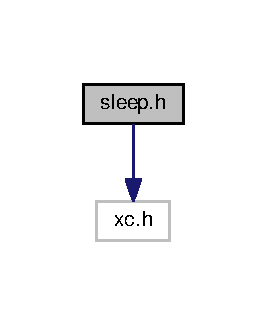
\includegraphics[width=128pt]{sleep_8h__incl}
\end{center}
\end{figure}
This graph shows which files directly or indirectly include this file\+:\nopagebreak
\begin{figure}[H]
\begin{center}
\leavevmode
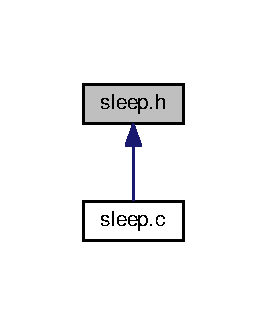
\includegraphics[width=128pt]{sleep_8h__dep__incl}
\end{center}
\end{figure}

\hypertarget{stdint_8h}{\section{stdint.\+h File Reference}
\label{stdint_8h}\index{stdint.\+h@{stdint.\+h}}
}
This graph shows which files directly or indirectly include this file\+:\nopagebreak
\begin{figure}[H]
\begin{center}
\leavevmode
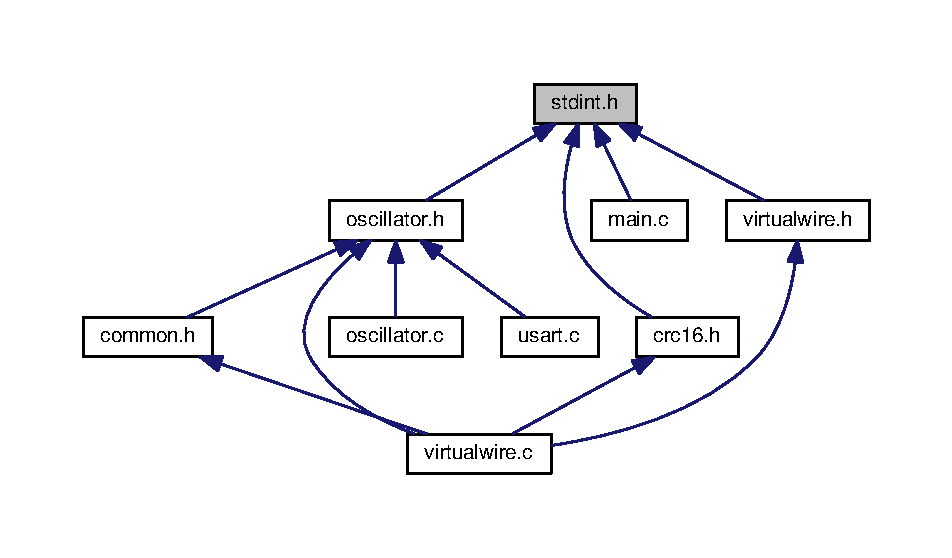
\includegraphics[width=350pt]{stdint_8h__dep__incl}
\end{center}
\end{figure}
\subsection*{Typedefs}
\begin{DoxyCompactItemize}
\item 
typedef char \hyperlink{stdint_8h_ad566f6541e98b74246db1a3a3a85ad49}{int8\+\_\+t}
\item 
typedef int \hyperlink{stdint_8h_ab5525e8f9f02c79fbadd0f03ff724e23}{int16\+\_\+t}
\item 
typedef long \hyperlink{stdint_8h_a0d2e949ab6a1bb62f1b295cc79bc1f60}{int32\+\_\+t}
\item 
typedef unsigned char \hyperlink{stdint_8h_aba7bc1797add20fe3efdf37ced1182c5}{uint8\+\_\+t}
\item 
typedef unsigned int \hyperlink{stdint_8h_a1f1825b69244eb3ad2c7165ddc99c956}{uint16\+\_\+t}
\item 
typedef unsigned long \hyperlink{stdint_8h_a06896e8c53f721507066c079052171f8}{uint32\+\_\+t}
\end{DoxyCompactItemize}


\subsection{Typedef Documentation}
\hypertarget{stdint_8h_ab5525e8f9f02c79fbadd0f03ff724e23}{\index{stdint.\+h@{stdint.\+h}!int16\+\_\+t@{int16\+\_\+t}}
\index{int16\+\_\+t@{int16\+\_\+t}!stdint.\+h@{stdint.\+h}}
\subsubsection[{int16\+\_\+t}]{\setlength{\rightskip}{0pt plus 5cm}typedef int {\bf int16\+\_\+t}}}\label{stdint_8h_ab5525e8f9f02c79fbadd0f03ff724e23}
\hypertarget{stdint_8h_a0d2e949ab6a1bb62f1b295cc79bc1f60}{\index{stdint.\+h@{stdint.\+h}!int32\+\_\+t@{int32\+\_\+t}}
\index{int32\+\_\+t@{int32\+\_\+t}!stdint.\+h@{stdint.\+h}}
\subsubsection[{int32\+\_\+t}]{\setlength{\rightskip}{0pt plus 5cm}typedef long {\bf int32\+\_\+t}}}\label{stdint_8h_a0d2e949ab6a1bb62f1b295cc79bc1f60}
\hypertarget{stdint_8h_ad566f6541e98b74246db1a3a3a85ad49}{\index{stdint.\+h@{stdint.\+h}!int8\+\_\+t@{int8\+\_\+t}}
\index{int8\+\_\+t@{int8\+\_\+t}!stdint.\+h@{stdint.\+h}}
\subsubsection[{int8\+\_\+t}]{\setlength{\rightskip}{0pt plus 5cm}typedef char {\bf int8\+\_\+t}}}\label{stdint_8h_ad566f6541e98b74246db1a3a3a85ad49}
\hypertarget{stdint_8h_a1f1825b69244eb3ad2c7165ddc99c956}{\index{stdint.\+h@{stdint.\+h}!uint16\+\_\+t@{uint16\+\_\+t}}
\index{uint16\+\_\+t@{uint16\+\_\+t}!stdint.\+h@{stdint.\+h}}
\subsubsection[{uint16\+\_\+t}]{\setlength{\rightskip}{0pt plus 5cm}typedef unsigned int {\bf uint16\+\_\+t}}}\label{stdint_8h_a1f1825b69244eb3ad2c7165ddc99c956}
\hypertarget{stdint_8h_a06896e8c53f721507066c079052171f8}{\index{stdint.\+h@{stdint.\+h}!uint32\+\_\+t@{uint32\+\_\+t}}
\index{uint32\+\_\+t@{uint32\+\_\+t}!stdint.\+h@{stdint.\+h}}
\subsubsection[{uint32\+\_\+t}]{\setlength{\rightskip}{0pt plus 5cm}typedef unsigned long {\bf uint32\+\_\+t}}}\label{stdint_8h_a06896e8c53f721507066c079052171f8}
\hypertarget{stdint_8h_aba7bc1797add20fe3efdf37ced1182c5}{\index{stdint.\+h@{stdint.\+h}!uint8\+\_\+t@{uint8\+\_\+t}}
\index{uint8\+\_\+t@{uint8\+\_\+t}!stdint.\+h@{stdint.\+h}}
\subsubsection[{uint8\+\_\+t}]{\setlength{\rightskip}{0pt plus 5cm}typedef unsigned char {\bf uint8\+\_\+t}}}\label{stdint_8h_aba7bc1797add20fe3efdf37ced1182c5}

\hypertarget{string_8h}{\section{string.\+h File Reference}
\label{string_8h}\index{string.\+h@{string.\+h}}
}
This graph shows which files directly or indirectly include this file\+:\nopagebreak
\begin{figure}[H]
\begin{center}
\leavevmode
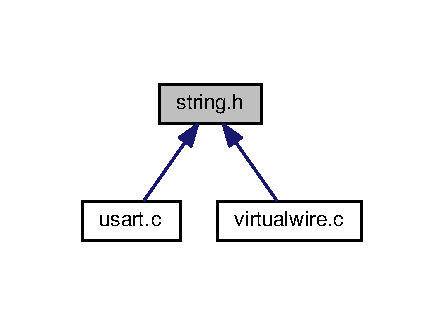
\includegraphics[width=213pt]{string_8h__dep__incl}
\end{center}
\end{figure}
\subsection*{Functions}
\begin{DoxyCompactItemize}
\item 
unsigned char $\ast$ \hyperlink{string_8h_ac648c3aa3f8b879127ecf86cc23347e0}{memcpy} (unsigned char $\ast$dest, unsigned char $\ast$src, unsigned int n)
\end{DoxyCompactItemize}


\subsection{Function Documentation}
\hypertarget{string_8h_ac648c3aa3f8b879127ecf86cc23347e0}{\index{string.\+h@{string.\+h}!memcpy@{memcpy}}
\index{memcpy@{memcpy}!string.\+h@{string.\+h}}
\subsubsection[{memcpy}]{\setlength{\rightskip}{0pt plus 5cm}unsigned char$\ast$ memcpy (
\begin{DoxyParamCaption}
\item[{unsigned char $\ast$}]{dest, }
\item[{unsigned char $\ast$}]{src, }
\item[{unsigned int}]{n}
\end{DoxyParamCaption}
)}}\label{string_8h_ac648c3aa3f8b879127ecf86cc23347e0}

\hypertarget{timer_8c}{\section{timer.\+c File Reference}
\label{timer_8c}\index{timer.\+c@{timer.\+c}}
}
{\ttfamily \#include \char`\"{}timer.\+h\char`\"{}}\\*
{\ttfamily \#include $<$pic16lf1786.\+h$>$}\\*
Include dependency graph for timer.\+c\+:\nopagebreak
\begin{figure}[H]
\begin{center}
\leavevmode
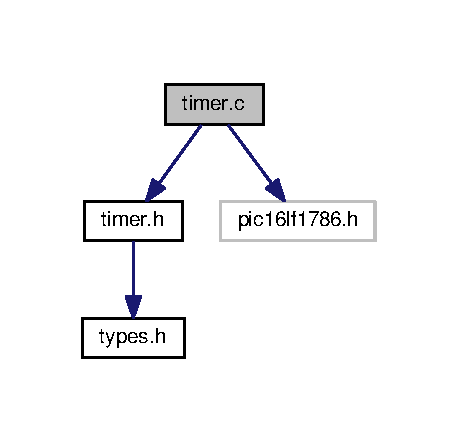
\includegraphics[width=220pt]{timer_8c__incl}
\end{center}
\end{figure}
\subsection*{Functions}
\begin{DoxyCompactItemize}
\item 
void \hyperlink{timer_8c_a76596005fb03c4e47d6b87dcb0fc6014}{timer0\+\_\+start} (\hyperlink{timer_8h_a2ce5e89773b8f9817894c50304932041}{timer0\+\_\+mode\+\_\+t} mode, \hyperlink{timer_8h_a035a5e51eae74c7fe703ec2c8c6521b2}{prescalar\+\_\+use\+\_\+t} prescalar\+\_\+use, \hyperlink{timer_8h_a192cb19cde41f4db80fe3b70dc7c7a3a}{prescalar\+\_\+rate\+\_\+t} prescalar\+\_\+rate, \hyperlink{types_8h_aa8204afb245708cfdad3878a09f1c83e}{callback\+\_\+isr\+\_\+t} timer0\+\_\+callback)
\item 
void \hyperlink{timer_8c_a926ec0c2831f722e965e97e2ccc5d9e3}{timer0\+\_\+isr} ()
\item 
void \hyperlink{timer_8c_ab5cfa68323e2e3176320b4b8e1fb6135}{timer1\+\_\+start} (\hyperlink{timer_8h_a93f45c35f1f1642129e1b6b3ed7cce1f}{timer1\+\_\+mode\+\_\+t} mode, \hyperlink{timer_8h_a7a2c5901c402b8a3c0bf7ea75186946e}{source\+\_\+t1} source, \hyperlink{timer_8h_aaff34f6a035144b2ee97bccb36e40680}{prescalar\+\_\+rate\+\_\+t1} prescaler, \hyperlink{types_8h_aa8204afb245708cfdad3878a09f1c83e}{callback\+\_\+isr\+\_\+t} timer1\+\_\+callback)
\item 
void \hyperlink{timer_8c_ac0dd85f7b03a556f5306aef5032a15f3}{timer1\+\_\+isr} ()
\end{DoxyCompactItemize}
\subsection*{Variables}
\begin{DoxyCompactItemize}
\item 
\hyperlink{types_8h_aa8204afb245708cfdad3878a09f1c83e}{callback\+\_\+isr\+\_\+t} \hyperlink{timer_8c_acdebba0059740c47373a3e8a9b2362fe}{\+\_\+timer0\+\_\+callback} = \hyperlink{types_8h_a070d2ce7b6bb7e5c05602aa8c308d0c4}{N\+U\+L\+L}
\item 
\hyperlink{types_8h_aa8204afb245708cfdad3878a09f1c83e}{callback\+\_\+isr\+\_\+t} \hyperlink{timer_8c_a22fe5ad22625bf0bd7b3bf474c5db142}{\+\_\+timer1\+\_\+callback} = \hyperlink{types_8h_a070d2ce7b6bb7e5c05602aa8c308d0c4}{N\+U\+L\+L}
\end{DoxyCompactItemize}


\subsection{Function Documentation}
\hypertarget{timer_8c_a926ec0c2831f722e965e97e2ccc5d9e3}{\index{timer.\+c@{timer.\+c}!timer0\+\_\+isr@{timer0\+\_\+isr}}
\index{timer0\+\_\+isr@{timer0\+\_\+isr}!timer.\+c@{timer.\+c}}
\subsubsection[{timer0\+\_\+isr}]{\setlength{\rightskip}{0pt plus 5cm}void timer0\+\_\+isr (
\begin{DoxyParamCaption}
{}
\end{DoxyParamCaption}
)}}\label{timer_8c_a926ec0c2831f722e965e97e2ccc5d9e3}
Invoca a rotina associada a interrup��o do timer. \hypertarget{timer_8c_a76596005fb03c4e47d6b87dcb0fc6014}{\index{timer.\+c@{timer.\+c}!timer0\+\_\+start@{timer0\+\_\+start}}
\index{timer0\+\_\+start@{timer0\+\_\+start}!timer.\+c@{timer.\+c}}
\subsubsection[{timer0\+\_\+start}]{\setlength{\rightskip}{0pt plus 5cm}void timer0\+\_\+start (
\begin{DoxyParamCaption}
\item[{{\bf timer0\+\_\+mode\+\_\+t}}]{mode, }
\item[{{\bf prescalar\+\_\+use\+\_\+t}}]{prescalar\+\_\+use, }
\item[{{\bf prescalar\+\_\+rate\+\_\+t}}]{prescalar\+\_\+rate, }
\item[{{\bf callback\+\_\+isr\+\_\+t}}]{timer0\+\_\+isr}
\end{DoxyParamCaption}
)}}\label{timer_8c_a76596005fb03c4e47d6b87dcb0fc6014}

\begin{DoxyParams}{Parameters}
{\em mode} & Modo de execu��o (Timer/\+Counter) \\
\hline
{\em prescalar\+\_\+use} & Usa prescalar de hardware \\
\hline
{\em prescalar\+\_\+rate} & S� � relevante se prescalar\+\_\+use for H\+I\+G\+H. \\
\hline
{\em timer0\+\_\+isr} & rotina executada quando der uma interrup��o. \\
\hline
\end{DoxyParams}
\hypertarget{timer_8c_ac0dd85f7b03a556f5306aef5032a15f3}{\index{timer.\+c@{timer.\+c}!timer1\+\_\+isr@{timer1\+\_\+isr}}
\index{timer1\+\_\+isr@{timer1\+\_\+isr}!timer.\+c@{timer.\+c}}
\subsubsection[{timer1\+\_\+isr}]{\setlength{\rightskip}{0pt plus 5cm}void timer1\+\_\+isr (
\begin{DoxyParamCaption}
{}
\end{DoxyParamCaption}
)}}\label{timer_8c_ac0dd85f7b03a556f5306aef5032a15f3}
\hypertarget{timer_8c_ab5cfa68323e2e3176320b4b8e1fb6135}{\index{timer.\+c@{timer.\+c}!timer1\+\_\+start@{timer1\+\_\+start}}
\index{timer1\+\_\+start@{timer1\+\_\+start}!timer.\+c@{timer.\+c}}
\subsubsection[{timer1\+\_\+start}]{\setlength{\rightskip}{0pt plus 5cm}void timer1\+\_\+start (
\begin{DoxyParamCaption}
\item[{{\bf timer1\+\_\+mode\+\_\+t}}]{mode, }
\item[{{\bf source\+\_\+t1}}]{source, }
\item[{{\bf prescalar\+\_\+rate\+\_\+t1}}]{prescaler, }
\item[{{\bf callback\+\_\+isr\+\_\+t}}]{timer1\+\_\+callback}
\end{DoxyParamCaption}
)}}\label{timer_8c_ab5cfa68323e2e3176320b4b8e1fb6135}
limpa flag vai que ne

habilitar oscilador interno do timer 1

modo contador ou timer 

\subsection{Variable Documentation}
\hypertarget{timer_8c_acdebba0059740c47373a3e8a9b2362fe}{\index{timer.\+c@{timer.\+c}!\+\_\+timer0\+\_\+callback@{\+\_\+timer0\+\_\+callback}}
\index{\+\_\+timer0\+\_\+callback@{\+\_\+timer0\+\_\+callback}!timer.\+c@{timer.\+c}}
\subsubsection[{\+\_\+timer0\+\_\+callback}]{\setlength{\rightskip}{0pt plus 5cm}{\bf callback\+\_\+isr\+\_\+t} \+\_\+timer0\+\_\+callback = {\bf N\+U\+L\+L}}}\label{timer_8c_acdebba0059740c47373a3e8a9b2362fe}
Guarda a referencia para a chamada da fun��o de tratamento de interrup��o do timer. \hypertarget{timer_8c_a22fe5ad22625bf0bd7b3bf474c5db142}{\index{timer.\+c@{timer.\+c}!\+\_\+timer1\+\_\+callback@{\+\_\+timer1\+\_\+callback}}
\index{\+\_\+timer1\+\_\+callback@{\+\_\+timer1\+\_\+callback}!timer.\+c@{timer.\+c}}
\subsubsection[{\+\_\+timer1\+\_\+callback}]{\setlength{\rightskip}{0pt plus 5cm}{\bf callback\+\_\+isr\+\_\+t} \+\_\+timer1\+\_\+callback = {\bf N\+U\+L\+L}}}\label{timer_8c_a22fe5ad22625bf0bd7b3bf474c5db142}

\hypertarget{timer_8h}{\section{timer.\+h File Reference}
\label{timer_8h}\index{timer.\+h@{timer.\+h}}
}
{\ttfamily \#include \char`\"{}types.\+h\char`\"{}}\\*
Include dependency graph for timer.\+h\+:\nopagebreak
\begin{figure}[H]
\begin{center}
\leavevmode
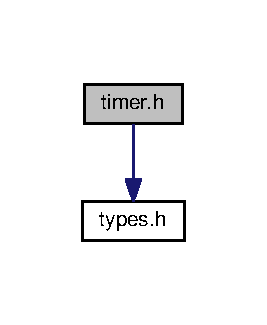
\includegraphics[width=128pt]{timer_8h__incl}
\end{center}
\end{figure}
This graph shows which files directly or indirectly include this file\+:\nopagebreak
\begin{figure}[H]
\begin{center}
\leavevmode
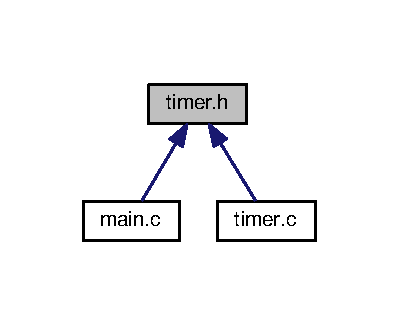
\includegraphics[width=191pt]{timer_8h__dep__incl}
\end{center}
\end{figure}
\subsection*{Enumerations}
\begin{DoxyCompactItemize}
\item 
enum \hyperlink{timer_8h_a2ce5e89773b8f9817894c50304932041}{timer0\+\_\+mode\+\_\+t} \{ \hyperlink{timer_8h_a2ce5e89773b8f9817894c50304932041ad8419716d659ba2d79c6b8d485ea61bc}{T\+I\+M\+E\+R0\+\_\+\+M\+O\+D\+E\+\_\+\+T\+I\+M\+E\+R} = L\+O\+W, 
\hyperlink{timer_8h_a2ce5e89773b8f9817894c50304932041af6b07b51c86a8fce0249757b1adb1eae}{T\+I\+M\+E\+R0\+\_\+\+M\+O\+D\+E\+\_\+\+C\+O\+U\+N\+T\+E\+R} = H\+I\+G\+H
 \}
\item 
enum \hyperlink{timer_8h_a035a5e51eae74c7fe703ec2c8c6521b2}{prescalar\+\_\+use\+\_\+t} \{ \hyperlink{timer_8h_a035a5e51eae74c7fe703ec2c8c6521b2a5c4cfc4ecbf4be28042839fa1957c6ca}{P\+R\+E\+S\+C\+A\+L\+A\+R\+\_\+\+U\+S\+E\+\_\+\+N\+O} = L\+O\+W, 
\hyperlink{timer_8h_a035a5e51eae74c7fe703ec2c8c6521b2abdb6556da7cff2160871e76b43390c81}{P\+R\+E\+S\+C\+A\+L\+A\+R\+\_\+\+U\+S\+E\+\_\+\+Y\+E\+S} = H\+I\+G\+H
 \}
\item 
enum \hyperlink{timer_8h_a192cb19cde41f4db80fe3b70dc7c7a3a}{prescalar\+\_\+rate\+\_\+t} \{ \\*
\hyperlink{timer_8h_a192cb19cde41f4db80fe3b70dc7c7a3aa36b9a5ddd2094f2f9ecb66e68851c37a}{P\+R\+E\+S\+C\+A\+L\+A\+R\+\_\+\+R\+A\+T\+E\+\_\+2} = 0b000, 
\hyperlink{timer_8h_a192cb19cde41f4db80fe3b70dc7c7a3aa25e848b631ecada4fb3add81c7c8d12a}{P\+R\+E\+S\+C\+A\+L\+A\+R\+\_\+\+R\+A\+T\+E\+\_\+4} = 0b001, 
\hyperlink{timer_8h_a192cb19cde41f4db80fe3b70dc7c7a3aab251ec630ffc539dffe59b5b615b3ed4}{P\+R\+E\+S\+C\+A\+L\+A\+R\+\_\+\+R\+A\+T\+E\+\_\+8} = 0b010, 
\hyperlink{timer_8h_a192cb19cde41f4db80fe3b70dc7c7a3aab4ef18a3ddf75bf2945d08d2b22796a7}{P\+R\+E\+S\+C\+A\+L\+A\+R\+\_\+\+R\+A\+T\+E\+\_\+16} = 0b011, 
\\*
\hyperlink{timer_8h_a192cb19cde41f4db80fe3b70dc7c7a3aa30359a49d95cc4657804b4d3ba699ff2}{P\+R\+E\+S\+C\+A\+L\+A\+R\+\_\+\+R\+A\+T\+E\+\_\+32} = 0b100, 
\hyperlink{timer_8h_a192cb19cde41f4db80fe3b70dc7c7a3aa5f59c25a76e8ada4872bb51b7aaf0433}{P\+R\+E\+S\+C\+A\+L\+A\+R\+\_\+\+R\+A\+T\+E\+\_\+64} = 0b001, 
\hyperlink{timer_8h_a192cb19cde41f4db80fe3b70dc7c7a3aa106e4ff2e02a7e012118948829b316e5}{P\+R\+E\+S\+C\+A\+L\+A\+R\+\_\+\+R\+A\+T\+E\+\_\+128} = 0b010, 
\hyperlink{timer_8h_a192cb19cde41f4db80fe3b70dc7c7a3aa27d64dfa99bd612e6859c039f3e75fa9}{P\+R\+E\+S\+C\+A\+L\+A\+R\+\_\+\+R\+A\+T\+E\+\_\+256} = 0b111
 \}
\item 
enum \hyperlink{timer_8h_a93f45c35f1f1642129e1b6b3ed7cce1f}{timer1\+\_\+mode\+\_\+t} \{ \hyperlink{timer_8h_a93f45c35f1f1642129e1b6b3ed7cce1fa4c520dcf1fba4f40b3472b23b8258657}{T\+I\+M\+E\+R1\+\_\+\+M\+O\+D\+E\+\_\+\+T\+I\+M\+E\+R} = L\+O\+W, 
\hyperlink{timer_8h_a93f45c35f1f1642129e1b6b3ed7cce1fa85c596cc404a4d973aab2bcb20c1e060}{T\+I\+M\+E\+R1\+\_\+\+M\+O\+D\+E\+\_\+\+C\+O\+U\+N\+T\+E\+R} = H\+I\+G\+H
 \}
\item 
enum \hyperlink{timer_8h_a7a2c5901c402b8a3c0bf7ea75186946e}{source\+\_\+t1} \{ \hyperlink{timer_8h_a7a2c5901c402b8a3c0bf7ea75186946ea7040b9ad42c2df499298675627e91b49}{T\+I\+M\+E\+R1\+\_\+\+S\+O\+U\+R\+C\+E\+\_\+\+L\+F\+I\+N\+T\+O\+S\+C} = 0b11, 
\hyperlink{timer_8h_a7a2c5901c402b8a3c0bf7ea75186946eae0898257f9fede5625f056f435ce28b4}{T\+I\+M\+E\+R1\+\_\+\+S\+O\+U\+R\+C\+E\+\_\+\+S\+Y\+S\+C\+L\+O\+C\+K} = 0b01, 
\hyperlink{timer_8h_a7a2c5901c402b8a3c0bf7ea75186946eacfad73e3dddc27542cb955d1fe58e0e8}{T\+I\+M\+E\+R1\+\_\+\+S\+O\+U\+R\+C\+E\+\_\+\+S\+Y\+S\+L\+O\+C\+K4} = 0b00, 
\hyperlink{timer_8h_a7a2c5901c402b8a3c0bf7ea75186946ea2aa7b4afbd74480ddfd5c626bff8bc21}{T\+I\+M\+E\+R1\+\_\+\+S\+O\+U\+R\+C\+E\+\_\+\+E\+X\+T\+E\+R\+N\+A\+L} = 0b10
 \}
\item 
enum \hyperlink{timer_8h_aaff34f6a035144b2ee97bccb36e40680}{prescalar\+\_\+rate\+\_\+t1} \{ \hyperlink{timer_8h_aaff34f6a035144b2ee97bccb36e40680a46c196e3a899f3be18f89c20e212ac0b}{P\+R\+E\+S\+C\+A\+L\+A\+R\+T1\+\_\+\+R\+A\+T\+E\+\_\+1} = 0b00, 
\hyperlink{timer_8h_aaff34f6a035144b2ee97bccb36e40680aa8ee0434c25702e7c6d381b2696d20d4}{P\+R\+E\+S\+C\+A\+L\+A\+R\+T1\+\_\+\+R\+A\+T\+E\+\_\+2} = 0b01, 
\hyperlink{timer_8h_aaff34f6a035144b2ee97bccb36e40680ab7fc296021fb9c6b6c6c65eb2742e1b4}{P\+R\+E\+S\+C\+A\+L\+A\+R\+T1\+\_\+\+R\+A\+T\+E\+\_\+4} = 0b10, 
\hyperlink{timer_8h_aaff34f6a035144b2ee97bccb36e40680adc43c9f8df76d593402f371ba7e65fda}{P\+R\+E\+S\+C\+A\+L\+A\+R\+T1\+\_\+\+R\+A\+T\+E\+\_\+8} = 0b11
 \}
\end{DoxyCompactItemize}
\subsection*{Functions}
\begin{DoxyCompactItemize}
\item 
void \hyperlink{timer_8h_a7e9085eb6625d2212f76477f4da0dd47}{timer0\+\_\+start} (\hyperlink{timer_8h_a2ce5e89773b8f9817894c50304932041}{timer0\+\_\+mode\+\_\+t} mode, \hyperlink{timer_8h_a035a5e51eae74c7fe703ec2c8c6521b2}{prescalar\+\_\+use\+\_\+t} prescalar\+\_\+use, \hyperlink{timer_8h_a192cb19cde41f4db80fe3b70dc7c7a3a}{prescalar\+\_\+rate\+\_\+t} prescalar\+\_\+rate, \hyperlink{types_8h_aa8204afb245708cfdad3878a09f1c83e}{callback\+\_\+isr\+\_\+t} \hyperlink{timer_8h_a926ec0c2831f722e965e97e2ccc5d9e3}{timer0\+\_\+isr})
\item 
void \hyperlink{timer_8h_a475e12b70fd380ab4d929a4f3207430c}{timer1\+\_\+start} (\hyperlink{timer_8h_a93f45c35f1f1642129e1b6b3ed7cce1f}{timer1\+\_\+mode\+\_\+t} mode, \hyperlink{timer_8h_a7a2c5901c402b8a3c0bf7ea75186946e}{source\+\_\+t1} source, \hyperlink{timer_8h_aaff34f6a035144b2ee97bccb36e40680}{prescalar\+\_\+rate\+\_\+t1} prescaler, \hyperlink{types_8h_aa8204afb245708cfdad3878a09f1c83e}{callback\+\_\+isr\+\_\+t} \hyperlink{timer_8h_ac0dd85f7b03a556f5306aef5032a15f3}{timer1\+\_\+isr})
\item 
void \hyperlink{timer_8h_a926ec0c2831f722e965e97e2ccc5d9e3}{timer0\+\_\+isr} ()
\item 
void \hyperlink{timer_8h_ac0dd85f7b03a556f5306aef5032a15f3}{timer1\+\_\+isr} ()
\end{DoxyCompactItemize}


\subsection{Enumeration Type Documentation}
\hypertarget{timer_8h_a192cb19cde41f4db80fe3b70dc7c7a3a}{\index{timer.\+h@{timer.\+h}!prescalar\+\_\+rate\+\_\+t@{prescalar\+\_\+rate\+\_\+t}}
\index{prescalar\+\_\+rate\+\_\+t@{prescalar\+\_\+rate\+\_\+t}!timer.\+h@{timer.\+h}}
\subsubsection[{prescalar\+\_\+rate\+\_\+t}]{\setlength{\rightskip}{0pt plus 5cm}enum {\bf prescalar\+\_\+rate\+\_\+t}}}\label{timer_8h_a192cb19cde41f4db80fe3b70dc7c7a3a}
\begin{Desc}
\item[Enumerator]\par
\begin{description}
\index{P\+R\+E\+S\+C\+A\+L\+A\+R\+\_\+\+R\+A\+T\+E\+\_\+2@{P\+R\+E\+S\+C\+A\+L\+A\+R\+\_\+\+R\+A\+T\+E\+\_\+2}!timer.\+h@{timer.\+h}}\index{timer.\+h@{timer.\+h}!P\+R\+E\+S\+C\+A\+L\+A\+R\+\_\+\+R\+A\+T\+E\+\_\+2@{P\+R\+E\+S\+C\+A\+L\+A\+R\+\_\+\+R\+A\+T\+E\+\_\+2}}\item[{\em 
\hypertarget{timer_8h_a192cb19cde41f4db80fe3b70dc7c7a3aa36b9a5ddd2094f2f9ecb66e68851c37a}{P\+R\+E\+S\+C\+A\+L\+A\+R\+\_\+\+R\+A\+T\+E\+\_\+2}\label{timer_8h_a192cb19cde41f4db80fe3b70dc7c7a3aa36b9a5ddd2094f2f9ecb66e68851c37a}
}]\index{P\+R\+E\+S\+C\+A\+L\+A\+R\+\_\+\+R\+A\+T\+E\+\_\+4@{P\+R\+E\+S\+C\+A\+L\+A\+R\+\_\+\+R\+A\+T\+E\+\_\+4}!timer.\+h@{timer.\+h}}\index{timer.\+h@{timer.\+h}!P\+R\+E\+S\+C\+A\+L\+A\+R\+\_\+\+R\+A\+T\+E\+\_\+4@{P\+R\+E\+S\+C\+A\+L\+A\+R\+\_\+\+R\+A\+T\+E\+\_\+4}}\item[{\em 
\hypertarget{timer_8h_a192cb19cde41f4db80fe3b70dc7c7a3aa25e848b631ecada4fb3add81c7c8d12a}{P\+R\+E\+S\+C\+A\+L\+A\+R\+\_\+\+R\+A\+T\+E\+\_\+4}\label{timer_8h_a192cb19cde41f4db80fe3b70dc7c7a3aa25e848b631ecada4fb3add81c7c8d12a}
}]\index{P\+R\+E\+S\+C\+A\+L\+A\+R\+\_\+\+R\+A\+T\+E\+\_\+8@{P\+R\+E\+S\+C\+A\+L\+A\+R\+\_\+\+R\+A\+T\+E\+\_\+8}!timer.\+h@{timer.\+h}}\index{timer.\+h@{timer.\+h}!P\+R\+E\+S\+C\+A\+L\+A\+R\+\_\+\+R\+A\+T\+E\+\_\+8@{P\+R\+E\+S\+C\+A\+L\+A\+R\+\_\+\+R\+A\+T\+E\+\_\+8}}\item[{\em 
\hypertarget{timer_8h_a192cb19cde41f4db80fe3b70dc7c7a3aab251ec630ffc539dffe59b5b615b3ed4}{P\+R\+E\+S\+C\+A\+L\+A\+R\+\_\+\+R\+A\+T\+E\+\_\+8}\label{timer_8h_a192cb19cde41f4db80fe3b70dc7c7a3aab251ec630ffc539dffe59b5b615b3ed4}
}]\index{P\+R\+E\+S\+C\+A\+L\+A\+R\+\_\+\+R\+A\+T\+E\+\_\+16@{P\+R\+E\+S\+C\+A\+L\+A\+R\+\_\+\+R\+A\+T\+E\+\_\+16}!timer.\+h@{timer.\+h}}\index{timer.\+h@{timer.\+h}!P\+R\+E\+S\+C\+A\+L\+A\+R\+\_\+\+R\+A\+T\+E\+\_\+16@{P\+R\+E\+S\+C\+A\+L\+A\+R\+\_\+\+R\+A\+T\+E\+\_\+16}}\item[{\em 
\hypertarget{timer_8h_a192cb19cde41f4db80fe3b70dc7c7a3aab4ef18a3ddf75bf2945d08d2b22796a7}{P\+R\+E\+S\+C\+A\+L\+A\+R\+\_\+\+R\+A\+T\+E\+\_\+16}\label{timer_8h_a192cb19cde41f4db80fe3b70dc7c7a3aab4ef18a3ddf75bf2945d08d2b22796a7}
}]\index{P\+R\+E\+S\+C\+A\+L\+A\+R\+\_\+\+R\+A\+T\+E\+\_\+32@{P\+R\+E\+S\+C\+A\+L\+A\+R\+\_\+\+R\+A\+T\+E\+\_\+32}!timer.\+h@{timer.\+h}}\index{timer.\+h@{timer.\+h}!P\+R\+E\+S\+C\+A\+L\+A\+R\+\_\+\+R\+A\+T\+E\+\_\+32@{P\+R\+E\+S\+C\+A\+L\+A\+R\+\_\+\+R\+A\+T\+E\+\_\+32}}\item[{\em 
\hypertarget{timer_8h_a192cb19cde41f4db80fe3b70dc7c7a3aa30359a49d95cc4657804b4d3ba699ff2}{P\+R\+E\+S\+C\+A\+L\+A\+R\+\_\+\+R\+A\+T\+E\+\_\+32}\label{timer_8h_a192cb19cde41f4db80fe3b70dc7c7a3aa30359a49d95cc4657804b4d3ba699ff2}
}]\index{P\+R\+E\+S\+C\+A\+L\+A\+R\+\_\+\+R\+A\+T\+E\+\_\+64@{P\+R\+E\+S\+C\+A\+L\+A\+R\+\_\+\+R\+A\+T\+E\+\_\+64}!timer.\+h@{timer.\+h}}\index{timer.\+h@{timer.\+h}!P\+R\+E\+S\+C\+A\+L\+A\+R\+\_\+\+R\+A\+T\+E\+\_\+64@{P\+R\+E\+S\+C\+A\+L\+A\+R\+\_\+\+R\+A\+T\+E\+\_\+64}}\item[{\em 
\hypertarget{timer_8h_a192cb19cde41f4db80fe3b70dc7c7a3aa5f59c25a76e8ada4872bb51b7aaf0433}{P\+R\+E\+S\+C\+A\+L\+A\+R\+\_\+\+R\+A\+T\+E\+\_\+64}\label{timer_8h_a192cb19cde41f4db80fe3b70dc7c7a3aa5f59c25a76e8ada4872bb51b7aaf0433}
}]\index{P\+R\+E\+S\+C\+A\+L\+A\+R\+\_\+\+R\+A\+T\+E\+\_\+128@{P\+R\+E\+S\+C\+A\+L\+A\+R\+\_\+\+R\+A\+T\+E\+\_\+128}!timer.\+h@{timer.\+h}}\index{timer.\+h@{timer.\+h}!P\+R\+E\+S\+C\+A\+L\+A\+R\+\_\+\+R\+A\+T\+E\+\_\+128@{P\+R\+E\+S\+C\+A\+L\+A\+R\+\_\+\+R\+A\+T\+E\+\_\+128}}\item[{\em 
\hypertarget{timer_8h_a192cb19cde41f4db80fe3b70dc7c7a3aa106e4ff2e02a7e012118948829b316e5}{P\+R\+E\+S\+C\+A\+L\+A\+R\+\_\+\+R\+A\+T\+E\+\_\+128}\label{timer_8h_a192cb19cde41f4db80fe3b70dc7c7a3aa106e4ff2e02a7e012118948829b316e5}
}]\index{P\+R\+E\+S\+C\+A\+L\+A\+R\+\_\+\+R\+A\+T\+E\+\_\+256@{P\+R\+E\+S\+C\+A\+L\+A\+R\+\_\+\+R\+A\+T\+E\+\_\+256}!timer.\+h@{timer.\+h}}\index{timer.\+h@{timer.\+h}!P\+R\+E\+S\+C\+A\+L\+A\+R\+\_\+\+R\+A\+T\+E\+\_\+256@{P\+R\+E\+S\+C\+A\+L\+A\+R\+\_\+\+R\+A\+T\+E\+\_\+256}}\item[{\em 
\hypertarget{timer_8h_a192cb19cde41f4db80fe3b70dc7c7a3aa27d64dfa99bd612e6859c039f3e75fa9}{P\+R\+E\+S\+C\+A\+L\+A\+R\+\_\+\+R\+A\+T\+E\+\_\+256}\label{timer_8h_a192cb19cde41f4db80fe3b70dc7c7a3aa27d64dfa99bd612e6859c039f3e75fa9}
}]\end{description}
\end{Desc}
\hypertarget{timer_8h_aaff34f6a035144b2ee97bccb36e40680}{\index{timer.\+h@{timer.\+h}!prescalar\+\_\+rate\+\_\+t1@{prescalar\+\_\+rate\+\_\+t1}}
\index{prescalar\+\_\+rate\+\_\+t1@{prescalar\+\_\+rate\+\_\+t1}!timer.\+h@{timer.\+h}}
\subsubsection[{prescalar\+\_\+rate\+\_\+t1}]{\setlength{\rightskip}{0pt plus 5cm}enum {\bf prescalar\+\_\+rate\+\_\+t1}}}\label{timer_8h_aaff34f6a035144b2ee97bccb36e40680}
\begin{Desc}
\item[Enumerator]\par
\begin{description}
\index{P\+R\+E\+S\+C\+A\+L\+A\+R\+T1\+\_\+\+R\+A\+T\+E\+\_\+1@{P\+R\+E\+S\+C\+A\+L\+A\+R\+T1\+\_\+\+R\+A\+T\+E\+\_\+1}!timer.\+h@{timer.\+h}}\index{timer.\+h@{timer.\+h}!P\+R\+E\+S\+C\+A\+L\+A\+R\+T1\+\_\+\+R\+A\+T\+E\+\_\+1@{P\+R\+E\+S\+C\+A\+L\+A\+R\+T1\+\_\+\+R\+A\+T\+E\+\_\+1}}\item[{\em 
\hypertarget{timer_8h_aaff34f6a035144b2ee97bccb36e40680a46c196e3a899f3be18f89c20e212ac0b}{P\+R\+E\+S\+C\+A\+L\+A\+R\+T1\+\_\+\+R\+A\+T\+E\+\_\+1}\label{timer_8h_aaff34f6a035144b2ee97bccb36e40680a46c196e3a899f3be18f89c20e212ac0b}
}]\index{P\+R\+E\+S\+C\+A\+L\+A\+R\+T1\+\_\+\+R\+A\+T\+E\+\_\+2@{P\+R\+E\+S\+C\+A\+L\+A\+R\+T1\+\_\+\+R\+A\+T\+E\+\_\+2}!timer.\+h@{timer.\+h}}\index{timer.\+h@{timer.\+h}!P\+R\+E\+S\+C\+A\+L\+A\+R\+T1\+\_\+\+R\+A\+T\+E\+\_\+2@{P\+R\+E\+S\+C\+A\+L\+A\+R\+T1\+\_\+\+R\+A\+T\+E\+\_\+2}}\item[{\em 
\hypertarget{timer_8h_aaff34f6a035144b2ee97bccb36e40680aa8ee0434c25702e7c6d381b2696d20d4}{P\+R\+E\+S\+C\+A\+L\+A\+R\+T1\+\_\+\+R\+A\+T\+E\+\_\+2}\label{timer_8h_aaff34f6a035144b2ee97bccb36e40680aa8ee0434c25702e7c6d381b2696d20d4}
}]\index{P\+R\+E\+S\+C\+A\+L\+A\+R\+T1\+\_\+\+R\+A\+T\+E\+\_\+4@{P\+R\+E\+S\+C\+A\+L\+A\+R\+T1\+\_\+\+R\+A\+T\+E\+\_\+4}!timer.\+h@{timer.\+h}}\index{timer.\+h@{timer.\+h}!P\+R\+E\+S\+C\+A\+L\+A\+R\+T1\+\_\+\+R\+A\+T\+E\+\_\+4@{P\+R\+E\+S\+C\+A\+L\+A\+R\+T1\+\_\+\+R\+A\+T\+E\+\_\+4}}\item[{\em 
\hypertarget{timer_8h_aaff34f6a035144b2ee97bccb36e40680ab7fc296021fb9c6b6c6c65eb2742e1b4}{P\+R\+E\+S\+C\+A\+L\+A\+R\+T1\+\_\+\+R\+A\+T\+E\+\_\+4}\label{timer_8h_aaff34f6a035144b2ee97bccb36e40680ab7fc296021fb9c6b6c6c65eb2742e1b4}
}]\index{P\+R\+E\+S\+C\+A\+L\+A\+R\+T1\+\_\+\+R\+A\+T\+E\+\_\+8@{P\+R\+E\+S\+C\+A\+L\+A\+R\+T1\+\_\+\+R\+A\+T\+E\+\_\+8}!timer.\+h@{timer.\+h}}\index{timer.\+h@{timer.\+h}!P\+R\+E\+S\+C\+A\+L\+A\+R\+T1\+\_\+\+R\+A\+T\+E\+\_\+8@{P\+R\+E\+S\+C\+A\+L\+A\+R\+T1\+\_\+\+R\+A\+T\+E\+\_\+8}}\item[{\em 
\hypertarget{timer_8h_aaff34f6a035144b2ee97bccb36e40680adc43c9f8df76d593402f371ba7e65fda}{P\+R\+E\+S\+C\+A\+L\+A\+R\+T1\+\_\+\+R\+A\+T\+E\+\_\+8}\label{timer_8h_aaff34f6a035144b2ee97bccb36e40680adc43c9f8df76d593402f371ba7e65fda}
}]\end{description}
\end{Desc}
\hypertarget{timer_8h_a035a5e51eae74c7fe703ec2c8c6521b2}{\index{timer.\+h@{timer.\+h}!prescalar\+\_\+use\+\_\+t@{prescalar\+\_\+use\+\_\+t}}
\index{prescalar\+\_\+use\+\_\+t@{prescalar\+\_\+use\+\_\+t}!timer.\+h@{timer.\+h}}
\subsubsection[{prescalar\+\_\+use\+\_\+t}]{\setlength{\rightskip}{0pt plus 5cm}enum {\bf prescalar\+\_\+use\+\_\+t}}}\label{timer_8h_a035a5e51eae74c7fe703ec2c8c6521b2}
\begin{Desc}
\item[Enumerator]\par
\begin{description}
\index{P\+R\+E\+S\+C\+A\+L\+A\+R\+\_\+\+U\+S\+E\+\_\+\+N\+O@{P\+R\+E\+S\+C\+A\+L\+A\+R\+\_\+\+U\+S\+E\+\_\+\+N\+O}!timer.\+h@{timer.\+h}}\index{timer.\+h@{timer.\+h}!P\+R\+E\+S\+C\+A\+L\+A\+R\+\_\+\+U\+S\+E\+\_\+\+N\+O@{P\+R\+E\+S\+C\+A\+L\+A\+R\+\_\+\+U\+S\+E\+\_\+\+N\+O}}\item[{\em 
\hypertarget{timer_8h_a035a5e51eae74c7fe703ec2c8c6521b2a5c4cfc4ecbf4be28042839fa1957c6ca}{P\+R\+E\+S\+C\+A\+L\+A\+R\+\_\+\+U\+S\+E\+\_\+\+N\+O}\label{timer_8h_a035a5e51eae74c7fe703ec2c8c6521b2a5c4cfc4ecbf4be28042839fa1957c6ca}
}]\index{P\+R\+E\+S\+C\+A\+L\+A\+R\+\_\+\+U\+S\+E\+\_\+\+Y\+E\+S@{P\+R\+E\+S\+C\+A\+L\+A\+R\+\_\+\+U\+S\+E\+\_\+\+Y\+E\+S}!timer.\+h@{timer.\+h}}\index{timer.\+h@{timer.\+h}!P\+R\+E\+S\+C\+A\+L\+A\+R\+\_\+\+U\+S\+E\+\_\+\+Y\+E\+S@{P\+R\+E\+S\+C\+A\+L\+A\+R\+\_\+\+U\+S\+E\+\_\+\+Y\+E\+S}}\item[{\em 
\hypertarget{timer_8h_a035a5e51eae74c7fe703ec2c8c6521b2abdb6556da7cff2160871e76b43390c81}{P\+R\+E\+S\+C\+A\+L\+A\+R\+\_\+\+U\+S\+E\+\_\+\+Y\+E\+S}\label{timer_8h_a035a5e51eae74c7fe703ec2c8c6521b2abdb6556da7cff2160871e76b43390c81}
}]\end{description}
\end{Desc}
\hypertarget{timer_8h_a7a2c5901c402b8a3c0bf7ea75186946e}{\index{timer.\+h@{timer.\+h}!source\+\_\+t1@{source\+\_\+t1}}
\index{source\+\_\+t1@{source\+\_\+t1}!timer.\+h@{timer.\+h}}
\subsubsection[{source\+\_\+t1}]{\setlength{\rightskip}{0pt plus 5cm}enum {\bf source\+\_\+t1}}}\label{timer_8h_a7a2c5901c402b8a3c0bf7ea75186946e}
\begin{Desc}
\item[Enumerator]\par
\begin{description}
\index{T\+I\+M\+E\+R1\+\_\+\+S\+O\+U\+R\+C\+E\+\_\+\+L\+F\+I\+N\+T\+O\+S\+C@{T\+I\+M\+E\+R1\+\_\+\+S\+O\+U\+R\+C\+E\+\_\+\+L\+F\+I\+N\+T\+O\+S\+C}!timer.\+h@{timer.\+h}}\index{timer.\+h@{timer.\+h}!T\+I\+M\+E\+R1\+\_\+\+S\+O\+U\+R\+C\+E\+\_\+\+L\+F\+I\+N\+T\+O\+S\+C@{T\+I\+M\+E\+R1\+\_\+\+S\+O\+U\+R\+C\+E\+\_\+\+L\+F\+I\+N\+T\+O\+S\+C}}\item[{\em 
\hypertarget{timer_8h_a7a2c5901c402b8a3c0bf7ea75186946ea7040b9ad42c2df499298675627e91b49}{T\+I\+M\+E\+R1\+\_\+\+S\+O\+U\+R\+C\+E\+\_\+\+L\+F\+I\+N\+T\+O\+S\+C}\label{timer_8h_a7a2c5901c402b8a3c0bf7ea75186946ea7040b9ad42c2df499298675627e91b49}
}]\index{T\+I\+M\+E\+R1\+\_\+\+S\+O\+U\+R\+C\+E\+\_\+\+S\+Y\+S\+C\+L\+O\+C\+K@{T\+I\+M\+E\+R1\+\_\+\+S\+O\+U\+R\+C\+E\+\_\+\+S\+Y\+S\+C\+L\+O\+C\+K}!timer.\+h@{timer.\+h}}\index{timer.\+h@{timer.\+h}!T\+I\+M\+E\+R1\+\_\+\+S\+O\+U\+R\+C\+E\+\_\+\+S\+Y\+S\+C\+L\+O\+C\+K@{T\+I\+M\+E\+R1\+\_\+\+S\+O\+U\+R\+C\+E\+\_\+\+S\+Y\+S\+C\+L\+O\+C\+K}}\item[{\em 
\hypertarget{timer_8h_a7a2c5901c402b8a3c0bf7ea75186946eae0898257f9fede5625f056f435ce28b4}{T\+I\+M\+E\+R1\+\_\+\+S\+O\+U\+R\+C\+E\+\_\+\+S\+Y\+S\+C\+L\+O\+C\+K}\label{timer_8h_a7a2c5901c402b8a3c0bf7ea75186946eae0898257f9fede5625f056f435ce28b4}
}]\index{T\+I\+M\+E\+R1\+\_\+\+S\+O\+U\+R\+C\+E\+\_\+\+S\+Y\+S\+L\+O\+C\+K4@{T\+I\+M\+E\+R1\+\_\+\+S\+O\+U\+R\+C\+E\+\_\+\+S\+Y\+S\+L\+O\+C\+K4}!timer.\+h@{timer.\+h}}\index{timer.\+h@{timer.\+h}!T\+I\+M\+E\+R1\+\_\+\+S\+O\+U\+R\+C\+E\+\_\+\+S\+Y\+S\+L\+O\+C\+K4@{T\+I\+M\+E\+R1\+\_\+\+S\+O\+U\+R\+C\+E\+\_\+\+S\+Y\+S\+L\+O\+C\+K4}}\item[{\em 
\hypertarget{timer_8h_a7a2c5901c402b8a3c0bf7ea75186946eacfad73e3dddc27542cb955d1fe58e0e8}{T\+I\+M\+E\+R1\+\_\+\+S\+O\+U\+R\+C\+E\+\_\+\+S\+Y\+S\+L\+O\+C\+K4}\label{timer_8h_a7a2c5901c402b8a3c0bf7ea75186946eacfad73e3dddc27542cb955d1fe58e0e8}
}]\index{T\+I\+M\+E\+R1\+\_\+\+S\+O\+U\+R\+C\+E\+\_\+\+E\+X\+T\+E\+R\+N\+A\+L@{T\+I\+M\+E\+R1\+\_\+\+S\+O\+U\+R\+C\+E\+\_\+\+E\+X\+T\+E\+R\+N\+A\+L}!timer.\+h@{timer.\+h}}\index{timer.\+h@{timer.\+h}!T\+I\+M\+E\+R1\+\_\+\+S\+O\+U\+R\+C\+E\+\_\+\+E\+X\+T\+E\+R\+N\+A\+L@{T\+I\+M\+E\+R1\+\_\+\+S\+O\+U\+R\+C\+E\+\_\+\+E\+X\+T\+E\+R\+N\+A\+L}}\item[{\em 
\hypertarget{timer_8h_a7a2c5901c402b8a3c0bf7ea75186946ea2aa7b4afbd74480ddfd5c626bff8bc21}{T\+I\+M\+E\+R1\+\_\+\+S\+O\+U\+R\+C\+E\+\_\+\+E\+X\+T\+E\+R\+N\+A\+L}\label{timer_8h_a7a2c5901c402b8a3c0bf7ea75186946ea2aa7b4afbd74480ddfd5c626bff8bc21}
}]\end{description}
\end{Desc}
\hypertarget{timer_8h_a2ce5e89773b8f9817894c50304932041}{\index{timer.\+h@{timer.\+h}!timer0\+\_\+mode\+\_\+t@{timer0\+\_\+mode\+\_\+t}}
\index{timer0\+\_\+mode\+\_\+t@{timer0\+\_\+mode\+\_\+t}!timer.\+h@{timer.\+h}}
\subsubsection[{timer0\+\_\+mode\+\_\+t}]{\setlength{\rightskip}{0pt plus 5cm}enum {\bf timer0\+\_\+mode\+\_\+t}}}\label{timer_8h_a2ce5e89773b8f9817894c50304932041}
\begin{Desc}
\item[Enumerator]\par
\begin{description}
\index{T\+I\+M\+E\+R0\+\_\+\+M\+O\+D\+E\+\_\+\+T\+I\+M\+E\+R@{T\+I\+M\+E\+R0\+\_\+\+M\+O\+D\+E\+\_\+\+T\+I\+M\+E\+R}!timer.\+h@{timer.\+h}}\index{timer.\+h@{timer.\+h}!T\+I\+M\+E\+R0\+\_\+\+M\+O\+D\+E\+\_\+\+T\+I\+M\+E\+R@{T\+I\+M\+E\+R0\+\_\+\+M\+O\+D\+E\+\_\+\+T\+I\+M\+E\+R}}\item[{\em 
\hypertarget{timer_8h_a2ce5e89773b8f9817894c50304932041ad8419716d659ba2d79c6b8d485ea61bc}{T\+I\+M\+E\+R0\+\_\+\+M\+O\+D\+E\+\_\+\+T\+I\+M\+E\+R}\label{timer_8h_a2ce5e89773b8f9817894c50304932041ad8419716d659ba2d79c6b8d485ea61bc}
}]\index{T\+I\+M\+E\+R0\+\_\+\+M\+O\+D\+E\+\_\+\+C\+O\+U\+N\+T\+E\+R@{T\+I\+M\+E\+R0\+\_\+\+M\+O\+D\+E\+\_\+\+C\+O\+U\+N\+T\+E\+R}!timer.\+h@{timer.\+h}}\index{timer.\+h@{timer.\+h}!T\+I\+M\+E\+R0\+\_\+\+M\+O\+D\+E\+\_\+\+C\+O\+U\+N\+T\+E\+R@{T\+I\+M\+E\+R0\+\_\+\+M\+O\+D\+E\+\_\+\+C\+O\+U\+N\+T\+E\+R}}\item[{\em 
\hypertarget{timer_8h_a2ce5e89773b8f9817894c50304932041af6b07b51c86a8fce0249757b1adb1eae}{T\+I\+M\+E\+R0\+\_\+\+M\+O\+D\+E\+\_\+\+C\+O\+U\+N\+T\+E\+R}\label{timer_8h_a2ce5e89773b8f9817894c50304932041af6b07b51c86a8fce0249757b1adb1eae}
}]\end{description}
\end{Desc}
\hypertarget{timer_8h_a93f45c35f1f1642129e1b6b3ed7cce1f}{\index{timer.\+h@{timer.\+h}!timer1\+\_\+mode\+\_\+t@{timer1\+\_\+mode\+\_\+t}}
\index{timer1\+\_\+mode\+\_\+t@{timer1\+\_\+mode\+\_\+t}!timer.\+h@{timer.\+h}}
\subsubsection[{timer1\+\_\+mode\+\_\+t}]{\setlength{\rightskip}{0pt plus 5cm}enum {\bf timer1\+\_\+mode\+\_\+t}}}\label{timer_8h_a93f45c35f1f1642129e1b6b3ed7cce1f}
\begin{Desc}
\item[Enumerator]\par
\begin{description}
\index{T\+I\+M\+E\+R1\+\_\+\+M\+O\+D\+E\+\_\+\+T\+I\+M\+E\+R@{T\+I\+M\+E\+R1\+\_\+\+M\+O\+D\+E\+\_\+\+T\+I\+M\+E\+R}!timer.\+h@{timer.\+h}}\index{timer.\+h@{timer.\+h}!T\+I\+M\+E\+R1\+\_\+\+M\+O\+D\+E\+\_\+\+T\+I\+M\+E\+R@{T\+I\+M\+E\+R1\+\_\+\+M\+O\+D\+E\+\_\+\+T\+I\+M\+E\+R}}\item[{\em 
\hypertarget{timer_8h_a93f45c35f1f1642129e1b6b3ed7cce1fa4c520dcf1fba4f40b3472b23b8258657}{T\+I\+M\+E\+R1\+\_\+\+M\+O\+D\+E\+\_\+\+T\+I\+M\+E\+R}\label{timer_8h_a93f45c35f1f1642129e1b6b3ed7cce1fa4c520dcf1fba4f40b3472b23b8258657}
}]\index{T\+I\+M\+E\+R1\+\_\+\+M\+O\+D\+E\+\_\+\+C\+O\+U\+N\+T\+E\+R@{T\+I\+M\+E\+R1\+\_\+\+M\+O\+D\+E\+\_\+\+C\+O\+U\+N\+T\+E\+R}!timer.\+h@{timer.\+h}}\index{timer.\+h@{timer.\+h}!T\+I\+M\+E\+R1\+\_\+\+M\+O\+D\+E\+\_\+\+C\+O\+U\+N\+T\+E\+R@{T\+I\+M\+E\+R1\+\_\+\+M\+O\+D\+E\+\_\+\+C\+O\+U\+N\+T\+E\+R}}\item[{\em 
\hypertarget{timer_8h_a93f45c35f1f1642129e1b6b3ed7cce1fa85c596cc404a4d973aab2bcb20c1e060}{T\+I\+M\+E\+R1\+\_\+\+M\+O\+D\+E\+\_\+\+C\+O\+U\+N\+T\+E\+R}\label{timer_8h_a93f45c35f1f1642129e1b6b3ed7cce1fa85c596cc404a4d973aab2bcb20c1e060}
}]\end{description}
\end{Desc}


\subsection{Function Documentation}
\hypertarget{timer_8h_a926ec0c2831f722e965e97e2ccc5d9e3}{\index{timer.\+h@{timer.\+h}!timer0\+\_\+isr@{timer0\+\_\+isr}}
\index{timer0\+\_\+isr@{timer0\+\_\+isr}!timer.\+h@{timer.\+h}}
\subsubsection[{timer0\+\_\+isr}]{\setlength{\rightskip}{0pt plus 5cm}void timer0\+\_\+isr (
\begin{DoxyParamCaption}
{}
\end{DoxyParamCaption}
)}}\label{timer_8h_a926ec0c2831f722e965e97e2ccc5d9e3}
Invoca a rotina associada a interrup��o do timer. \hypertarget{timer_8h_a7e9085eb6625d2212f76477f4da0dd47}{\index{timer.\+h@{timer.\+h}!timer0\+\_\+start@{timer0\+\_\+start}}
\index{timer0\+\_\+start@{timer0\+\_\+start}!timer.\+h@{timer.\+h}}
\subsubsection[{timer0\+\_\+start}]{\setlength{\rightskip}{0pt plus 5cm}void timer0\+\_\+start (
\begin{DoxyParamCaption}
\item[{{\bf timer0\+\_\+mode\+\_\+t}}]{mode, }
\item[{{\bf prescalar\+\_\+use\+\_\+t}}]{prescalar\+\_\+use, }
\item[{{\bf prescalar\+\_\+rate\+\_\+t}}]{prescalar\+\_\+rate, }
\item[{{\bf callback\+\_\+isr\+\_\+t}}]{timer0\+\_\+isr}
\end{DoxyParamCaption}
)}}\label{timer_8h_a7e9085eb6625d2212f76477f4da0dd47}

\begin{DoxyParams}{Parameters}
{\em mode} & Modo de execu��o (Timer/\+Counter) \\
\hline
{\em prescalar\+\_\+use} & Usa prescalar de hardware \\
\hline
{\em prescalar\+\_\+rate} & S� � relevante se prescalar\+\_\+use for H\+I\+G\+H. \\
\hline
{\em timer0\+\_\+isr} & rotina executada quando der uma interrup��o. \\
\hline
\end{DoxyParams}
\hypertarget{timer_8h_ac0dd85f7b03a556f5306aef5032a15f3}{\index{timer.\+h@{timer.\+h}!timer1\+\_\+isr@{timer1\+\_\+isr}}
\index{timer1\+\_\+isr@{timer1\+\_\+isr}!timer.\+h@{timer.\+h}}
\subsubsection[{timer1\+\_\+isr}]{\setlength{\rightskip}{0pt plus 5cm}void timer1\+\_\+isr (
\begin{DoxyParamCaption}
{}
\end{DoxyParamCaption}
)}}\label{timer_8h_ac0dd85f7b03a556f5306aef5032a15f3}
\hypertarget{timer_8h_a475e12b70fd380ab4d929a4f3207430c}{\index{timer.\+h@{timer.\+h}!timer1\+\_\+start@{timer1\+\_\+start}}
\index{timer1\+\_\+start@{timer1\+\_\+start}!timer.\+h@{timer.\+h}}
\subsubsection[{timer1\+\_\+start}]{\setlength{\rightskip}{0pt plus 5cm}void timer1\+\_\+start (
\begin{DoxyParamCaption}
\item[{{\bf timer1\+\_\+mode\+\_\+t}}]{mode, }
\item[{{\bf source\+\_\+t1}}]{source, }
\item[{{\bf prescalar\+\_\+rate\+\_\+t1}}]{prescaler, }
\item[{{\bf callback\+\_\+isr\+\_\+t}}]{timer1\+\_\+isr}
\end{DoxyParamCaption}
)}}\label{timer_8h_a475e12b70fd380ab4d929a4f3207430c}
limpa flag vai que ne

habilitar oscilador interno do timer 1

modo contador ou timer 
\hypertarget{types_8h}{\section{types.\+h File Reference}
\label{types_8h}\index{types.\+h@{types.\+h}}
}
This graph shows which files directly or indirectly include this file\+:\nopagebreak
\begin{figure}[H]
\begin{center}
\leavevmode
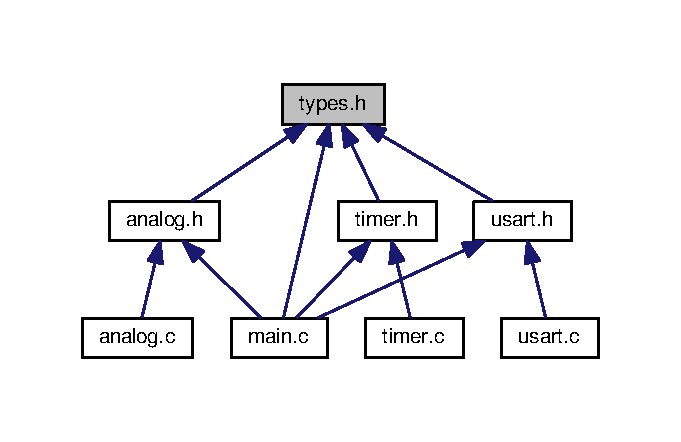
\includegraphics[width=327pt]{types_8h__dep__incl}
\end{center}
\end{figure}
\subsection*{Macros}
\begin{DoxyCompactItemize}
\item 
\#define \hyperlink{types_8h_a070d2ce7b6bb7e5c05602aa8c308d0c4}{N\+U\+L\+L}~((void$\ast$)0)
\item 
\#define \hyperlink{types_8h_a5bb885982ff66a2e0a0a45a8ee9c35e2}{H\+I\+G\+H}~1
\item 
\#define \hyperlink{types_8h_ab811d8c6ff3a505312d3276590444289}{L\+O\+W}~0
\item 
\#define \hyperlink{types_8h_a1bb283bd7893b9855e2f23013891fc82}{I\+N\+P\+U\+T}~\hyperlink{types_8h_a5bb885982ff66a2e0a0a45a8ee9c35e2}{H\+I\+G\+H}
\item 
\#define \hyperlink{types_8h_a61a3c9a18380aafb6e430e79bf596557}{O\+U\+T\+P\+U\+T}~\hyperlink{types_8h_ab811d8c6ff3a505312d3276590444289}{L\+O\+W}
\item 
\#define \hyperlink{types_8h_aa8cecfc5c5c054d2875c03e77b7be15d}{T\+R\+U\+E}~\hyperlink{types_8h_a5bb885982ff66a2e0a0a45a8ee9c35e2}{H\+I\+G\+H}
\item 
\#define \hyperlink{types_8h_aa93f0eb578d23995850d61f7d61c55c1}{F\+A\+L\+S\+E}~\hyperlink{types_8h_ab811d8c6ff3a505312d3276590444289}{L\+O\+W}
\end{DoxyCompactItemize}
\subsection*{Typedefs}
\begin{DoxyCompactItemize}
\item 
typedef unsigned char \hyperlink{types_8h_a0c8186d9b9b7880309c27230bbb5e69d}{byte}
\item 
typedef unsigned char \hyperlink{types_8h_aba7bc1797add20fe3efdf37ced1182c5}{uint8\+\_\+t}
\item 
typedef unsigned int \hyperlink{types_8h_a1f1825b69244eb3ad2c7165ddc99c956}{uint16\+\_\+t}
\item 
typedef unsigned long \hyperlink{types_8h_a06896e8c53f721507066c079052171f8}{uint32\+\_\+t}
\item 
typedef void($\ast$ \hyperlink{types_8h_aa8204afb245708cfdad3878a09f1c83e}{callback\+\_\+isr\+\_\+t} )(void)
\end{DoxyCompactItemize}


\subsection{Macro Definition Documentation}
\hypertarget{types_8h_aa93f0eb578d23995850d61f7d61c55c1}{\index{types.\+h@{types.\+h}!F\+A\+L\+S\+E@{F\+A\+L\+S\+E}}
\index{F\+A\+L\+S\+E@{F\+A\+L\+S\+E}!types.\+h@{types.\+h}}
\subsubsection[{F\+A\+L\+S\+E}]{\setlength{\rightskip}{0pt plus 5cm}\#define F\+A\+L\+S\+E~{\bf L\+O\+W}}}\label{types_8h_aa93f0eb578d23995850d61f7d61c55c1}
Condi��o Booleana para False \hypertarget{types_8h_a5bb885982ff66a2e0a0a45a8ee9c35e2}{\index{types.\+h@{types.\+h}!H\+I\+G\+H@{H\+I\+G\+H}}
\index{H\+I\+G\+H@{H\+I\+G\+H}!types.\+h@{types.\+h}}
\subsubsection[{H\+I\+G\+H}]{\setlength{\rightskip}{0pt plus 5cm}\#define H\+I\+G\+H~1}}\label{types_8h_a5bb885982ff66a2e0a0a45a8ee9c35e2}
Indica quando o estado do bit est� em H\+I\+G\+H ou S\+E\+T \hypertarget{types_8h_a1bb283bd7893b9855e2f23013891fc82}{\index{types.\+h@{types.\+h}!I\+N\+P\+U\+T@{I\+N\+P\+U\+T}}
\index{I\+N\+P\+U\+T@{I\+N\+P\+U\+T}!types.\+h@{types.\+h}}
\subsubsection[{I\+N\+P\+U\+T}]{\setlength{\rightskip}{0pt plus 5cm}\#define I\+N\+P\+U\+T~{\bf H\+I\+G\+H}}}\label{types_8h_a1bb283bd7893b9855e2f23013891fc82}
Indica se o pino ser� de entrada \hypertarget{types_8h_ab811d8c6ff3a505312d3276590444289}{\index{types.\+h@{types.\+h}!L\+O\+W@{L\+O\+W}}
\index{L\+O\+W@{L\+O\+W}!types.\+h@{types.\+h}}
\subsubsection[{L\+O\+W}]{\setlength{\rightskip}{0pt plus 5cm}\#define L\+O\+W~0}}\label{types_8h_ab811d8c6ff3a505312d3276590444289}
Indica quando o estado do bit est� em L\+O\+W ou C\+L\+E\+A\+R \hypertarget{types_8h_a070d2ce7b6bb7e5c05602aa8c308d0c4}{\index{types.\+h@{types.\+h}!N\+U\+L\+L@{N\+U\+L\+L}}
\index{N\+U\+L\+L@{N\+U\+L\+L}!types.\+h@{types.\+h}}
\subsubsection[{N\+U\+L\+L}]{\setlength{\rightskip}{0pt plus 5cm}\#define N\+U\+L\+L~((void$\ast$)0)}}\label{types_8h_a070d2ce7b6bb7e5c05602aa8c308d0c4}
Redefinindo a constante N\+U\+L\+L, caso ela ainda n�o tenha sido declarada \hypertarget{types_8h_a61a3c9a18380aafb6e430e79bf596557}{\index{types.\+h@{types.\+h}!O\+U\+T\+P\+U\+T@{O\+U\+T\+P\+U\+T}}
\index{O\+U\+T\+P\+U\+T@{O\+U\+T\+P\+U\+T}!types.\+h@{types.\+h}}
\subsubsection[{O\+U\+T\+P\+U\+T}]{\setlength{\rightskip}{0pt plus 5cm}\#define O\+U\+T\+P\+U\+T~{\bf L\+O\+W}}}\label{types_8h_a61a3c9a18380aafb6e430e79bf596557}
Indica se o pino ser� de sa�da \hypertarget{types_8h_aa8cecfc5c5c054d2875c03e77b7be15d}{\index{types.\+h@{types.\+h}!T\+R\+U\+E@{T\+R\+U\+E}}
\index{T\+R\+U\+E@{T\+R\+U\+E}!types.\+h@{types.\+h}}
\subsubsection[{T\+R\+U\+E}]{\setlength{\rightskip}{0pt plus 5cm}\#define T\+R\+U\+E~{\bf H\+I\+G\+H}}}\label{types_8h_aa8cecfc5c5c054d2875c03e77b7be15d}
Condi��o Booleana para Verdadeiro 

\subsection{Typedef Documentation}
\hypertarget{types_8h_a0c8186d9b9b7880309c27230bbb5e69d}{\index{types.\+h@{types.\+h}!byte@{byte}}
\index{byte@{byte}!types.\+h@{types.\+h}}
\subsubsection[{byte}]{\setlength{\rightskip}{0pt plus 5cm}typedef unsigned char {\bf byte}}}\label{types_8h_a0c8186d9b9b7880309c27230bbb5e69d}
Tipo para representar um byte (8 bits) \hypertarget{types_8h_aa8204afb245708cfdad3878a09f1c83e}{\index{types.\+h@{types.\+h}!callback\+\_\+isr\+\_\+t@{callback\+\_\+isr\+\_\+t}}
\index{callback\+\_\+isr\+\_\+t@{callback\+\_\+isr\+\_\+t}!types.\+h@{types.\+h}}
\subsubsection[{callback\+\_\+isr\+\_\+t}]{\setlength{\rightskip}{0pt plus 5cm}typedef void($\ast$ callback\+\_\+isr\+\_\+t)(void)}}\label{types_8h_aa8204afb245708cfdad3878a09f1c83e}
Template para fun��es do tipo callback para rotinas de servi�o de interrup��o (I\+S\+R) \hypertarget{types_8h_a1f1825b69244eb3ad2c7165ddc99c956}{\index{types.\+h@{types.\+h}!uint16\+\_\+t@{uint16\+\_\+t}}
\index{uint16\+\_\+t@{uint16\+\_\+t}!types.\+h@{types.\+h}}
\subsubsection[{uint16\+\_\+t}]{\setlength{\rightskip}{0pt plus 5cm}typedef unsigned int {\bf uint16\+\_\+t}}}\label{types_8h_a1f1825b69244eb3ad2c7165ddc99c956}
Tipo para representar dois bytes (16 bits) \hypertarget{types_8h_a06896e8c53f721507066c079052171f8}{\index{types.\+h@{types.\+h}!uint32\+\_\+t@{uint32\+\_\+t}}
\index{uint32\+\_\+t@{uint32\+\_\+t}!types.\+h@{types.\+h}}
\subsubsection[{uint32\+\_\+t}]{\setlength{\rightskip}{0pt plus 5cm}typedef unsigned long {\bf uint32\+\_\+t}}}\label{types_8h_a06896e8c53f721507066c079052171f8}
Tipo para representar quatro bytes (32 bits) \hypertarget{types_8h_aba7bc1797add20fe3efdf37ced1182c5}{\index{types.\+h@{types.\+h}!uint8\+\_\+t@{uint8\+\_\+t}}
\index{uint8\+\_\+t@{uint8\+\_\+t}!types.\+h@{types.\+h}}
\subsubsection[{uint8\+\_\+t}]{\setlength{\rightskip}{0pt plus 5cm}typedef unsigned char {\bf uint8\+\_\+t}}}\label{types_8h_aba7bc1797add20fe3efdf37ced1182c5}
Variante de byte, para inteiros 
\hypertarget{usart_8c}{\section{usart.\+c File Reference}
\label{usart_8c}\index{usart.\+c@{usart.\+c}}
}
{\ttfamily \#include \char`\"{}usart.\+h\char`\"{}}\\*
{\ttfamily \#include $<$pic16lf1786.\+h$>$}\\*
{\ttfamily \#include $<$pic.\+h$>$}\\*
{\ttfamily \#include \char`\"{}oscillator.\+h\char`\"{}}\\*
{\ttfamily \#include \char`\"{}string.\+h\char`\"{}}\\*
Include dependency graph for usart.\+c\+:\nopagebreak
\begin{figure}[H]
\begin{center}
\leavevmode
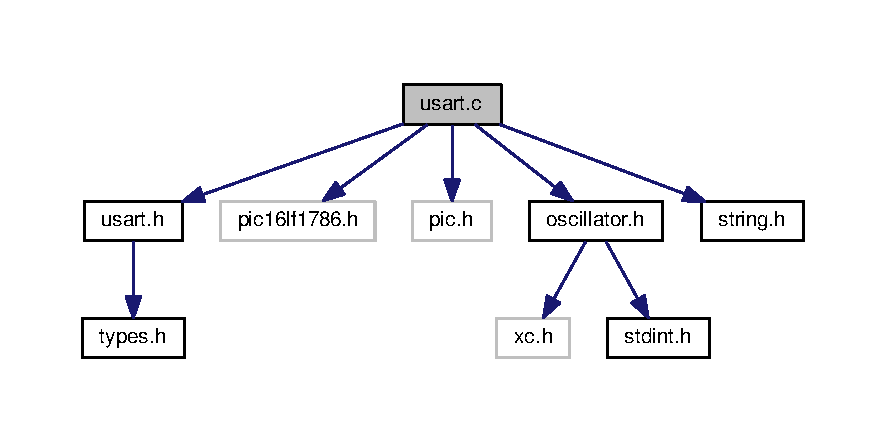
\includegraphics[width=350pt]{usart_8c__incl}
\end{center}
\end{figure}
\subsection*{Functions}
\begin{DoxyCompactItemize}
\item 
void \hyperlink{usart_8c_a8a68523fcfebe109df61258219ae9688}{usart\+\_\+start} (\hyperlink{usart_8h_a7ecd603d2579abbe714d58eb582821b8}{usart\+\_\+sync\+\_\+mode\+\_\+t} usart\+\_\+sync\+\_\+mode, \hyperlink{stdint_8h_a06896e8c53f721507066c079052171f8}{uint32\+\_\+t} baud\+\_\+rate)
\item 
void \hyperlink{usart_8c_aa813ecd58b112792997034433c01a391}{usart\+\_\+transmite\+\_\+set\+\_\+message} (char $\ast$message)
\item 
void \hyperlink{usart_8c_ace64d3f73f8d6f4deb50dcaab535be75}{usart\+\_\+transmite\+\_\+interrupt\+\_\+write\+\_\+message} (char $\ast$message, \hyperlink{types_8h_aa8204afb245708cfdad3878a09f1c83e}{callback\+\_\+isr\+\_\+t} usart\+\_\+callback\+\_\+transmit\+\_\+done)
\item 
void \hyperlink{usart_8c_a0f565c4ece40219cd8e0499edb19f600}{usart\+\_\+transmite\+\_\+interrupt\+\_\+isr} ()
\item 
void \hyperlink{usart_8c_a4464da3c14838dd54b5f9b0e5efc3e78}{usart\+\_\+transmite\+\_\+lock\+\_\+write\+\_\+byte} (\hyperlink{types_8h_a0c8186d9b9b7880309c27230bbb5e69d}{byte} data)
\item 
void \hyperlink{usart_8c_a3bdb4a2748bbd78e74f868415af429aa}{usart\+\_\+transmite\+\_\+lock\+\_\+write\+\_\+message} (char $\ast$message)
\item 
\hyperlink{types_8h_a0c8186d9b9b7880309c27230bbb5e69d}{byte} \hyperlink{usart_8c_a1ab1e3e47eb749bb56f1832b75c6790e}{usart\+\_\+receive\+\_\+lock\+\_\+read\+\_\+byte} ()
\item 
\hyperlink{stdint_8h_aba7bc1797add20fe3efdf37ced1182c5}{uint8\+\_\+t} \hyperlink{usart_8c_a9e13620a0dc60d72b792d501ff67c68d}{usart\+\_\+receive\+\_\+lock\+\_\+read\+\_\+message} (char $\ast$buffer, \hyperlink{stdint_8h_aba7bc1797add20fe3efdf37ced1182c5}{uint8\+\_\+t} size)
\item 
void \hyperlink{usart_8c_a56dc1cc4286dea0f752723577faf52cb}{usart\+\_\+receive\+\_\+interrupt\+\_\+read\+\_\+message} (\hyperlink{types_8h_aa8204afb245708cfdad3878a09f1c83e}{callback\+\_\+isr\+\_\+t} usart\+\_\+callback\+\_\+receive\+\_\+done)
\item 
void \hyperlink{usart_8c_a8016e6fb6f0a421fb1622403ccf7b16a}{usart\+\_\+receive\+\_\+interrupt\+\_\+isr} ()
\item 
char $\ast$ \hyperlink{usart_8c_ad731c697950fec7f25903623a1086fbf}{usart\+\_\+receive\+\_\+interrupt\+\_\+get\+\_\+message} ()
\end{DoxyCompactItemize}
\subsection*{Variables}
\begin{DoxyCompactItemize}
\item 
char \hyperlink{usart_8c_a89c9155c8f7952903c019986fdee1190}{\+\_\+tx\+\_\+buffer} \mbox{[}\hyperlink{usart_8h_a349dcc3059ac0d819919b4030de0ffe7}{T\+X\+\_\+\+B\+U\+F\+F\+E\+R\+\_\+\+M\+A\+X\+\_\+\+S\+I\+Z\+E}\mbox{]}
\item 
char $\ast$ \hyperlink{usart_8c_ac5b0349e3bd4facd6b5551f4815cb419}{\+\_\+tx\+\_\+buffer\+\_\+iterator} = \hyperlink{types_8h_a070d2ce7b6bb7e5c05602aa8c308d0c4}{N\+U\+L\+L}
\item 
\hyperlink{types_8h_aa8204afb245708cfdad3878a09f1c83e}{callback\+\_\+isr\+\_\+t} \hyperlink{usart_8c_aa3e7369accb462e77afd0ba3a7561130}{\+\_\+tx\+\_\+isr\+\_\+done\+\_\+callback} = \hyperlink{types_8h_a070d2ce7b6bb7e5c05602aa8c308d0c4}{N\+U\+L\+L}
\item 
char \hyperlink{usart_8c_a6754c15685eb75c32c1f20ccae374354}{\+\_\+rx\+\_\+buffer} \mbox{[}\hyperlink{usart_8h_a75e60ae3c6638b245ded9f9106f236e9}{R\+X\+\_\+\+B\+U\+F\+F\+E\+R\+\_\+\+M\+A\+X\+\_\+\+S\+I\+Z\+E}\mbox{]}
\item 
char $\ast$ \hyperlink{usart_8c_a4085826de4a75d06b8729276f71c6a37}{\+\_\+rx\+\_\+buffer\+\_\+iterator} = \hyperlink{types_8h_a070d2ce7b6bb7e5c05602aa8c308d0c4}{N\+U\+L\+L}
\item 
\hyperlink{types_8h_a0c8186d9b9b7880309c27230bbb5e69d}{byte} \hyperlink{usart_8c_a1f806581fc3c5c514048bb5abbb4b352}{\+\_\+rx\+\_\+buffer\+\_\+message\+\_\+size}
\item 
\hyperlink{types_8h_aa8204afb245708cfdad3878a09f1c83e}{callback\+\_\+isr\+\_\+t} \hyperlink{usart_8c_a6d9930601720515e24135b4dd1a052e7}{\+\_\+rx\+\_\+isr\+\_\+done\+\_\+callback} = \hyperlink{types_8h_a070d2ce7b6bb7e5c05602aa8c308d0c4}{N\+U\+L\+L}
\end{DoxyCompactItemize}


\subsection{Function Documentation}
\hypertarget{usart_8c_ad731c697950fec7f25903623a1086fbf}{\index{usart.\+c@{usart.\+c}!usart\+\_\+receive\+\_\+interrupt\+\_\+get\+\_\+message@{usart\+\_\+receive\+\_\+interrupt\+\_\+get\+\_\+message}}
\index{usart\+\_\+receive\+\_\+interrupt\+\_\+get\+\_\+message@{usart\+\_\+receive\+\_\+interrupt\+\_\+get\+\_\+message}!usart.\+c@{usart.\+c}}
\subsubsection[{usart\+\_\+receive\+\_\+interrupt\+\_\+get\+\_\+message}]{\setlength{\rightskip}{0pt plus 5cm}char$\ast$ usart\+\_\+receive\+\_\+interrupt\+\_\+get\+\_\+message (
\begin{DoxyParamCaption}
{}
\end{DoxyParamCaption}
)}}\label{usart_8c_ad731c697950fec7f25903623a1086fbf}
Recupera o ponteiro para a mensagem recebida ao final da interrup��o. \hypertarget{usart_8c_a8016e6fb6f0a421fb1622403ccf7b16a}{\index{usart.\+c@{usart.\+c}!usart\+\_\+receive\+\_\+interrupt\+\_\+isr@{usart\+\_\+receive\+\_\+interrupt\+\_\+isr}}
\index{usart\+\_\+receive\+\_\+interrupt\+\_\+isr@{usart\+\_\+receive\+\_\+interrupt\+\_\+isr}!usart.\+c@{usart.\+c}}
\subsubsection[{usart\+\_\+receive\+\_\+interrupt\+\_\+isr}]{\setlength{\rightskip}{0pt plus 5cm}void usart\+\_\+receive\+\_\+interrupt\+\_\+isr (
\begin{DoxyParamCaption}
{}
\end{DoxyParamCaption}
)}}\label{usart_8c_a8016e6fb6f0a421fb1622403ccf7b16a}
\begin{DoxyRemark}{Remarks}
N�o precisa chamar esta fun��o. Ela � chamada automaticamente pela fun��o tratadora de interrup��es. Fun��o que trata a interrup��o de recep��o de mensagem. 
\end{DoxyRemark}
\begin{DoxyRefDesc}{Todo}
\item[\hyperlink{todo__todo000004}{Todo}]Transformar em uma macro depois. \end{DoxyRefDesc}
\hypertarget{usart_8c_a56dc1cc4286dea0f752723577faf52cb}{\index{usart.\+c@{usart.\+c}!usart\+\_\+receive\+\_\+interrupt\+\_\+read\+\_\+message@{usart\+\_\+receive\+\_\+interrupt\+\_\+read\+\_\+message}}
\index{usart\+\_\+receive\+\_\+interrupt\+\_\+read\+\_\+message@{usart\+\_\+receive\+\_\+interrupt\+\_\+read\+\_\+message}!usart.\+c@{usart.\+c}}
\subsubsection[{usart\+\_\+receive\+\_\+interrupt\+\_\+read\+\_\+message}]{\setlength{\rightskip}{0pt plus 5cm}void usart\+\_\+receive\+\_\+interrupt\+\_\+read\+\_\+message (
\begin{DoxyParamCaption}
\item[{{\bf callback\+\_\+isr\+\_\+t}}]{usart\+\_\+callback\+\_\+receive\+\_\+done}
\end{DoxyParamCaption}
)}}\label{usart_8c_a56dc1cc4286dea0f752723577faf52cb}
Recebe uma string inteira, utilizando interrup��es. A string deve terminar em ''. 
\begin{DoxyParams}{Parameters}
{\em usart\+\_\+callback\+\_\+receive\+\_\+done} & fun��o que ser� chamada quando a mensagem for totalmente recebida. \\
\hline
\end{DoxyParams}
\hypertarget{usart_8c_a1ab1e3e47eb749bb56f1832b75c6790e}{\index{usart.\+c@{usart.\+c}!usart\+\_\+receive\+\_\+lock\+\_\+read\+\_\+byte@{usart\+\_\+receive\+\_\+lock\+\_\+read\+\_\+byte}}
\index{usart\+\_\+receive\+\_\+lock\+\_\+read\+\_\+byte@{usart\+\_\+receive\+\_\+lock\+\_\+read\+\_\+byte}!usart.\+c@{usart.\+c}}
\subsubsection[{usart\+\_\+receive\+\_\+lock\+\_\+read\+\_\+byte}]{\setlength{\rightskip}{0pt plus 5cm}{\bf byte} usart\+\_\+receive\+\_\+lock\+\_\+read\+\_\+byte (
\begin{DoxyParamCaption}
{}
\end{DoxyParamCaption}
)}}\label{usart_8c_a1ab1e3e47eb749bb56f1832b75c6790e}
Recebe um byte (mas trava a tarefa). \begin{DoxyReturn}{Returns}
O valor recebido do R\+X. 
\end{DoxyReturn}
\hypertarget{usart_8c_a9e13620a0dc60d72b792d501ff67c68d}{\index{usart.\+c@{usart.\+c}!usart\+\_\+receive\+\_\+lock\+\_\+read\+\_\+message@{usart\+\_\+receive\+\_\+lock\+\_\+read\+\_\+message}}
\index{usart\+\_\+receive\+\_\+lock\+\_\+read\+\_\+message@{usart\+\_\+receive\+\_\+lock\+\_\+read\+\_\+message}!usart.\+c@{usart.\+c}}
\subsubsection[{usart\+\_\+receive\+\_\+lock\+\_\+read\+\_\+message}]{\setlength{\rightskip}{0pt plus 5cm}{\bf uint8\+\_\+t} usart\+\_\+receive\+\_\+lock\+\_\+read\+\_\+message (
\begin{DoxyParamCaption}
\item[{char $\ast$}]{buffer, }
\item[{{\bf uint8\+\_\+t}}]{size}
\end{DoxyParamCaption}
)}}\label{usart_8c_a9e13620a0dc60d72b792d501ff67c68d}
Recebe uma string inteira (mas trava a tarefa). A string deve terminar em ''. 
\begin{DoxyParams}{Parameters}
{\em buffer} & O buffer onde a mensagem ser� salva. \\
\hline
{\em size} & O tamanho do buffer. \\
\hline
\end{DoxyParams}
\begin{DoxyReturn}{Returns}
A quantidade de caracteres recebida. 
\end{DoxyReturn}
\hypertarget{usart_8c_a8a68523fcfebe109df61258219ae9688}{\index{usart.\+c@{usart.\+c}!usart\+\_\+start@{usart\+\_\+start}}
\index{usart\+\_\+start@{usart\+\_\+start}!usart.\+c@{usart.\+c}}
\subsubsection[{usart\+\_\+start}]{\setlength{\rightskip}{0pt plus 5cm}void usart\+\_\+start (
\begin{DoxyParamCaption}
\item[{{\bf usart\+\_\+sync\+\_\+mode\+\_\+t}}]{usart\+\_\+sync\+\_\+mode, }
\item[{{\bf uint32\+\_\+t}}]{baud\+\_\+rate}
\end{DoxyParamCaption}
)}}\label{usart_8c_a8a68523fcfebe109df61258219ae9688}
Inicia a comunica��o por E\+U\+S\+A\+R\+T.


\begin{DoxyParams}{Parameters}
{\em usart\+\_\+sync\+\_\+mode} & Modo de sincroniza��o desejado. Por hora, s� tem Assincrono. \\
\hline
{\em baud\+\_\+rate} & Velocidade da transferencia. Existem constantes definidas com os valores mais comuns. \\
\hline
\end{DoxyParams}
\begin{DoxyRefDesc}{Todo}
\item[\hyperlink{todo__todo000002}{Todo}]Implementar modo sincrono! \end{DoxyRefDesc}
\hypertarget{usart_8c_a0f565c4ece40219cd8e0499edb19f600}{\index{usart.\+c@{usart.\+c}!usart\+\_\+transmite\+\_\+interrupt\+\_\+isr@{usart\+\_\+transmite\+\_\+interrupt\+\_\+isr}}
\index{usart\+\_\+transmite\+\_\+interrupt\+\_\+isr@{usart\+\_\+transmite\+\_\+interrupt\+\_\+isr}!usart.\+c@{usart.\+c}}
\subsubsection[{usart\+\_\+transmite\+\_\+interrupt\+\_\+isr}]{\setlength{\rightskip}{0pt plus 5cm}void usart\+\_\+transmite\+\_\+interrupt\+\_\+isr (
\begin{DoxyParamCaption}
{}
\end{DoxyParamCaption}
)}}\label{usart_8c_a0f565c4ece40219cd8e0499edb19f600}
\begin{DoxyRemark}{Remarks}
N�o precisa chamar esta fun��o. Ela � chamada automaticamente pela fun��o tratadora de interrup��es. Fun��o que trata a interrup��o de envio de mensagem. 
\end{DoxyRemark}
\begin{DoxyRefDesc}{Todo}
\item[\hyperlink{todo__todo000003}{Todo}]Transformar em uma macro depois. \end{DoxyRefDesc}
\hypertarget{usart_8c_ace64d3f73f8d6f4deb50dcaab535be75}{\index{usart.\+c@{usart.\+c}!usart\+\_\+transmite\+\_\+interrupt\+\_\+write\+\_\+message@{usart\+\_\+transmite\+\_\+interrupt\+\_\+write\+\_\+message}}
\index{usart\+\_\+transmite\+\_\+interrupt\+\_\+write\+\_\+message@{usart\+\_\+transmite\+\_\+interrupt\+\_\+write\+\_\+message}!usart.\+c@{usart.\+c}}
\subsubsection[{usart\+\_\+transmite\+\_\+interrupt\+\_\+write\+\_\+message}]{\setlength{\rightskip}{0pt plus 5cm}void usart\+\_\+transmite\+\_\+interrupt\+\_\+write\+\_\+message (
\begin{DoxyParamCaption}
\item[{char $\ast$}]{message, }
\item[{{\bf callback\+\_\+isr\+\_\+t}}]{usart\+\_\+callback\+\_\+transmit\+\_\+done}
\end{DoxyParamCaption}
)}}\label{usart_8c_ace64d3f73f8d6f4deb50dcaab535be75}
Transmite uma mensagem, utilizando interrup��es. 
\begin{DoxyParams}{Parameters}
{\em message} & String que ser� enviada. \\
\hline
{\em usart\+\_\+callback\+\_\+transmit\+\_\+done} & Fun��o que ser� chamada ap�s o ultimo byte ser transmitido. \\
\hline
\end{DoxyParams}
\hypertarget{usart_8c_a4464da3c14838dd54b5f9b0e5efc3e78}{\index{usart.\+c@{usart.\+c}!usart\+\_\+transmite\+\_\+lock\+\_\+write\+\_\+byte@{usart\+\_\+transmite\+\_\+lock\+\_\+write\+\_\+byte}}
\index{usart\+\_\+transmite\+\_\+lock\+\_\+write\+\_\+byte@{usart\+\_\+transmite\+\_\+lock\+\_\+write\+\_\+byte}!usart.\+c@{usart.\+c}}
\subsubsection[{usart\+\_\+transmite\+\_\+lock\+\_\+write\+\_\+byte}]{\setlength{\rightskip}{0pt plus 5cm}void usart\+\_\+transmite\+\_\+lock\+\_\+write\+\_\+byte (
\begin{DoxyParamCaption}
\item[{{\bf byte}}]{data}
\end{DoxyParamCaption}
)}}\label{usart_8c_a4464da3c14838dd54b5f9b0e5efc3e78}
\begin{DoxyRemark}{Remarks}
Fun��o privada (N�o acessivel de fora -\/ n�o � pra cagar nela).
\end{DoxyRemark}
Transmite um byte (mas trava a tarefa).


\begin{DoxyParams}{Parameters}
{\em data} & Byte que ser� transmitido. \\
\hline
\end{DoxyParams}
\hypertarget{usart_8c_a3bdb4a2748bbd78e74f868415af429aa}{\index{usart.\+c@{usart.\+c}!usart\+\_\+transmite\+\_\+lock\+\_\+write\+\_\+message@{usart\+\_\+transmite\+\_\+lock\+\_\+write\+\_\+message}}
\index{usart\+\_\+transmite\+\_\+lock\+\_\+write\+\_\+message@{usart\+\_\+transmite\+\_\+lock\+\_\+write\+\_\+message}!usart.\+c@{usart.\+c}}
\subsubsection[{usart\+\_\+transmite\+\_\+lock\+\_\+write\+\_\+message}]{\setlength{\rightskip}{0pt plus 5cm}void usart\+\_\+transmite\+\_\+lock\+\_\+write\+\_\+message (
\begin{DoxyParamCaption}
\item[{char $\ast$}]{message}
\end{DoxyParamCaption}
)}}\label{usart_8c_a3bdb4a2748bbd78e74f868415af429aa}
Transmite uma string (mas trava a tarefa). 
\begin{DoxyParams}{Parameters}
{\em message} & String que ser� transmitida. \\
\hline
\end{DoxyParams}
\hypertarget{usart_8c_aa813ecd58b112792997034433c01a391}{\index{usart.\+c@{usart.\+c}!usart\+\_\+transmite\+\_\+set\+\_\+message@{usart\+\_\+transmite\+\_\+set\+\_\+message}}
\index{usart\+\_\+transmite\+\_\+set\+\_\+message@{usart\+\_\+transmite\+\_\+set\+\_\+message}!usart.\+c@{usart.\+c}}
\subsubsection[{usart\+\_\+transmite\+\_\+set\+\_\+message}]{\setlength{\rightskip}{0pt plus 5cm}void usart\+\_\+transmite\+\_\+set\+\_\+message (
\begin{DoxyParamCaption}
\item[{char $\ast$}]{message}
\end{DoxyParamCaption}
)}}\label{usart_8c_aa813ecd58b112792997034433c01a391}
\begin{DoxyRemark}{Remarks}
Fun��o privada (N�o acessivel de fora -\/ n�o � pra cagar nela).
\end{DoxyRemark}
Fun��o que copia a mensagem para um buffer interno E cria um iterador (ponteiro) para percorre ela. 

\subsection{Variable Documentation}
\hypertarget{usart_8c_a6754c15685eb75c32c1f20ccae374354}{\index{usart.\+c@{usart.\+c}!\+\_\+rx\+\_\+buffer@{\+\_\+rx\+\_\+buffer}}
\index{\+\_\+rx\+\_\+buffer@{\+\_\+rx\+\_\+buffer}!usart.\+c@{usart.\+c}}
\subsubsection[{\+\_\+rx\+\_\+buffer}]{\setlength{\rightskip}{0pt plus 5cm}char \+\_\+rx\+\_\+buffer\mbox{[}{\bf R\+X\+\_\+\+B\+U\+F\+F\+E\+R\+\_\+\+M\+A\+X\+\_\+\+S\+I\+Z\+E}\mbox{]}}}\label{usart_8c_a6754c15685eb75c32c1f20ccae374354}
Buffer para recebimento de mensagens \hypertarget{usart_8c_a4085826de4a75d06b8729276f71c6a37}{\index{usart.\+c@{usart.\+c}!\+\_\+rx\+\_\+buffer\+\_\+iterator@{\+\_\+rx\+\_\+buffer\+\_\+iterator}}
\index{\+\_\+rx\+\_\+buffer\+\_\+iterator@{\+\_\+rx\+\_\+buffer\+\_\+iterator}!usart.\+c@{usart.\+c}}
\subsubsection[{\+\_\+rx\+\_\+buffer\+\_\+iterator}]{\setlength{\rightskip}{0pt plus 5cm}char$\ast$ \+\_\+rx\+\_\+buffer\+\_\+iterator = {\bf N\+U\+L\+L}}}\label{usart_8c_a4085826de4a75d06b8729276f71c6a37}
Iterador do buffer de recebimento \hypertarget{usart_8c_a1f806581fc3c5c514048bb5abbb4b352}{\index{usart.\+c@{usart.\+c}!\+\_\+rx\+\_\+buffer\+\_\+message\+\_\+size@{\+\_\+rx\+\_\+buffer\+\_\+message\+\_\+size}}
\index{\+\_\+rx\+\_\+buffer\+\_\+message\+\_\+size@{\+\_\+rx\+\_\+buffer\+\_\+message\+\_\+size}!usart.\+c@{usart.\+c}}
\subsubsection[{\+\_\+rx\+\_\+buffer\+\_\+message\+\_\+size}]{\setlength{\rightskip}{0pt plus 5cm}{\bf byte} \+\_\+rx\+\_\+buffer\+\_\+message\+\_\+size}}\label{usart_8c_a1f806581fc3c5c514048bb5abbb4b352}
Tamanho da mensagem recebida pelo buffer \hypertarget{usart_8c_a6d9930601720515e24135b4dd1a052e7}{\index{usart.\+c@{usart.\+c}!\+\_\+rx\+\_\+isr\+\_\+done\+\_\+callback@{\+\_\+rx\+\_\+isr\+\_\+done\+\_\+callback}}
\index{\+\_\+rx\+\_\+isr\+\_\+done\+\_\+callback@{\+\_\+rx\+\_\+isr\+\_\+done\+\_\+callback}!usart.\+c@{usart.\+c}}
\subsubsection[{\+\_\+rx\+\_\+isr\+\_\+done\+\_\+callback}]{\setlength{\rightskip}{0pt plus 5cm}{\bf callback\+\_\+isr\+\_\+t} \+\_\+rx\+\_\+isr\+\_\+done\+\_\+callback = {\bf N\+U\+L\+L}}}\label{usart_8c_a6d9930601720515e24135b4dd1a052e7}
Fun��o disparda quando uma mensagem for totalmente recebida (terminada em 'r') \hypertarget{usart_8c_a89c9155c8f7952903c019986fdee1190}{\index{usart.\+c@{usart.\+c}!\+\_\+tx\+\_\+buffer@{\+\_\+tx\+\_\+buffer}}
\index{\+\_\+tx\+\_\+buffer@{\+\_\+tx\+\_\+buffer}!usart.\+c@{usart.\+c}}
\subsubsection[{\+\_\+tx\+\_\+buffer}]{\setlength{\rightskip}{0pt plus 5cm}char \+\_\+tx\+\_\+buffer\mbox{[}{\bf T\+X\+\_\+\+B\+U\+F\+F\+E\+R\+\_\+\+M\+A\+X\+\_\+\+S\+I\+Z\+E}\mbox{]}}}\label{usart_8c_a89c9155c8f7952903c019986fdee1190}
Buffer para envio de mensagens \hypertarget{usart_8c_ac5b0349e3bd4facd6b5551f4815cb419}{\index{usart.\+c@{usart.\+c}!\+\_\+tx\+\_\+buffer\+\_\+iterator@{\+\_\+tx\+\_\+buffer\+\_\+iterator}}
\index{\+\_\+tx\+\_\+buffer\+\_\+iterator@{\+\_\+tx\+\_\+buffer\+\_\+iterator}!usart.\+c@{usart.\+c}}
\subsubsection[{\+\_\+tx\+\_\+buffer\+\_\+iterator}]{\setlength{\rightskip}{0pt plus 5cm}char$\ast$ \+\_\+tx\+\_\+buffer\+\_\+iterator = {\bf N\+U\+L\+L}}}\label{usart_8c_ac5b0349e3bd4facd6b5551f4815cb419}
Iterador do buffer de envio \hypertarget{usart_8c_aa3e7369accb462e77afd0ba3a7561130}{\index{usart.\+c@{usart.\+c}!\+\_\+tx\+\_\+isr\+\_\+done\+\_\+callback@{\+\_\+tx\+\_\+isr\+\_\+done\+\_\+callback}}
\index{\+\_\+tx\+\_\+isr\+\_\+done\+\_\+callback@{\+\_\+tx\+\_\+isr\+\_\+done\+\_\+callback}!usart.\+c@{usart.\+c}}
\subsubsection[{\+\_\+tx\+\_\+isr\+\_\+done\+\_\+callback}]{\setlength{\rightskip}{0pt plus 5cm}{\bf callback\+\_\+isr\+\_\+t} \+\_\+tx\+\_\+isr\+\_\+done\+\_\+callback = {\bf N\+U\+L\+L}}}\label{usart_8c_aa3e7369accb462e77afd0ba3a7561130}
Fun��o disparda quando a mensagem for totalmente enviada no modo por interrup��o 
\hypertarget{usart_8h}{\section{usart.\+h File Reference}
\label{usart_8h}\index{usart.\+h@{usart.\+h}}
}
{\ttfamily \#include \char`\"{}types.\+h\char`\"{}}\\*
Include dependency graph for usart.\+h\+:\nopagebreak
\begin{figure}[H]
\begin{center}
\leavevmode
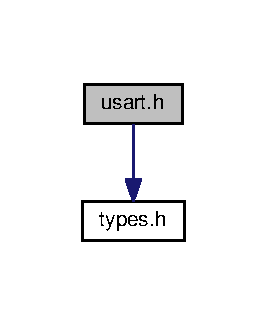
\includegraphics[width=128pt]{usart_8h__incl}
\end{center}
\end{figure}
This graph shows which files directly or indirectly include this file\+:\nopagebreak
\begin{figure}[H]
\begin{center}
\leavevmode
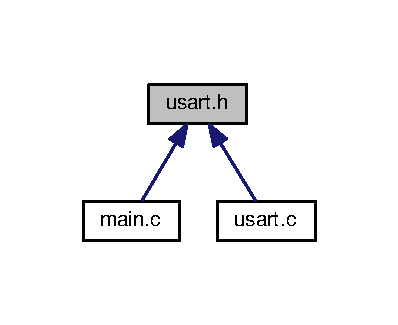
\includegraphics[width=191pt]{usart_8h__dep__incl}
\end{center}
\end{figure}
\subsection*{Macros}
\begin{DoxyCompactItemize}
\item 
\#define \hyperlink{usart_8h_a349dcc3059ac0d819919b4030de0ffe7}{T\+X\+\_\+\+B\+U\+F\+F\+E\+R\+\_\+\+M\+A\+X\+\_\+\+S\+I\+Z\+E}~61
\item 
\#define \hyperlink{usart_8h_a75e60ae3c6638b245ded9f9106f236e9}{R\+X\+\_\+\+B\+U\+F\+F\+E\+R\+\_\+\+M\+A\+X\+\_\+\+S\+I\+Z\+E}~61
\end{DoxyCompactItemize}
\subsection*{Enumerations}
\begin{DoxyCompactItemize}
\item 
enum \hyperlink{usart_8h_a7ecd603d2579abbe714d58eb582821b8}{usart\+\_\+sync\+\_\+mode\+\_\+t} \{ \hyperlink{usart_8h_a7ecd603d2579abbe714d58eb582821b8a1a8ad112420639e0d8b7b5d03fec821b}{U\+S\+A\+R\+T\+\_\+\+S\+Y\+N\+C\+\_\+\+M\+O\+D\+E\+\_\+\+A\+S\+Y\+N\+C\+H\+R\+O\+N\+O\+U\+S} = L\+O\+W, 
\hyperlink{usart_8h_a7ecd603d2579abbe714d58eb582821b8a34d87ffc3dd86d3b66b0dd395a2dd921}{U\+S\+A\+R\+T\+\_\+\+S\+Y\+N\+C\+\_\+\+M\+O\+D\+E\+\_\+\+S\+Y\+N\+C\+H\+R\+O\+N\+O\+U\+S} = H\+I\+G\+H
 \}
\item 
enum \hyperlink{usart_8h_ac9a70b65ef766451441f01b9481796ce}{usart\+\_\+9bit\+\_\+mode\+\_\+t} \{ \hyperlink{usart_8h_ac9a70b65ef766451441f01b9481796cea32cb2a138110deff6810efd4d203459a}{U\+S\+A\+R\+T\+\_\+9\+B\+I\+T\+\_\+\+M\+O\+D\+E\+\_\+\+N\+O\+T\+\_\+\+I\+M\+P\+L\+E\+M\+E\+N\+T\+E\+D} = L\+O\+W
 \}
\end{DoxyCompactItemize}
\subsection*{Functions}
\begin{DoxyCompactItemize}
\item 
void \hyperlink{usart_8h_a8a68523fcfebe109df61258219ae9688}{usart\+\_\+start} (\hyperlink{usart_8h_a7ecd603d2579abbe714d58eb582821b8}{usart\+\_\+sync\+\_\+mode\+\_\+t} usart\+\_\+sync\+\_\+mode, \hyperlink{stdint_8h_a06896e8c53f721507066c079052171f8}{uint32\+\_\+t} baud\+\_\+rate)
\item 
void \hyperlink{usart_8h_ace64d3f73f8d6f4deb50dcaab535be75}{usart\+\_\+transmite\+\_\+interrupt\+\_\+write\+\_\+message} (char $\ast$message, \hyperlink{types_8h_aa8204afb245708cfdad3878a09f1c83e}{callback\+\_\+isr\+\_\+t} usart\+\_\+callback\+\_\+transmit\+\_\+done)
\item 
void \hyperlink{usart_8h_a0f565c4ece40219cd8e0499edb19f600}{usart\+\_\+transmite\+\_\+interrupt\+\_\+isr} ()
\item 
void \hyperlink{usart_8h_a4464da3c14838dd54b5f9b0e5efc3e78}{usart\+\_\+transmite\+\_\+lock\+\_\+write\+\_\+byte} (\hyperlink{types_8h_a0c8186d9b9b7880309c27230bbb5e69d}{byte} data)
\item 
void \hyperlink{usart_8h_a3bdb4a2748bbd78e74f868415af429aa}{usart\+\_\+transmite\+\_\+lock\+\_\+write\+\_\+message} (char $\ast$message)
\item 
\hyperlink{types_8h_a0c8186d9b9b7880309c27230bbb5e69d}{byte} \hyperlink{usart_8h_a1ab1e3e47eb749bb56f1832b75c6790e}{usart\+\_\+receive\+\_\+lock\+\_\+read\+\_\+byte} ()
\item 
\hyperlink{stdint_8h_aba7bc1797add20fe3efdf37ced1182c5}{uint8\+\_\+t} \hyperlink{usart_8h_a9e13620a0dc60d72b792d501ff67c68d}{usart\+\_\+receive\+\_\+lock\+\_\+read\+\_\+message} (char $\ast$buffer, \hyperlink{stdint_8h_aba7bc1797add20fe3efdf37ced1182c5}{uint8\+\_\+t} size)
\item 
void \hyperlink{usart_8h_a56dc1cc4286dea0f752723577faf52cb}{usart\+\_\+receive\+\_\+interrupt\+\_\+read\+\_\+message} (\hyperlink{types_8h_aa8204afb245708cfdad3878a09f1c83e}{callback\+\_\+isr\+\_\+t} usart\+\_\+callback\+\_\+receive\+\_\+done)
\item 
void \hyperlink{usart_8h_a8016e6fb6f0a421fb1622403ccf7b16a}{usart\+\_\+receive\+\_\+interrupt\+\_\+isr} ()
\item 
char $\ast$ \hyperlink{usart_8h_ad731c697950fec7f25903623a1086fbf}{usart\+\_\+receive\+\_\+interrupt\+\_\+get\+\_\+message} ()
\end{DoxyCompactItemize}
\subsection*{Variables}
\begin{DoxyCompactItemize}
\item 
const \hyperlink{stdint_8h_a06896e8c53f721507066c079052171f8}{uint32\+\_\+t} \hyperlink{usart_8h_a71b7a36a4e5cff9229a2d49a655009bc}{U\+S\+A\+R\+T\+\_\+\+B\+A\+U\+D\+\_\+\+R\+A\+T\+E\+\_\+300} = 300ul
\item 
const \hyperlink{stdint_8h_a06896e8c53f721507066c079052171f8}{uint32\+\_\+t} \hyperlink{usart_8h_a2d4acc87bd9c689e52d0ea74d0e376bd}{U\+S\+A\+R\+T\+\_\+\+B\+A\+U\+D\+\_\+\+R\+A\+T\+E\+\_\+484} = 484ul
\item 
const \hyperlink{stdint_8h_a06896e8c53f721507066c079052171f8}{uint32\+\_\+t} \hyperlink{usart_8h_a79e796d8f0eca10a8700c39a271f766e}{U\+S\+A\+R\+T\+\_\+\+B\+A\+U\+D\+\_\+\+R\+A\+T\+E\+\_\+1200} = 1200ul
\item 
const \hyperlink{stdint_8h_a06896e8c53f721507066c079052171f8}{uint32\+\_\+t} \hyperlink{usart_8h_aab78c07ac38da93743ccd5a93030bffa}{U\+S\+A\+R\+T\+\_\+\+B\+A\+U\+D\+\_\+\+R\+A\+T\+E\+\_\+2400} = 2400ul
\item 
const \hyperlink{stdint_8h_a06896e8c53f721507066c079052171f8}{uint32\+\_\+t} \hyperlink{usart_8h_ac83aa1b365f9c085b2762980926ee594}{U\+S\+A\+R\+T\+\_\+\+B\+A\+U\+D\+\_\+\+R\+A\+T\+E\+\_\+9600} = 9600ul
\item 
const \hyperlink{stdint_8h_a06896e8c53f721507066c079052171f8}{uint32\+\_\+t} \hyperlink{usart_8h_aba561abfb08dede0c4e54a88f40c8841}{U\+S\+A\+R\+T\+\_\+\+B\+A\+U\+D\+\_\+\+R\+A\+T\+E\+\_\+10417} = 10417ul
\item 
const \hyperlink{stdint_8h_a06896e8c53f721507066c079052171f8}{uint32\+\_\+t} \hyperlink{usart_8h_a748949f9c355484b8715f2510125c0a8}{U\+S\+A\+R\+T\+\_\+\+B\+A\+U\+D\+\_\+\+R\+A\+T\+E\+\_\+19200} = 19200ul
\item 
const \hyperlink{stdint_8h_a06896e8c53f721507066c079052171f8}{uint32\+\_\+t} \hyperlink{usart_8h_a090428649014dc41404227c791a8d357}{U\+S\+A\+R\+T\+\_\+\+B\+A\+U\+D\+\_\+\+R\+A\+T\+E\+\_\+57600} = 57600ul
\item 
const \hyperlink{stdint_8h_a06896e8c53f721507066c079052171f8}{uint32\+\_\+t} \hyperlink{usart_8h_a47d90ebe1d09a984ab87e2013ad97cf8}{U\+S\+A\+R\+T\+\_\+\+B\+A\+U\+D\+\_\+\+R\+A\+T\+E\+\_\+115200} = 115200ul
\end{DoxyCompactItemize}


\subsection{Macro Definition Documentation}
\hypertarget{usart_8h_a75e60ae3c6638b245ded9f9106f236e9}{\index{usart.\+h@{usart.\+h}!R\+X\+\_\+\+B\+U\+F\+F\+E\+R\+\_\+\+M\+A\+X\+\_\+\+S\+I\+Z\+E@{R\+X\+\_\+\+B\+U\+F\+F\+E\+R\+\_\+\+M\+A\+X\+\_\+\+S\+I\+Z\+E}}
\index{R\+X\+\_\+\+B\+U\+F\+F\+E\+R\+\_\+\+M\+A\+X\+\_\+\+S\+I\+Z\+E@{R\+X\+\_\+\+B\+U\+F\+F\+E\+R\+\_\+\+M\+A\+X\+\_\+\+S\+I\+Z\+E}!usart.\+h@{usart.\+h}}
\subsubsection[{R\+X\+\_\+\+B\+U\+F\+F\+E\+R\+\_\+\+M\+A\+X\+\_\+\+S\+I\+Z\+E}]{\setlength{\rightskip}{0pt plus 5cm}\#define R\+X\+\_\+\+B\+U\+F\+F\+E\+R\+\_\+\+M\+A\+X\+\_\+\+S\+I\+Z\+E~61}}\label{usart_8h_a75e60ae3c6638b245ded9f9106f236e9}
\hypertarget{usart_8h_a349dcc3059ac0d819919b4030de0ffe7}{\index{usart.\+h@{usart.\+h}!T\+X\+\_\+\+B\+U\+F\+F\+E\+R\+\_\+\+M\+A\+X\+\_\+\+S\+I\+Z\+E@{T\+X\+\_\+\+B\+U\+F\+F\+E\+R\+\_\+\+M\+A\+X\+\_\+\+S\+I\+Z\+E}}
\index{T\+X\+\_\+\+B\+U\+F\+F\+E\+R\+\_\+\+M\+A\+X\+\_\+\+S\+I\+Z\+E@{T\+X\+\_\+\+B\+U\+F\+F\+E\+R\+\_\+\+M\+A\+X\+\_\+\+S\+I\+Z\+E}!usart.\+h@{usart.\+h}}
\subsubsection[{T\+X\+\_\+\+B\+U\+F\+F\+E\+R\+\_\+\+M\+A\+X\+\_\+\+S\+I\+Z\+E}]{\setlength{\rightskip}{0pt plus 5cm}\#define T\+X\+\_\+\+B\+U\+F\+F\+E\+R\+\_\+\+M\+A\+X\+\_\+\+S\+I\+Z\+E~61}}\label{usart_8h_a349dcc3059ac0d819919b4030de0ffe7}


\subsection{Enumeration Type Documentation}
\hypertarget{usart_8h_ac9a70b65ef766451441f01b9481796ce}{\index{usart.\+h@{usart.\+h}!usart\+\_\+9bit\+\_\+mode\+\_\+t@{usart\+\_\+9bit\+\_\+mode\+\_\+t}}
\index{usart\+\_\+9bit\+\_\+mode\+\_\+t@{usart\+\_\+9bit\+\_\+mode\+\_\+t}!usart.\+h@{usart.\+h}}
\subsubsection[{usart\+\_\+9bit\+\_\+mode\+\_\+t}]{\setlength{\rightskip}{0pt plus 5cm}enum {\bf usart\+\_\+9bit\+\_\+mode\+\_\+t}}}\label{usart_8h_ac9a70b65ef766451441f01b9481796ce}
\begin{Desc}
\item[Enumerator]\par
\begin{description}
\index{U\+S\+A\+R\+T\+\_\+9\+B\+I\+T\+\_\+\+M\+O\+D\+E\+\_\+\+N\+O\+T\+\_\+\+I\+M\+P\+L\+E\+M\+E\+N\+T\+E\+D@{U\+S\+A\+R\+T\+\_\+9\+B\+I\+T\+\_\+\+M\+O\+D\+E\+\_\+\+N\+O\+T\+\_\+\+I\+M\+P\+L\+E\+M\+E\+N\+T\+E\+D}!usart.\+h@{usart.\+h}}\index{usart.\+h@{usart.\+h}!U\+S\+A\+R\+T\+\_\+9\+B\+I\+T\+\_\+\+M\+O\+D\+E\+\_\+\+N\+O\+T\+\_\+\+I\+M\+P\+L\+E\+M\+E\+N\+T\+E\+D@{U\+S\+A\+R\+T\+\_\+9\+B\+I\+T\+\_\+\+M\+O\+D\+E\+\_\+\+N\+O\+T\+\_\+\+I\+M\+P\+L\+E\+M\+E\+N\+T\+E\+D}}\item[{\em 
\hypertarget{usart_8h_ac9a70b65ef766451441f01b9481796cea32cb2a138110deff6810efd4d203459a}{U\+S\+A\+R\+T\+\_\+9\+B\+I\+T\+\_\+\+M\+O\+D\+E\+\_\+\+N\+O\+T\+\_\+\+I\+M\+P\+L\+E\+M\+E\+N\+T\+E\+D}\label{usart_8h_ac9a70b65ef766451441f01b9481796cea32cb2a138110deff6810efd4d203459a}
}]\end{description}
\end{Desc}
\hypertarget{usart_8h_a7ecd603d2579abbe714d58eb582821b8}{\index{usart.\+h@{usart.\+h}!usart\+\_\+sync\+\_\+mode\+\_\+t@{usart\+\_\+sync\+\_\+mode\+\_\+t}}
\index{usart\+\_\+sync\+\_\+mode\+\_\+t@{usart\+\_\+sync\+\_\+mode\+\_\+t}!usart.\+h@{usart.\+h}}
\subsubsection[{usart\+\_\+sync\+\_\+mode\+\_\+t}]{\setlength{\rightskip}{0pt plus 5cm}enum {\bf usart\+\_\+sync\+\_\+mode\+\_\+t}}}\label{usart_8h_a7ecd603d2579abbe714d58eb582821b8}
\begin{Desc}
\item[Enumerator]\par
\begin{description}
\index{U\+S\+A\+R\+T\+\_\+\+S\+Y\+N\+C\+\_\+\+M\+O\+D\+E\+\_\+\+A\+S\+Y\+N\+C\+H\+R\+O\+N\+O\+U\+S@{U\+S\+A\+R\+T\+\_\+\+S\+Y\+N\+C\+\_\+\+M\+O\+D\+E\+\_\+\+A\+S\+Y\+N\+C\+H\+R\+O\+N\+O\+U\+S}!usart.\+h@{usart.\+h}}\index{usart.\+h@{usart.\+h}!U\+S\+A\+R\+T\+\_\+\+S\+Y\+N\+C\+\_\+\+M\+O\+D\+E\+\_\+\+A\+S\+Y\+N\+C\+H\+R\+O\+N\+O\+U\+S@{U\+S\+A\+R\+T\+\_\+\+S\+Y\+N\+C\+\_\+\+M\+O\+D\+E\+\_\+\+A\+S\+Y\+N\+C\+H\+R\+O\+N\+O\+U\+S}}\item[{\em 
\hypertarget{usart_8h_a7ecd603d2579abbe714d58eb582821b8a1a8ad112420639e0d8b7b5d03fec821b}{U\+S\+A\+R\+T\+\_\+\+S\+Y\+N\+C\+\_\+\+M\+O\+D\+E\+\_\+\+A\+S\+Y\+N\+C\+H\+R\+O\+N\+O\+U\+S}\label{usart_8h_a7ecd603d2579abbe714d58eb582821b8a1a8ad112420639e0d8b7b5d03fec821b}
}]\index{U\+S\+A\+R\+T\+\_\+\+S\+Y\+N\+C\+\_\+\+M\+O\+D\+E\+\_\+\+S\+Y\+N\+C\+H\+R\+O\+N\+O\+U\+S@{U\+S\+A\+R\+T\+\_\+\+S\+Y\+N\+C\+\_\+\+M\+O\+D\+E\+\_\+\+S\+Y\+N\+C\+H\+R\+O\+N\+O\+U\+S}!usart.\+h@{usart.\+h}}\index{usart.\+h@{usart.\+h}!U\+S\+A\+R\+T\+\_\+\+S\+Y\+N\+C\+\_\+\+M\+O\+D\+E\+\_\+\+S\+Y\+N\+C\+H\+R\+O\+N\+O\+U\+S@{U\+S\+A\+R\+T\+\_\+\+S\+Y\+N\+C\+\_\+\+M\+O\+D\+E\+\_\+\+S\+Y\+N\+C\+H\+R\+O\+N\+O\+U\+S}}\item[{\em 
\hypertarget{usart_8h_a7ecd603d2579abbe714d58eb582821b8a34d87ffc3dd86d3b66b0dd395a2dd921}{U\+S\+A\+R\+T\+\_\+\+S\+Y\+N\+C\+\_\+\+M\+O\+D\+E\+\_\+\+S\+Y\+N\+C\+H\+R\+O\+N\+O\+U\+S}\label{usart_8h_a7ecd603d2579abbe714d58eb582821b8a34d87ffc3dd86d3b66b0dd395a2dd921}
}]\end{description}
\end{Desc}


\subsection{Function Documentation}
\hypertarget{usart_8h_ad731c697950fec7f25903623a1086fbf}{\index{usart.\+h@{usart.\+h}!usart\+\_\+receive\+\_\+interrupt\+\_\+get\+\_\+message@{usart\+\_\+receive\+\_\+interrupt\+\_\+get\+\_\+message}}
\index{usart\+\_\+receive\+\_\+interrupt\+\_\+get\+\_\+message@{usart\+\_\+receive\+\_\+interrupt\+\_\+get\+\_\+message}!usart.\+h@{usart.\+h}}
\subsubsection[{usart\+\_\+receive\+\_\+interrupt\+\_\+get\+\_\+message}]{\setlength{\rightskip}{0pt plus 5cm}char$\ast$ usart\+\_\+receive\+\_\+interrupt\+\_\+get\+\_\+message (
\begin{DoxyParamCaption}
{}
\end{DoxyParamCaption}
)}}\label{usart_8h_ad731c697950fec7f25903623a1086fbf}
Recupera o ponteiro para a mensagem recebida ao final da interrup��o. \hypertarget{usart_8h_a8016e6fb6f0a421fb1622403ccf7b16a}{\index{usart.\+h@{usart.\+h}!usart\+\_\+receive\+\_\+interrupt\+\_\+isr@{usart\+\_\+receive\+\_\+interrupt\+\_\+isr}}
\index{usart\+\_\+receive\+\_\+interrupt\+\_\+isr@{usart\+\_\+receive\+\_\+interrupt\+\_\+isr}!usart.\+h@{usart.\+h}}
\subsubsection[{usart\+\_\+receive\+\_\+interrupt\+\_\+isr}]{\setlength{\rightskip}{0pt plus 5cm}void usart\+\_\+receive\+\_\+interrupt\+\_\+isr (
\begin{DoxyParamCaption}
{}
\end{DoxyParamCaption}
)}}\label{usart_8h_a8016e6fb6f0a421fb1622403ccf7b16a}
\begin{DoxyRemark}{Remarks}
N�o precisa chamar esta fun��o. Ela � chamada automaticamente pela fun��o tratadora de interrup��es. Fun��o que trata a interrup��o de recep��o de mensagem. 
\end{DoxyRemark}
\begin{DoxyRefDesc}{Todo}
\item[\hyperlink{todo__todo000004}{Todo}]Transformar em uma macro depois. \end{DoxyRefDesc}
\hypertarget{usart_8h_a56dc1cc4286dea0f752723577faf52cb}{\index{usart.\+h@{usart.\+h}!usart\+\_\+receive\+\_\+interrupt\+\_\+read\+\_\+message@{usart\+\_\+receive\+\_\+interrupt\+\_\+read\+\_\+message}}
\index{usart\+\_\+receive\+\_\+interrupt\+\_\+read\+\_\+message@{usart\+\_\+receive\+\_\+interrupt\+\_\+read\+\_\+message}!usart.\+h@{usart.\+h}}
\subsubsection[{usart\+\_\+receive\+\_\+interrupt\+\_\+read\+\_\+message}]{\setlength{\rightskip}{0pt plus 5cm}void usart\+\_\+receive\+\_\+interrupt\+\_\+read\+\_\+message (
\begin{DoxyParamCaption}
\item[{{\bf callback\+\_\+isr\+\_\+t}}]{usart\+\_\+callback\+\_\+receive\+\_\+done}
\end{DoxyParamCaption}
)}}\label{usart_8h_a56dc1cc4286dea0f752723577faf52cb}
Recebe uma string inteira, utilizando interrup��es. A string deve terminar em ''. 
\begin{DoxyParams}{Parameters}
{\em usart\+\_\+callback\+\_\+receive\+\_\+done} & fun��o que ser� chamada quando a mensagem for totalmente recebida. \\
\hline
\end{DoxyParams}
\hypertarget{usart_8h_a1ab1e3e47eb749bb56f1832b75c6790e}{\index{usart.\+h@{usart.\+h}!usart\+\_\+receive\+\_\+lock\+\_\+read\+\_\+byte@{usart\+\_\+receive\+\_\+lock\+\_\+read\+\_\+byte}}
\index{usart\+\_\+receive\+\_\+lock\+\_\+read\+\_\+byte@{usart\+\_\+receive\+\_\+lock\+\_\+read\+\_\+byte}!usart.\+h@{usart.\+h}}
\subsubsection[{usart\+\_\+receive\+\_\+lock\+\_\+read\+\_\+byte}]{\setlength{\rightskip}{0pt plus 5cm}{\bf byte} usart\+\_\+receive\+\_\+lock\+\_\+read\+\_\+byte (
\begin{DoxyParamCaption}
{}
\end{DoxyParamCaption}
)}}\label{usart_8h_a1ab1e3e47eb749bb56f1832b75c6790e}
Recebe um byte (mas trava a tarefa). \begin{DoxyReturn}{Returns}
O valor recebido do R\+X. 
\end{DoxyReturn}
\hypertarget{usart_8h_a9e13620a0dc60d72b792d501ff67c68d}{\index{usart.\+h@{usart.\+h}!usart\+\_\+receive\+\_\+lock\+\_\+read\+\_\+message@{usart\+\_\+receive\+\_\+lock\+\_\+read\+\_\+message}}
\index{usart\+\_\+receive\+\_\+lock\+\_\+read\+\_\+message@{usart\+\_\+receive\+\_\+lock\+\_\+read\+\_\+message}!usart.\+h@{usart.\+h}}
\subsubsection[{usart\+\_\+receive\+\_\+lock\+\_\+read\+\_\+message}]{\setlength{\rightskip}{0pt plus 5cm}{\bf uint8\+\_\+t} usart\+\_\+receive\+\_\+lock\+\_\+read\+\_\+message (
\begin{DoxyParamCaption}
\item[{char $\ast$}]{buffer, }
\item[{{\bf uint8\+\_\+t}}]{size}
\end{DoxyParamCaption}
)}}\label{usart_8h_a9e13620a0dc60d72b792d501ff67c68d}
Recebe uma string inteira (mas trava a tarefa). A string deve terminar em ''. 
\begin{DoxyParams}{Parameters}
{\em buffer} & O buffer onde a mensagem ser� salva. \\
\hline
{\em size} & O tamanho do buffer. \\
\hline
\end{DoxyParams}
\begin{DoxyReturn}{Returns}
A quantidade de caracteres recebida. 
\end{DoxyReturn}
\hypertarget{usart_8h_a8a68523fcfebe109df61258219ae9688}{\index{usart.\+h@{usart.\+h}!usart\+\_\+start@{usart\+\_\+start}}
\index{usart\+\_\+start@{usart\+\_\+start}!usart.\+h@{usart.\+h}}
\subsubsection[{usart\+\_\+start}]{\setlength{\rightskip}{0pt plus 5cm}void usart\+\_\+start (
\begin{DoxyParamCaption}
\item[{{\bf usart\+\_\+sync\+\_\+mode\+\_\+t}}]{usart\+\_\+sync\+\_\+mode, }
\item[{{\bf uint32\+\_\+t}}]{baud\+\_\+rate}
\end{DoxyParamCaption}
)}}\label{usart_8h_a8a68523fcfebe109df61258219ae9688}
Inicia a comunica��o por E\+U\+S\+A\+R\+T.


\begin{DoxyParams}{Parameters}
{\em usart\+\_\+sync\+\_\+mode} & Modo de sincroniza��o desejado. Por hora, s� tem Assincrono. \\
\hline
{\em baud\+\_\+rate} & Velocidade da transferencia. Existem constantes definidas com os valores mais comuns. \\
\hline
\end{DoxyParams}
\begin{DoxyRefDesc}{Todo}
\item[\hyperlink{todo__todo000002}{Todo}]Implementar modo sincrono! \end{DoxyRefDesc}
\hypertarget{usart_8h_a0f565c4ece40219cd8e0499edb19f600}{\index{usart.\+h@{usart.\+h}!usart\+\_\+transmite\+\_\+interrupt\+\_\+isr@{usart\+\_\+transmite\+\_\+interrupt\+\_\+isr}}
\index{usart\+\_\+transmite\+\_\+interrupt\+\_\+isr@{usart\+\_\+transmite\+\_\+interrupt\+\_\+isr}!usart.\+h@{usart.\+h}}
\subsubsection[{usart\+\_\+transmite\+\_\+interrupt\+\_\+isr}]{\setlength{\rightskip}{0pt plus 5cm}void usart\+\_\+transmite\+\_\+interrupt\+\_\+isr (
\begin{DoxyParamCaption}
{}
\end{DoxyParamCaption}
)}}\label{usart_8h_a0f565c4ece40219cd8e0499edb19f600}
\begin{DoxyRemark}{Remarks}
N�o precisa chamar esta fun��o. Ela � chamada automaticamente pela fun��o tratadora de interrup��es. Fun��o que trata a interrup��o de envio de mensagem. 
\end{DoxyRemark}
\begin{DoxyRefDesc}{Todo}
\item[\hyperlink{todo__todo000003}{Todo}]Transformar em uma macro depois. \end{DoxyRefDesc}
\hypertarget{usart_8h_ace64d3f73f8d6f4deb50dcaab535be75}{\index{usart.\+h@{usart.\+h}!usart\+\_\+transmite\+\_\+interrupt\+\_\+write\+\_\+message@{usart\+\_\+transmite\+\_\+interrupt\+\_\+write\+\_\+message}}
\index{usart\+\_\+transmite\+\_\+interrupt\+\_\+write\+\_\+message@{usart\+\_\+transmite\+\_\+interrupt\+\_\+write\+\_\+message}!usart.\+h@{usart.\+h}}
\subsubsection[{usart\+\_\+transmite\+\_\+interrupt\+\_\+write\+\_\+message}]{\setlength{\rightskip}{0pt plus 5cm}void usart\+\_\+transmite\+\_\+interrupt\+\_\+write\+\_\+message (
\begin{DoxyParamCaption}
\item[{char $\ast$}]{message, }
\item[{{\bf callback\+\_\+isr\+\_\+t}}]{usart\+\_\+callback\+\_\+transmit\+\_\+done}
\end{DoxyParamCaption}
)}}\label{usart_8h_ace64d3f73f8d6f4deb50dcaab535be75}
Transmite uma mensagem, utilizando interrup��es. 
\begin{DoxyParams}{Parameters}
{\em message} & String que ser� enviada. \\
\hline
{\em usart\+\_\+callback\+\_\+transmit\+\_\+done} & Fun��o que ser� chamada ap�s o ultimo byte ser transmitido. \\
\hline
\end{DoxyParams}
\hypertarget{usart_8h_a4464da3c14838dd54b5f9b0e5efc3e78}{\index{usart.\+h@{usart.\+h}!usart\+\_\+transmite\+\_\+lock\+\_\+write\+\_\+byte@{usart\+\_\+transmite\+\_\+lock\+\_\+write\+\_\+byte}}
\index{usart\+\_\+transmite\+\_\+lock\+\_\+write\+\_\+byte@{usart\+\_\+transmite\+\_\+lock\+\_\+write\+\_\+byte}!usart.\+h@{usart.\+h}}
\subsubsection[{usart\+\_\+transmite\+\_\+lock\+\_\+write\+\_\+byte}]{\setlength{\rightskip}{0pt plus 5cm}void usart\+\_\+transmite\+\_\+lock\+\_\+write\+\_\+byte (
\begin{DoxyParamCaption}
\item[{{\bf byte}}]{data}
\end{DoxyParamCaption}
)}}\label{usart_8h_a4464da3c14838dd54b5f9b0e5efc3e78}
\begin{DoxyRemark}{Remarks}
Fun��o privada (N�o acessivel de fora -\/ n�o � pra cagar nela).
\end{DoxyRemark}
Transmite um byte (mas trava a tarefa).


\begin{DoxyParams}{Parameters}
{\em data} & Byte que ser� transmitido. \\
\hline
\end{DoxyParams}
\hypertarget{usart_8h_a3bdb4a2748bbd78e74f868415af429aa}{\index{usart.\+h@{usart.\+h}!usart\+\_\+transmite\+\_\+lock\+\_\+write\+\_\+message@{usart\+\_\+transmite\+\_\+lock\+\_\+write\+\_\+message}}
\index{usart\+\_\+transmite\+\_\+lock\+\_\+write\+\_\+message@{usart\+\_\+transmite\+\_\+lock\+\_\+write\+\_\+message}!usart.\+h@{usart.\+h}}
\subsubsection[{usart\+\_\+transmite\+\_\+lock\+\_\+write\+\_\+message}]{\setlength{\rightskip}{0pt plus 5cm}void usart\+\_\+transmite\+\_\+lock\+\_\+write\+\_\+message (
\begin{DoxyParamCaption}
\item[{char $\ast$}]{message}
\end{DoxyParamCaption}
)}}\label{usart_8h_a3bdb4a2748bbd78e74f868415af429aa}
Transmite uma string (mas trava a tarefa). 
\begin{DoxyParams}{Parameters}
{\em message} & String que ser� transmitida. \\
\hline
\end{DoxyParams}


\subsection{Variable Documentation}
\hypertarget{usart_8h_aba561abfb08dede0c4e54a88f40c8841}{\index{usart.\+h@{usart.\+h}!U\+S\+A\+R\+T\+\_\+\+B\+A\+U\+D\+\_\+\+R\+A\+T\+E\+\_\+10417@{U\+S\+A\+R\+T\+\_\+\+B\+A\+U\+D\+\_\+\+R\+A\+T\+E\+\_\+10417}}
\index{U\+S\+A\+R\+T\+\_\+\+B\+A\+U\+D\+\_\+\+R\+A\+T\+E\+\_\+10417@{U\+S\+A\+R\+T\+\_\+\+B\+A\+U\+D\+\_\+\+R\+A\+T\+E\+\_\+10417}!usart.\+h@{usart.\+h}}
\subsubsection[{U\+S\+A\+R\+T\+\_\+\+B\+A\+U\+D\+\_\+\+R\+A\+T\+E\+\_\+10417}]{\setlength{\rightskip}{0pt plus 5cm}const {\bf uint32\+\_\+t} U\+S\+A\+R\+T\+\_\+\+B\+A\+U\+D\+\_\+\+R\+A\+T\+E\+\_\+10417 = 10417ul}}\label{usart_8h_aba561abfb08dede0c4e54a88f40c8841}
\hypertarget{usart_8h_a47d90ebe1d09a984ab87e2013ad97cf8}{\index{usart.\+h@{usart.\+h}!U\+S\+A\+R\+T\+\_\+\+B\+A\+U\+D\+\_\+\+R\+A\+T\+E\+\_\+115200@{U\+S\+A\+R\+T\+\_\+\+B\+A\+U\+D\+\_\+\+R\+A\+T\+E\+\_\+115200}}
\index{U\+S\+A\+R\+T\+\_\+\+B\+A\+U\+D\+\_\+\+R\+A\+T\+E\+\_\+115200@{U\+S\+A\+R\+T\+\_\+\+B\+A\+U\+D\+\_\+\+R\+A\+T\+E\+\_\+115200}!usart.\+h@{usart.\+h}}
\subsubsection[{U\+S\+A\+R\+T\+\_\+\+B\+A\+U\+D\+\_\+\+R\+A\+T\+E\+\_\+115200}]{\setlength{\rightskip}{0pt plus 5cm}const {\bf uint32\+\_\+t} U\+S\+A\+R\+T\+\_\+\+B\+A\+U\+D\+\_\+\+R\+A\+T\+E\+\_\+115200 = 115200ul}}\label{usart_8h_a47d90ebe1d09a984ab87e2013ad97cf8}
\hypertarget{usart_8h_a79e796d8f0eca10a8700c39a271f766e}{\index{usart.\+h@{usart.\+h}!U\+S\+A\+R\+T\+\_\+\+B\+A\+U\+D\+\_\+\+R\+A\+T\+E\+\_\+1200@{U\+S\+A\+R\+T\+\_\+\+B\+A\+U\+D\+\_\+\+R\+A\+T\+E\+\_\+1200}}
\index{U\+S\+A\+R\+T\+\_\+\+B\+A\+U\+D\+\_\+\+R\+A\+T\+E\+\_\+1200@{U\+S\+A\+R\+T\+\_\+\+B\+A\+U\+D\+\_\+\+R\+A\+T\+E\+\_\+1200}!usart.\+h@{usart.\+h}}
\subsubsection[{U\+S\+A\+R\+T\+\_\+\+B\+A\+U\+D\+\_\+\+R\+A\+T\+E\+\_\+1200}]{\setlength{\rightskip}{0pt plus 5cm}const {\bf uint32\+\_\+t} U\+S\+A\+R\+T\+\_\+\+B\+A\+U\+D\+\_\+\+R\+A\+T\+E\+\_\+1200 = 1200ul}}\label{usart_8h_a79e796d8f0eca10a8700c39a271f766e}
\hypertarget{usart_8h_a748949f9c355484b8715f2510125c0a8}{\index{usart.\+h@{usart.\+h}!U\+S\+A\+R\+T\+\_\+\+B\+A\+U\+D\+\_\+\+R\+A\+T\+E\+\_\+19200@{U\+S\+A\+R\+T\+\_\+\+B\+A\+U\+D\+\_\+\+R\+A\+T\+E\+\_\+19200}}
\index{U\+S\+A\+R\+T\+\_\+\+B\+A\+U\+D\+\_\+\+R\+A\+T\+E\+\_\+19200@{U\+S\+A\+R\+T\+\_\+\+B\+A\+U\+D\+\_\+\+R\+A\+T\+E\+\_\+19200}!usart.\+h@{usart.\+h}}
\subsubsection[{U\+S\+A\+R\+T\+\_\+\+B\+A\+U\+D\+\_\+\+R\+A\+T\+E\+\_\+19200}]{\setlength{\rightskip}{0pt plus 5cm}const {\bf uint32\+\_\+t} U\+S\+A\+R\+T\+\_\+\+B\+A\+U\+D\+\_\+\+R\+A\+T\+E\+\_\+19200 = 19200ul}}\label{usart_8h_a748949f9c355484b8715f2510125c0a8}
\hypertarget{usart_8h_aab78c07ac38da93743ccd5a93030bffa}{\index{usart.\+h@{usart.\+h}!U\+S\+A\+R\+T\+\_\+\+B\+A\+U\+D\+\_\+\+R\+A\+T\+E\+\_\+2400@{U\+S\+A\+R\+T\+\_\+\+B\+A\+U\+D\+\_\+\+R\+A\+T\+E\+\_\+2400}}
\index{U\+S\+A\+R\+T\+\_\+\+B\+A\+U\+D\+\_\+\+R\+A\+T\+E\+\_\+2400@{U\+S\+A\+R\+T\+\_\+\+B\+A\+U\+D\+\_\+\+R\+A\+T\+E\+\_\+2400}!usart.\+h@{usart.\+h}}
\subsubsection[{U\+S\+A\+R\+T\+\_\+\+B\+A\+U\+D\+\_\+\+R\+A\+T\+E\+\_\+2400}]{\setlength{\rightskip}{0pt plus 5cm}const {\bf uint32\+\_\+t} U\+S\+A\+R\+T\+\_\+\+B\+A\+U\+D\+\_\+\+R\+A\+T\+E\+\_\+2400 = 2400ul}}\label{usart_8h_aab78c07ac38da93743ccd5a93030bffa}
\hypertarget{usart_8h_a71b7a36a4e5cff9229a2d49a655009bc}{\index{usart.\+h@{usart.\+h}!U\+S\+A\+R\+T\+\_\+\+B\+A\+U\+D\+\_\+\+R\+A\+T\+E\+\_\+300@{U\+S\+A\+R\+T\+\_\+\+B\+A\+U\+D\+\_\+\+R\+A\+T\+E\+\_\+300}}
\index{U\+S\+A\+R\+T\+\_\+\+B\+A\+U\+D\+\_\+\+R\+A\+T\+E\+\_\+300@{U\+S\+A\+R\+T\+\_\+\+B\+A\+U\+D\+\_\+\+R\+A\+T\+E\+\_\+300}!usart.\+h@{usart.\+h}}
\subsubsection[{U\+S\+A\+R\+T\+\_\+\+B\+A\+U\+D\+\_\+\+R\+A\+T\+E\+\_\+300}]{\setlength{\rightskip}{0pt plus 5cm}const {\bf uint32\+\_\+t} U\+S\+A\+R\+T\+\_\+\+B\+A\+U\+D\+\_\+\+R\+A\+T\+E\+\_\+300 = 300ul}}\label{usart_8h_a71b7a36a4e5cff9229a2d49a655009bc}
\hypertarget{usart_8h_a2d4acc87bd9c689e52d0ea74d0e376bd}{\index{usart.\+h@{usart.\+h}!U\+S\+A\+R\+T\+\_\+\+B\+A\+U\+D\+\_\+\+R\+A\+T\+E\+\_\+484@{U\+S\+A\+R\+T\+\_\+\+B\+A\+U\+D\+\_\+\+R\+A\+T\+E\+\_\+484}}
\index{U\+S\+A\+R\+T\+\_\+\+B\+A\+U\+D\+\_\+\+R\+A\+T\+E\+\_\+484@{U\+S\+A\+R\+T\+\_\+\+B\+A\+U\+D\+\_\+\+R\+A\+T\+E\+\_\+484}!usart.\+h@{usart.\+h}}
\subsubsection[{U\+S\+A\+R\+T\+\_\+\+B\+A\+U\+D\+\_\+\+R\+A\+T\+E\+\_\+484}]{\setlength{\rightskip}{0pt plus 5cm}const {\bf uint32\+\_\+t} U\+S\+A\+R\+T\+\_\+\+B\+A\+U\+D\+\_\+\+R\+A\+T\+E\+\_\+484 = 484ul}}\label{usart_8h_a2d4acc87bd9c689e52d0ea74d0e376bd}
\hypertarget{usart_8h_a090428649014dc41404227c791a8d357}{\index{usart.\+h@{usart.\+h}!U\+S\+A\+R\+T\+\_\+\+B\+A\+U\+D\+\_\+\+R\+A\+T\+E\+\_\+57600@{U\+S\+A\+R\+T\+\_\+\+B\+A\+U\+D\+\_\+\+R\+A\+T\+E\+\_\+57600}}
\index{U\+S\+A\+R\+T\+\_\+\+B\+A\+U\+D\+\_\+\+R\+A\+T\+E\+\_\+57600@{U\+S\+A\+R\+T\+\_\+\+B\+A\+U\+D\+\_\+\+R\+A\+T\+E\+\_\+57600}!usart.\+h@{usart.\+h}}
\subsubsection[{U\+S\+A\+R\+T\+\_\+\+B\+A\+U\+D\+\_\+\+R\+A\+T\+E\+\_\+57600}]{\setlength{\rightskip}{0pt plus 5cm}const {\bf uint32\+\_\+t} U\+S\+A\+R\+T\+\_\+\+B\+A\+U\+D\+\_\+\+R\+A\+T\+E\+\_\+57600 = 57600ul}}\label{usart_8h_a090428649014dc41404227c791a8d357}
\hypertarget{usart_8h_ac83aa1b365f9c085b2762980926ee594}{\index{usart.\+h@{usart.\+h}!U\+S\+A\+R\+T\+\_\+\+B\+A\+U\+D\+\_\+\+R\+A\+T\+E\+\_\+9600@{U\+S\+A\+R\+T\+\_\+\+B\+A\+U\+D\+\_\+\+R\+A\+T\+E\+\_\+9600}}
\index{U\+S\+A\+R\+T\+\_\+\+B\+A\+U\+D\+\_\+\+R\+A\+T\+E\+\_\+9600@{U\+S\+A\+R\+T\+\_\+\+B\+A\+U\+D\+\_\+\+R\+A\+T\+E\+\_\+9600}!usart.\+h@{usart.\+h}}
\subsubsection[{U\+S\+A\+R\+T\+\_\+\+B\+A\+U\+D\+\_\+\+R\+A\+T\+E\+\_\+9600}]{\setlength{\rightskip}{0pt plus 5cm}const {\bf uint32\+\_\+t} U\+S\+A\+R\+T\+\_\+\+B\+A\+U\+D\+\_\+\+R\+A\+T\+E\+\_\+9600 = 9600ul}}\label{usart_8h_ac83aa1b365f9c085b2762980926ee594}

\hypertarget{virtualwire_8c}{\section{virtualwire.\+c File Reference}
\label{virtualwire_8c}\index{virtualwire.\+c@{virtualwire.\+c}}
}
{\ttfamily \#include \char`\"{}oscillator.\+h\char`\"{}}\\*
{\ttfamily \#include $<$htc.\+h$>$}\\*
{\ttfamily \#include \char`\"{}virtualwire.\+h\char`\"{}}\\*
{\ttfamily \#include \char`\"{}crc16.\+h\char`\"{}}\\*
{\ttfamily \#include \char`\"{}string.\+h\char`\"{}}\\*
{\ttfamily \#include \char`\"{}common.\+h\char`\"{}}\\*
Include dependency graph for virtualwire.\+c\+:\nopagebreak
\begin{figure}[H]
\begin{center}
\leavevmode
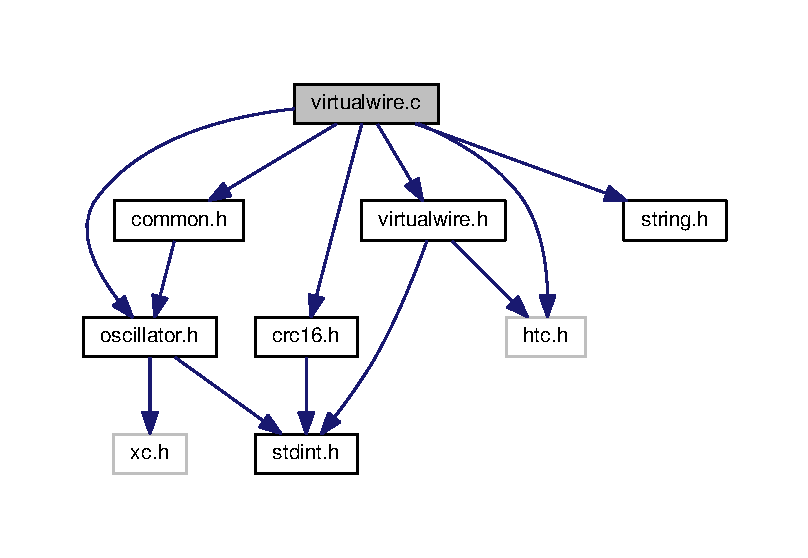
\includegraphics[width=350pt]{virtualwire_8c__incl}
\end{center}
\end{figure}
\subsection*{Macros}
\begin{DoxyCompactItemize}
\item 
\#define \hyperlink{virtualwire_8c_a4fb3d4b04fa0cd2d18d5f35c99a44bcf}{Tx\+Data}~P\+O\+R\+T\+Cbits.\+R\+C6
\item 
\#define \hyperlink{virtualwire_8c_af3b08f684c3b12f819c4c3d43146900a}{Rx\+Data}~P\+O\+R\+T\+Cbits.\+R\+C7
\item 
\#define \hyperlink{virtualwire_8c_a0cc5e5407f3ca16b7a0a7dd145a17b5e}{Tx\+Tris}~T\+R\+I\+S\+Cbits.\+T\+R\+I\+S\+C6
\item 
\#define \hyperlink{virtualwire_8c_aa430561cd375cc472e4c43f817f6b507}{Rx\+Tris}~T\+R\+I\+S\+Cbits.\+T\+R\+I\+S\+C7
\item 
\#define \hyperlink{virtualwire_8c_aba7d938851efb9ea95d05c45fc003e91}{O\+V\+E\+R\+S\+A\+M\+P\+L\+I\+N\+G}~8ul
\item 
\#define \hyperlink{virtualwire_8c_af48f8055714fb577ce1a7c496ab7aaa6}{V\+W\+\_\+\+R\+X\+\_\+\+R\+A\+M\+P\+\_\+\+L\+E\+N}~160
\begin{DoxyCompactList}\small\item\em The size of the receiver ramp. Ramp wraps modulu this number. \end{DoxyCompactList}\item 
\#define \hyperlink{virtualwire_8c_ad5a5c8919a669ce0121375f7bc08f376}{V\+W\+\_\+\+R\+X\+\_\+\+S\+A\+M\+P\+L\+E\+S\+\_\+\+P\+E\+R\+\_\+\+B\+I\+T}~8
\begin{DoxyCompactList}\small\item\em Number of samples per bit. \end{DoxyCompactList}\item 
\#define \hyperlink{virtualwire_8c_aa0cc20bc395fcefb080c0b7674623038}{V\+W\+\_\+\+R\+A\+M\+P\+\_\+\+I\+N\+C}~(\hyperlink{virtualwire_8c_af48f8055714fb577ce1a7c496ab7aaa6}{V\+W\+\_\+\+R\+X\+\_\+\+R\+A\+M\+P\+\_\+\+L\+E\+N}/\hyperlink{virtualwire_8c_ad5a5c8919a669ce0121375f7bc08f376}{V\+W\+\_\+\+R\+X\+\_\+\+S\+A\+M\+P\+L\+E\+S\+\_\+\+P\+E\+R\+\_\+\+B\+I\+T})
\begin{DoxyCompactList}\small\item\em Internal ramp adjustment parameter. \end{DoxyCompactList}\item 
\#define \hyperlink{virtualwire_8c_a8f592fa10bd1cd9aa3cde21e1b7b8f85}{V\+W\+\_\+\+R\+A\+M\+P\+\_\+\+T\+R\+A\+N\+S\+I\+T\+I\+O\+N}~\hyperlink{virtualwire_8c_af48f8055714fb577ce1a7c496ab7aaa6}{V\+W\+\_\+\+R\+X\+\_\+\+R\+A\+M\+P\+\_\+\+L\+E\+N}/2
\begin{DoxyCompactList}\small\item\em Internal ramp adjustment parameter. \end{DoxyCompactList}\item 
\#define \hyperlink{virtualwire_8c_ad6c091ae0ab196b5150a6de9ef868539}{V\+W\+\_\+\+R\+A\+M\+P\+\_\+\+A\+D\+J\+U\+S\+T}~9
\begin{DoxyCompactList}\small\item\em Internal ramp adjustment parameter. \end{DoxyCompactList}\item 
\#define \hyperlink{virtualwire_8c_aaac6e7f3bcf04ff6e6734abd80f7fc67}{V\+W\+\_\+\+R\+A\+M\+P\+\_\+\+I\+N\+C\+\_\+\+R\+E\+T\+A\+R\+D}~(\hyperlink{virtualwire_8c_aa0cc20bc395fcefb080c0b7674623038}{V\+W\+\_\+\+R\+A\+M\+P\+\_\+\+I\+N\+C}-\/\hyperlink{virtualwire_8c_ad6c091ae0ab196b5150a6de9ef868539}{V\+W\+\_\+\+R\+A\+M\+P\+\_\+\+A\+D\+J\+U\+S\+T})
\begin{DoxyCompactList}\small\item\em Internal ramp adjustment parameter. \end{DoxyCompactList}\item 
\#define \hyperlink{virtualwire_8c_a06c6a3d88ba1c8410bbbec928f1b1cac}{V\+W\+\_\+\+R\+A\+M\+P\+\_\+\+I\+N\+C\+\_\+\+A\+D\+V\+A\+N\+C\+E}~(\hyperlink{virtualwire_8c_aa0cc20bc395fcefb080c0b7674623038}{V\+W\+\_\+\+R\+A\+M\+P\+\_\+\+I\+N\+C}+\hyperlink{virtualwire_8c_ad6c091ae0ab196b5150a6de9ef868539}{V\+W\+\_\+\+R\+A\+M\+P\+\_\+\+A\+D\+J\+U\+S\+T})
\begin{DoxyCompactList}\small\item\em Internal ramp adjustment parameter. \end{DoxyCompactList}\item 
\#define \hyperlink{virtualwire_8c_a8457f2497e3ba191c30504d83bc275db}{V\+W\+\_\+\+H\+E\+A\+D\+E\+R\+\_\+\+L\+E\+N}~8
\item 
\#define \hyperlink{virtualwire_8c_a603f4fa1a2bb0c02a1c54a466e907f6e}{V\+W\+\_\+\+M\+A\+X\+\_\+\+P\+A\+Y\+L\+O\+A\+D}~\hyperlink{virtualwire_8h_a452f8c2d0db1bb9a2ca507642f396715}{V\+W\+\_\+\+M\+A\+X\+\_\+\+M\+E\+S\+S\+A\+G\+E\+\_\+\+L\+E\+N}-\/3
\end{DoxyCompactItemize}
\subsection*{Functions}
\begin{DoxyCompactItemize}
\item 
void \hyperlink{virtualwire_8c_a624514d01b56b031715326a9e659051b}{vw\+\_\+setup} (\hyperlink{stdint_8h_a06896e8c53f721507066c079052171f8}{uint32\+\_\+t} brate)
\item 
void \hyperlink{virtualwire_8c_ade1d3ba4e1422ee14f09bad1310793a7}{vw\+\_\+wait\+\_\+tx} (void)
\item 
void \hyperlink{virtualwire_8c_ae55855a5285218ca08d657a2a221a385}{vw\+\_\+tx\+\_\+stop} (void)
\item 
void \hyperlink{virtualwire_8c_a58fe5bfe18b5ba5ef6c6b27f47c2b18c}{vw\+\_\+tx\+\_\+start} (void)
\item 
bit \hyperlink{virtualwire_8c_adba805e998ddf1af21ef9b80c4a12a7e}{vw\+\_\+send} (const char $\ast$buf, \hyperlink{stdint_8h_aba7bc1797add20fe3efdf37ced1182c5}{uint8\+\_\+t} len)
\item 
\hyperlink{stdint_8h_a1f1825b69244eb3ad2c7165ddc99c956}{uint16\+\_\+t} \hyperlink{virtualwire_8c_aaf43bad86ec479208b4071c4a5816b6d}{vw\+\_\+crc} (\hyperlink{stdint_8h_aba7bc1797add20fe3efdf37ced1182c5}{uint8\+\_\+t} $\ast$ptr, \hyperlink{stdint_8h_aba7bc1797add20fe3efdf37ced1182c5}{uint8\+\_\+t} count)
\item 
\hyperlink{stdint_8h_aba7bc1797add20fe3efdf37ced1182c5}{uint8\+\_\+t} \hyperlink{virtualwire_8c_ace286b4c75ee0a2e05f1ba33dd767c24}{vw\+\_\+symbol\+\_\+6to4} (\hyperlink{stdint_8h_aba7bc1797add20fe3efdf37ced1182c5}{uint8\+\_\+t} symbol)
\item 
void \hyperlink{virtualwire_8c_a4ac2caf902c4059d06f22d78a1170b1f}{vw\+\_\+pll} (void)
\item 
bit \hyperlink{virtualwire_8c_a50bc13ae05d0e20edd48f31eb8805258}{vw\+\_\+have\+\_\+message} (void)
\item 
bit \hyperlink{virtualwire_8c_a885522cb1b1edd6a942b565c50b18b35}{vw\+\_\+recv} (\hyperlink{stdint_8h_aba7bc1797add20fe3efdf37ced1182c5}{uint8\+\_\+t} $\ast$buf, \hyperlink{stdint_8h_aba7bc1797add20fe3efdf37ced1182c5}{uint8\+\_\+t} $\ast$len)
\item 
void \hyperlink{virtualwire_8c_a6cb68e772da9c49f72b7131c03643f4d}{vw\+\_\+rx\+\_\+stop} (void)
\item 
void \hyperlink{virtualwire_8c_aa0720cfe48c78dfa436dafe65f1ddd12}{vw\+\_\+rx\+\_\+start} (void)
\item 
void \hyperlink{virtualwire_8c_aa0841d3f51ed4ac148448b4f3610ec89}{vw\+\_\+isr\+\_\+tmr0} (void)
\end{DoxyCompactItemize}
\subsection*{Variables}
\begin{DoxyCompactItemize}
\item 
const \hyperlink{stdint_8h_aba7bc1797add20fe3efdf37ced1182c5}{uint8\+\_\+t} \hyperlink{virtualwire_8c_ac818e046c1eebebadee93bd70f562e69}{symbols} \mbox{[}$\,$\mbox{]}
\item 
const \hyperlink{stdint_8h_aba7bc1797add20fe3efdf37ced1182c5}{uint8\+\_\+t} \hyperlink{virtualwire_8c_ae9e5cb0779456ff1b9626adc822757f9}{vw\+\_\+tx\+\_\+buf\+\_\+header} \mbox{[}\hyperlink{virtualwire_8c_a8457f2497e3ba191c30504d83bc275db}{V\+W\+\_\+\+H\+E\+A\+D\+E\+R\+\_\+\+L\+E\+N}\mbox{]} = \{0x2a, 0x2a, 0x2a, 0x2a, 0x2a, 0x2a, 0x38, 0x2c\}
\end{DoxyCompactItemize}


\subsection{Macro Definition Documentation}
\hypertarget{virtualwire_8c_aba7d938851efb9ea95d05c45fc003e91}{\index{virtualwire.\+c@{virtualwire.\+c}!O\+V\+E\+R\+S\+A\+M\+P\+L\+I\+N\+G@{O\+V\+E\+R\+S\+A\+M\+P\+L\+I\+N\+G}}
\index{O\+V\+E\+R\+S\+A\+M\+P\+L\+I\+N\+G@{O\+V\+E\+R\+S\+A\+M\+P\+L\+I\+N\+G}!virtualwire.\+c@{virtualwire.\+c}}
\subsubsection[{O\+V\+E\+R\+S\+A\+M\+P\+L\+I\+N\+G}]{\setlength{\rightskip}{0pt plus 5cm}\#define O\+V\+E\+R\+S\+A\+M\+P\+L\+I\+N\+G~8ul}}\label{virtualwire_8c_aba7d938851efb9ea95d05c45fc003e91}
\hypertarget{virtualwire_8c_af3b08f684c3b12f819c4c3d43146900a}{\index{virtualwire.\+c@{virtualwire.\+c}!Rx\+Data@{Rx\+Data}}
\index{Rx\+Data@{Rx\+Data}!virtualwire.\+c@{virtualwire.\+c}}
\subsubsection[{Rx\+Data}]{\setlength{\rightskip}{0pt plus 5cm}\#define Rx\+Data~P\+O\+R\+T\+Cbits.\+R\+C7}}\label{virtualwire_8c_af3b08f684c3b12f819c4c3d43146900a}
\hypertarget{virtualwire_8c_aa430561cd375cc472e4c43f817f6b507}{\index{virtualwire.\+c@{virtualwire.\+c}!Rx\+Tris@{Rx\+Tris}}
\index{Rx\+Tris@{Rx\+Tris}!virtualwire.\+c@{virtualwire.\+c}}
\subsubsection[{Rx\+Tris}]{\setlength{\rightskip}{0pt plus 5cm}\#define Rx\+Tris~T\+R\+I\+S\+Cbits.\+T\+R\+I\+S\+C7}}\label{virtualwire_8c_aa430561cd375cc472e4c43f817f6b507}
\hypertarget{virtualwire_8c_a4fb3d4b04fa0cd2d18d5f35c99a44bcf}{\index{virtualwire.\+c@{virtualwire.\+c}!Tx\+Data@{Tx\+Data}}
\index{Tx\+Data@{Tx\+Data}!virtualwire.\+c@{virtualwire.\+c}}
\subsubsection[{Tx\+Data}]{\setlength{\rightskip}{0pt plus 5cm}\#define Tx\+Data~P\+O\+R\+T\+Cbits.\+R\+C6}}\label{virtualwire_8c_a4fb3d4b04fa0cd2d18d5f35c99a44bcf}
\hypertarget{virtualwire_8c_a0cc5e5407f3ca16b7a0a7dd145a17b5e}{\index{virtualwire.\+c@{virtualwire.\+c}!Tx\+Tris@{Tx\+Tris}}
\index{Tx\+Tris@{Tx\+Tris}!virtualwire.\+c@{virtualwire.\+c}}
\subsubsection[{Tx\+Tris}]{\setlength{\rightskip}{0pt plus 5cm}\#define Tx\+Tris~T\+R\+I\+S\+Cbits.\+T\+R\+I\+S\+C6}}\label{virtualwire_8c_a0cc5e5407f3ca16b7a0a7dd145a17b5e}
\hypertarget{virtualwire_8c_a8457f2497e3ba191c30504d83bc275db}{\index{virtualwire.\+c@{virtualwire.\+c}!V\+W\+\_\+\+H\+E\+A\+D\+E\+R\+\_\+\+L\+E\+N@{V\+W\+\_\+\+H\+E\+A\+D\+E\+R\+\_\+\+L\+E\+N}}
\index{V\+W\+\_\+\+H\+E\+A\+D\+E\+R\+\_\+\+L\+E\+N@{V\+W\+\_\+\+H\+E\+A\+D\+E\+R\+\_\+\+L\+E\+N}!virtualwire.\+c@{virtualwire.\+c}}
\subsubsection[{V\+W\+\_\+\+H\+E\+A\+D\+E\+R\+\_\+\+L\+E\+N}]{\setlength{\rightskip}{0pt plus 5cm}\#define V\+W\+\_\+\+H\+E\+A\+D\+E\+R\+\_\+\+L\+E\+N~8}}\label{virtualwire_8c_a8457f2497e3ba191c30504d83bc275db}
\hypertarget{virtualwire_8c_a603f4fa1a2bb0c02a1c54a466e907f6e}{\index{virtualwire.\+c@{virtualwire.\+c}!V\+W\+\_\+\+M\+A\+X\+\_\+\+P\+A\+Y\+L\+O\+A\+D@{V\+W\+\_\+\+M\+A\+X\+\_\+\+P\+A\+Y\+L\+O\+A\+D}}
\index{V\+W\+\_\+\+M\+A\+X\+\_\+\+P\+A\+Y\+L\+O\+A\+D@{V\+W\+\_\+\+M\+A\+X\+\_\+\+P\+A\+Y\+L\+O\+A\+D}!virtualwire.\+c@{virtualwire.\+c}}
\subsubsection[{V\+W\+\_\+\+M\+A\+X\+\_\+\+P\+A\+Y\+L\+O\+A\+D}]{\setlength{\rightskip}{0pt plus 5cm}\#define V\+W\+\_\+\+M\+A\+X\+\_\+\+P\+A\+Y\+L\+O\+A\+D~{\bf V\+W\+\_\+\+M\+A\+X\+\_\+\+M\+E\+S\+S\+A\+G\+E\+\_\+\+L\+E\+N}-\/3}}\label{virtualwire_8c_a603f4fa1a2bb0c02a1c54a466e907f6e}
\hypertarget{virtualwire_8c_ad6c091ae0ab196b5150a6de9ef868539}{\index{virtualwire.\+c@{virtualwire.\+c}!V\+W\+\_\+\+R\+A\+M\+P\+\_\+\+A\+D\+J\+U\+S\+T@{V\+W\+\_\+\+R\+A\+M\+P\+\_\+\+A\+D\+J\+U\+S\+T}}
\index{V\+W\+\_\+\+R\+A\+M\+P\+\_\+\+A\+D\+J\+U\+S\+T@{V\+W\+\_\+\+R\+A\+M\+P\+\_\+\+A\+D\+J\+U\+S\+T}!virtualwire.\+c@{virtualwire.\+c}}
\subsubsection[{V\+W\+\_\+\+R\+A\+M\+P\+\_\+\+A\+D\+J\+U\+S\+T}]{\setlength{\rightskip}{0pt plus 5cm}\#define V\+W\+\_\+\+R\+A\+M\+P\+\_\+\+A\+D\+J\+U\+S\+T~9}}\label{virtualwire_8c_ad6c091ae0ab196b5150a6de9ef868539}


Internal ramp adjustment parameter. 

\hypertarget{virtualwire_8c_aa0cc20bc395fcefb080c0b7674623038}{\index{virtualwire.\+c@{virtualwire.\+c}!V\+W\+\_\+\+R\+A\+M\+P\+\_\+\+I\+N\+C@{V\+W\+\_\+\+R\+A\+M\+P\+\_\+\+I\+N\+C}}
\index{V\+W\+\_\+\+R\+A\+M\+P\+\_\+\+I\+N\+C@{V\+W\+\_\+\+R\+A\+M\+P\+\_\+\+I\+N\+C}!virtualwire.\+c@{virtualwire.\+c}}
\subsubsection[{V\+W\+\_\+\+R\+A\+M\+P\+\_\+\+I\+N\+C}]{\setlength{\rightskip}{0pt plus 5cm}\#define V\+W\+\_\+\+R\+A\+M\+P\+\_\+\+I\+N\+C~({\bf V\+W\+\_\+\+R\+X\+\_\+\+R\+A\+M\+P\+\_\+\+L\+E\+N}/{\bf V\+W\+\_\+\+R\+X\+\_\+\+S\+A\+M\+P\+L\+E\+S\+\_\+\+P\+E\+R\+\_\+\+B\+I\+T})}}\label{virtualwire_8c_aa0cc20bc395fcefb080c0b7674623038}


Internal ramp adjustment parameter. 

\hypertarget{virtualwire_8c_a06c6a3d88ba1c8410bbbec928f1b1cac}{\index{virtualwire.\+c@{virtualwire.\+c}!V\+W\+\_\+\+R\+A\+M\+P\+\_\+\+I\+N\+C\+\_\+\+A\+D\+V\+A\+N\+C\+E@{V\+W\+\_\+\+R\+A\+M\+P\+\_\+\+I\+N\+C\+\_\+\+A\+D\+V\+A\+N\+C\+E}}
\index{V\+W\+\_\+\+R\+A\+M\+P\+\_\+\+I\+N\+C\+\_\+\+A\+D\+V\+A\+N\+C\+E@{V\+W\+\_\+\+R\+A\+M\+P\+\_\+\+I\+N\+C\+\_\+\+A\+D\+V\+A\+N\+C\+E}!virtualwire.\+c@{virtualwire.\+c}}
\subsubsection[{V\+W\+\_\+\+R\+A\+M\+P\+\_\+\+I\+N\+C\+\_\+\+A\+D\+V\+A\+N\+C\+E}]{\setlength{\rightskip}{0pt plus 5cm}\#define V\+W\+\_\+\+R\+A\+M\+P\+\_\+\+I\+N\+C\+\_\+\+A\+D\+V\+A\+N\+C\+E~({\bf V\+W\+\_\+\+R\+A\+M\+P\+\_\+\+I\+N\+C}+{\bf V\+W\+\_\+\+R\+A\+M\+P\+\_\+\+A\+D\+J\+U\+S\+T})}}\label{virtualwire_8c_a06c6a3d88ba1c8410bbbec928f1b1cac}


Internal ramp adjustment parameter. 

\hypertarget{virtualwire_8c_aaac6e7f3bcf04ff6e6734abd80f7fc67}{\index{virtualwire.\+c@{virtualwire.\+c}!V\+W\+\_\+\+R\+A\+M\+P\+\_\+\+I\+N\+C\+\_\+\+R\+E\+T\+A\+R\+D@{V\+W\+\_\+\+R\+A\+M\+P\+\_\+\+I\+N\+C\+\_\+\+R\+E\+T\+A\+R\+D}}
\index{V\+W\+\_\+\+R\+A\+M\+P\+\_\+\+I\+N\+C\+\_\+\+R\+E\+T\+A\+R\+D@{V\+W\+\_\+\+R\+A\+M\+P\+\_\+\+I\+N\+C\+\_\+\+R\+E\+T\+A\+R\+D}!virtualwire.\+c@{virtualwire.\+c}}
\subsubsection[{V\+W\+\_\+\+R\+A\+M\+P\+\_\+\+I\+N\+C\+\_\+\+R\+E\+T\+A\+R\+D}]{\setlength{\rightskip}{0pt plus 5cm}\#define V\+W\+\_\+\+R\+A\+M\+P\+\_\+\+I\+N\+C\+\_\+\+R\+E\+T\+A\+R\+D~({\bf V\+W\+\_\+\+R\+A\+M\+P\+\_\+\+I\+N\+C}-\/{\bf V\+W\+\_\+\+R\+A\+M\+P\+\_\+\+A\+D\+J\+U\+S\+T})}}\label{virtualwire_8c_aaac6e7f3bcf04ff6e6734abd80f7fc67}


Internal ramp adjustment parameter. 

\hypertarget{virtualwire_8c_a8f592fa10bd1cd9aa3cde21e1b7b8f85}{\index{virtualwire.\+c@{virtualwire.\+c}!V\+W\+\_\+\+R\+A\+M\+P\+\_\+\+T\+R\+A\+N\+S\+I\+T\+I\+O\+N@{V\+W\+\_\+\+R\+A\+M\+P\+\_\+\+T\+R\+A\+N\+S\+I\+T\+I\+O\+N}}
\index{V\+W\+\_\+\+R\+A\+M\+P\+\_\+\+T\+R\+A\+N\+S\+I\+T\+I\+O\+N@{V\+W\+\_\+\+R\+A\+M\+P\+\_\+\+T\+R\+A\+N\+S\+I\+T\+I\+O\+N}!virtualwire.\+c@{virtualwire.\+c}}
\subsubsection[{V\+W\+\_\+\+R\+A\+M\+P\+\_\+\+T\+R\+A\+N\+S\+I\+T\+I\+O\+N}]{\setlength{\rightskip}{0pt plus 5cm}\#define V\+W\+\_\+\+R\+A\+M\+P\+\_\+\+T\+R\+A\+N\+S\+I\+T\+I\+O\+N~{\bf V\+W\+\_\+\+R\+X\+\_\+\+R\+A\+M\+P\+\_\+\+L\+E\+N}/2}}\label{virtualwire_8c_a8f592fa10bd1cd9aa3cde21e1b7b8f85}


Internal ramp adjustment parameter. 

\hypertarget{virtualwire_8c_af48f8055714fb577ce1a7c496ab7aaa6}{\index{virtualwire.\+c@{virtualwire.\+c}!V\+W\+\_\+\+R\+X\+\_\+\+R\+A\+M\+P\+\_\+\+L\+E\+N@{V\+W\+\_\+\+R\+X\+\_\+\+R\+A\+M\+P\+\_\+\+L\+E\+N}}
\index{V\+W\+\_\+\+R\+X\+\_\+\+R\+A\+M\+P\+\_\+\+L\+E\+N@{V\+W\+\_\+\+R\+X\+\_\+\+R\+A\+M\+P\+\_\+\+L\+E\+N}!virtualwire.\+c@{virtualwire.\+c}}
\subsubsection[{V\+W\+\_\+\+R\+X\+\_\+\+R\+A\+M\+P\+\_\+\+L\+E\+N}]{\setlength{\rightskip}{0pt plus 5cm}\#define V\+W\+\_\+\+R\+X\+\_\+\+R\+A\+M\+P\+\_\+\+L\+E\+N~160}}\label{virtualwire_8c_af48f8055714fb577ce1a7c496ab7aaa6}


The size of the receiver ramp. Ramp wraps modulu this number. 

\hypertarget{virtualwire_8c_ad5a5c8919a669ce0121375f7bc08f376}{\index{virtualwire.\+c@{virtualwire.\+c}!V\+W\+\_\+\+R\+X\+\_\+\+S\+A\+M\+P\+L\+E\+S\+\_\+\+P\+E\+R\+\_\+\+B\+I\+T@{V\+W\+\_\+\+R\+X\+\_\+\+S\+A\+M\+P\+L\+E\+S\+\_\+\+P\+E\+R\+\_\+\+B\+I\+T}}
\index{V\+W\+\_\+\+R\+X\+\_\+\+S\+A\+M\+P\+L\+E\+S\+\_\+\+P\+E\+R\+\_\+\+B\+I\+T@{V\+W\+\_\+\+R\+X\+\_\+\+S\+A\+M\+P\+L\+E\+S\+\_\+\+P\+E\+R\+\_\+\+B\+I\+T}!virtualwire.\+c@{virtualwire.\+c}}
\subsubsection[{V\+W\+\_\+\+R\+X\+\_\+\+S\+A\+M\+P\+L\+E\+S\+\_\+\+P\+E\+R\+\_\+\+B\+I\+T}]{\setlength{\rightskip}{0pt plus 5cm}\#define V\+W\+\_\+\+R\+X\+\_\+\+S\+A\+M\+P\+L\+E\+S\+\_\+\+P\+E\+R\+\_\+\+B\+I\+T~8}}\label{virtualwire_8c_ad5a5c8919a669ce0121375f7bc08f376}


Number of samples per bit. 



\subsection{Function Documentation}
\hypertarget{virtualwire_8c_aaf43bad86ec479208b4071c4a5816b6d}{\index{virtualwire.\+c@{virtualwire.\+c}!vw\+\_\+crc@{vw\+\_\+crc}}
\index{vw\+\_\+crc@{vw\+\_\+crc}!virtualwire.\+c@{virtualwire.\+c}}
\subsubsection[{vw\+\_\+crc}]{\setlength{\rightskip}{0pt plus 5cm}{\bf uint16\+\_\+t} vw\+\_\+crc (
\begin{DoxyParamCaption}
\item[{{\bf uint8\+\_\+t} $\ast$}]{ptr, }
\item[{{\bf uint8\+\_\+t}}]{count}
\end{DoxyParamCaption}
)}}\label{virtualwire_8c_aaf43bad86ec479208b4071c4a5816b6d}
\hypertarget{virtualwire_8c_a50bc13ae05d0e20edd48f31eb8805258}{\index{virtualwire.\+c@{virtualwire.\+c}!vw\+\_\+have\+\_\+message@{vw\+\_\+have\+\_\+message}}
\index{vw\+\_\+have\+\_\+message@{vw\+\_\+have\+\_\+message}!virtualwire.\+c@{virtualwire.\+c}}
\subsubsection[{vw\+\_\+have\+\_\+message}]{\setlength{\rightskip}{0pt plus 5cm}bit vw\+\_\+have\+\_\+message (
\begin{DoxyParamCaption}
\item[{void}]{}
\end{DoxyParamCaption}
)}}\label{virtualwire_8c_a50bc13ae05d0e20edd48f31eb8805258}
\hypertarget{virtualwire_8c_aa0841d3f51ed4ac148448b4f3610ec89}{\index{virtualwire.\+c@{virtualwire.\+c}!vw\+\_\+isr\+\_\+tmr0@{vw\+\_\+isr\+\_\+tmr0}}
\index{vw\+\_\+isr\+\_\+tmr0@{vw\+\_\+isr\+\_\+tmr0}!virtualwire.\+c@{virtualwire.\+c}}
\subsubsection[{vw\+\_\+isr\+\_\+tmr0}]{\setlength{\rightskip}{0pt plus 5cm}void vw\+\_\+isr\+\_\+tmr0 (
\begin{DoxyParamCaption}
\item[{void}]{}
\end{DoxyParamCaption}
)}}\label{virtualwire_8c_aa0841d3f51ed4ac148448b4f3610ec89}
\hypertarget{virtualwire_8c_a4ac2caf902c4059d06f22d78a1170b1f}{\index{virtualwire.\+c@{virtualwire.\+c}!vw\+\_\+pll@{vw\+\_\+pll}}
\index{vw\+\_\+pll@{vw\+\_\+pll}!virtualwire.\+c@{virtualwire.\+c}}
\subsubsection[{vw\+\_\+pll}]{\setlength{\rightskip}{0pt plus 5cm}void vw\+\_\+pll (
\begin{DoxyParamCaption}
\item[{void}]{}
\end{DoxyParamCaption}
)}}\label{virtualwire_8c_a4ac2caf902c4059d06f22d78a1170b1f}
\hypertarget{virtualwire_8c_a885522cb1b1edd6a942b565c50b18b35}{\index{virtualwire.\+c@{virtualwire.\+c}!vw\+\_\+recv@{vw\+\_\+recv}}
\index{vw\+\_\+recv@{vw\+\_\+recv}!virtualwire.\+c@{virtualwire.\+c}}
\subsubsection[{vw\+\_\+recv}]{\setlength{\rightskip}{0pt plus 5cm}bit vw\+\_\+recv (
\begin{DoxyParamCaption}
\item[{{\bf uint8\+\_\+t} $\ast$}]{buf, }
\item[{{\bf uint8\+\_\+t} $\ast$}]{len}
\end{DoxyParamCaption}
)}}\label{virtualwire_8c_a885522cb1b1edd6a942b565c50b18b35}
\hypertarget{virtualwire_8c_aa0720cfe48c78dfa436dafe65f1ddd12}{\index{virtualwire.\+c@{virtualwire.\+c}!vw\+\_\+rx\+\_\+start@{vw\+\_\+rx\+\_\+start}}
\index{vw\+\_\+rx\+\_\+start@{vw\+\_\+rx\+\_\+start}!virtualwire.\+c@{virtualwire.\+c}}
\subsubsection[{vw\+\_\+rx\+\_\+start}]{\setlength{\rightskip}{0pt plus 5cm}void vw\+\_\+rx\+\_\+start (
\begin{DoxyParamCaption}
\item[{void}]{}
\end{DoxyParamCaption}
)}}\label{virtualwire_8c_aa0720cfe48c78dfa436dafe65f1ddd12}
\hypertarget{virtualwire_8c_a6cb68e772da9c49f72b7131c03643f4d}{\index{virtualwire.\+c@{virtualwire.\+c}!vw\+\_\+rx\+\_\+stop@{vw\+\_\+rx\+\_\+stop}}
\index{vw\+\_\+rx\+\_\+stop@{vw\+\_\+rx\+\_\+stop}!virtualwire.\+c@{virtualwire.\+c}}
\subsubsection[{vw\+\_\+rx\+\_\+stop}]{\setlength{\rightskip}{0pt plus 5cm}void vw\+\_\+rx\+\_\+stop (
\begin{DoxyParamCaption}
\item[{void}]{}
\end{DoxyParamCaption}
)}}\label{virtualwire_8c_a6cb68e772da9c49f72b7131c03643f4d}
\hypertarget{virtualwire_8c_adba805e998ddf1af21ef9b80c4a12a7e}{\index{virtualwire.\+c@{virtualwire.\+c}!vw\+\_\+send@{vw\+\_\+send}}
\index{vw\+\_\+send@{vw\+\_\+send}!virtualwire.\+c@{virtualwire.\+c}}
\subsubsection[{vw\+\_\+send}]{\setlength{\rightskip}{0pt plus 5cm}bit vw\+\_\+send (
\begin{DoxyParamCaption}
\item[{const char $\ast$}]{buf, }
\item[{{\bf uint8\+\_\+t}}]{len}
\end{DoxyParamCaption}
)}}\label{virtualwire_8c_adba805e998ddf1af21ef9b80c4a12a7e}
\hypertarget{virtualwire_8c_a624514d01b56b031715326a9e659051b}{\index{virtualwire.\+c@{virtualwire.\+c}!vw\+\_\+setup@{vw\+\_\+setup}}
\index{vw\+\_\+setup@{vw\+\_\+setup}!virtualwire.\+c@{virtualwire.\+c}}
\subsubsection[{vw\+\_\+setup}]{\setlength{\rightskip}{0pt plus 5cm}void vw\+\_\+setup (
\begin{DoxyParamCaption}
\item[{{\bf uint32\+\_\+t}}]{brate}
\end{DoxyParamCaption}
)}}\label{virtualwire_8c_a624514d01b56b031715326a9e659051b}
\hypertarget{virtualwire_8c_ace286b4c75ee0a2e05f1ba33dd767c24}{\index{virtualwire.\+c@{virtualwire.\+c}!vw\+\_\+symbol\+\_\+6to4@{vw\+\_\+symbol\+\_\+6to4}}
\index{vw\+\_\+symbol\+\_\+6to4@{vw\+\_\+symbol\+\_\+6to4}!virtualwire.\+c@{virtualwire.\+c}}
\subsubsection[{vw\+\_\+symbol\+\_\+6to4}]{\setlength{\rightskip}{0pt plus 5cm}{\bf uint8\+\_\+t} vw\+\_\+symbol\+\_\+6to4 (
\begin{DoxyParamCaption}
\item[{{\bf uint8\+\_\+t}}]{symbol}
\end{DoxyParamCaption}
)}}\label{virtualwire_8c_ace286b4c75ee0a2e05f1ba33dd767c24}
\hypertarget{virtualwire_8c_a58fe5bfe18b5ba5ef6c6b27f47c2b18c}{\index{virtualwire.\+c@{virtualwire.\+c}!vw\+\_\+tx\+\_\+start@{vw\+\_\+tx\+\_\+start}}
\index{vw\+\_\+tx\+\_\+start@{vw\+\_\+tx\+\_\+start}!virtualwire.\+c@{virtualwire.\+c}}
\subsubsection[{vw\+\_\+tx\+\_\+start}]{\setlength{\rightskip}{0pt plus 5cm}void vw\+\_\+tx\+\_\+start (
\begin{DoxyParamCaption}
\item[{void}]{}
\end{DoxyParamCaption}
)}}\label{virtualwire_8c_a58fe5bfe18b5ba5ef6c6b27f47c2b18c}
\hypertarget{virtualwire_8c_ae55855a5285218ca08d657a2a221a385}{\index{virtualwire.\+c@{virtualwire.\+c}!vw\+\_\+tx\+\_\+stop@{vw\+\_\+tx\+\_\+stop}}
\index{vw\+\_\+tx\+\_\+stop@{vw\+\_\+tx\+\_\+stop}!virtualwire.\+c@{virtualwire.\+c}}
\subsubsection[{vw\+\_\+tx\+\_\+stop}]{\setlength{\rightskip}{0pt plus 5cm}void vw\+\_\+tx\+\_\+stop (
\begin{DoxyParamCaption}
\item[{void}]{}
\end{DoxyParamCaption}
)}}\label{virtualwire_8c_ae55855a5285218ca08d657a2a221a385}
\hypertarget{virtualwire_8c_ade1d3ba4e1422ee14f09bad1310793a7}{\index{virtualwire.\+c@{virtualwire.\+c}!vw\+\_\+wait\+\_\+tx@{vw\+\_\+wait\+\_\+tx}}
\index{vw\+\_\+wait\+\_\+tx@{vw\+\_\+wait\+\_\+tx}!virtualwire.\+c@{virtualwire.\+c}}
\subsubsection[{vw\+\_\+wait\+\_\+tx}]{\setlength{\rightskip}{0pt plus 5cm}void vw\+\_\+wait\+\_\+tx (
\begin{DoxyParamCaption}
\item[{void}]{}
\end{DoxyParamCaption}
)}}\label{virtualwire_8c_ade1d3ba4e1422ee14f09bad1310793a7}


\subsection{Variable Documentation}
\hypertarget{virtualwire_8c_ac818e046c1eebebadee93bd70f562e69}{\index{virtualwire.\+c@{virtualwire.\+c}!symbols@{symbols}}
\index{symbols@{symbols}!virtualwire.\+c@{virtualwire.\+c}}
\subsubsection[{symbols}]{\setlength{\rightskip}{0pt plus 5cm}const {\bf uint8\+\_\+t} symbols\mbox{[}$\,$\mbox{]}}}\label{virtualwire_8c_ac818e046c1eebebadee93bd70f562e69}
{\bfseries Initial value\+:}
\begin{DoxyCode}
= \{
    0xd, 0xe, 0x13, 0x15, 0x16, 0x19, 0x1a, 0x1c,
    0x23, 0x25, 0x26, 0x29, 0x2a, 0x2c, 0x32, 0x34
\}
\end{DoxyCode}
\hypertarget{virtualwire_8c_ae9e5cb0779456ff1b9626adc822757f9}{\index{virtualwire.\+c@{virtualwire.\+c}!vw\+\_\+tx\+\_\+buf\+\_\+header@{vw\+\_\+tx\+\_\+buf\+\_\+header}}
\index{vw\+\_\+tx\+\_\+buf\+\_\+header@{vw\+\_\+tx\+\_\+buf\+\_\+header}!virtualwire.\+c@{virtualwire.\+c}}
\subsubsection[{vw\+\_\+tx\+\_\+buf\+\_\+header}]{\setlength{\rightskip}{0pt plus 5cm}const {\bf uint8\+\_\+t} vw\+\_\+tx\+\_\+buf\+\_\+header\mbox{[}{\bf V\+W\+\_\+\+H\+E\+A\+D\+E\+R\+\_\+\+L\+E\+N}\mbox{]} = \{0x2a, 0x2a, 0x2a, 0x2a, 0x2a, 0x2a, 0x38, 0x2c\}}}\label{virtualwire_8c_ae9e5cb0779456ff1b9626adc822757f9}

\hypertarget{virtualwire_8h}{\section{virtualwire.\+h File Reference}
\label{virtualwire_8h}\index{virtualwire.\+h@{virtualwire.\+h}}
}
{\ttfamily \#include $<$htc.\+h$>$}\\*
{\ttfamily \#include \char`\"{}stdint.\+h\char`\"{}}\\*
Include dependency graph for virtualwire.\+h\+:\nopagebreak
\begin{figure}[H]
\begin{center}
\leavevmode
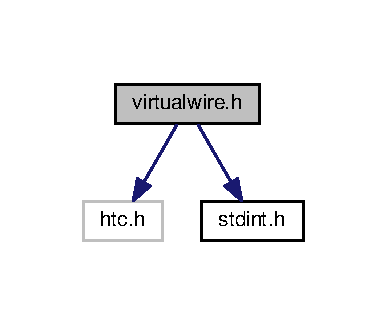
\includegraphics[width=185pt]{virtualwire_8h__incl}
\end{center}
\end{figure}
This graph shows which files directly or indirectly include this file\+:\nopagebreak
\begin{figure}[H]
\begin{center}
\leavevmode
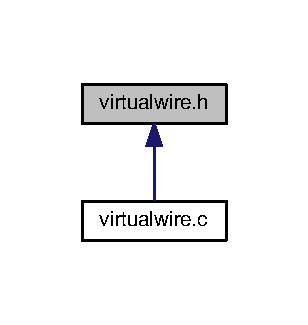
\includegraphics[width=148pt]{virtualwire_8h__dep__incl}
\end{center}
\end{figure}
\subsection*{Macros}
\begin{DoxyCompactItemize}
\item 
\#define \hyperlink{virtualwire_8h_a452f8c2d0db1bb9a2ca507642f396715}{V\+W\+\_\+\+M\+A\+X\+\_\+\+M\+E\+S\+S\+A\+G\+E\+\_\+\+L\+E\+N}~24
\end{DoxyCompactItemize}
\subsection*{Functions}
\begin{DoxyCompactItemize}
\item 
void \hyperlink{virtualwire_8h_a624514d01b56b031715326a9e659051b}{vw\+\_\+setup} (\hyperlink{stdint_8h_a06896e8c53f721507066c079052171f8}{uint32\+\_\+t} brate)
\item 
bit \hyperlink{virtualwire_8h_adba805e998ddf1af21ef9b80c4a12a7e}{vw\+\_\+send} (const char $\ast$buf, \hyperlink{stdint_8h_aba7bc1797add20fe3efdf37ced1182c5}{uint8\+\_\+t} len)
\item 
void \hyperlink{virtualwire_8h_ade1d3ba4e1422ee14f09bad1310793a7}{vw\+\_\+wait\+\_\+tx} (void)
\item 
bit \hyperlink{virtualwire_8h_a50bc13ae05d0e20edd48f31eb8805258}{vw\+\_\+have\+\_\+message} (void)
\item 
bit \hyperlink{virtualwire_8h_a885522cb1b1edd6a942b565c50b18b35}{vw\+\_\+recv} (\hyperlink{stdint_8h_aba7bc1797add20fe3efdf37ced1182c5}{uint8\+\_\+t} $\ast$buf, \hyperlink{stdint_8h_aba7bc1797add20fe3efdf37ced1182c5}{uint8\+\_\+t} $\ast$len)
\item 
void \hyperlink{virtualwire_8h_a6cb68e772da9c49f72b7131c03643f4d}{vw\+\_\+rx\+\_\+stop} (void)
\item 
void \hyperlink{virtualwire_8h_aa0720cfe48c78dfa436dafe65f1ddd12}{vw\+\_\+rx\+\_\+start} (void)
\item 
void \hyperlink{virtualwire_8h_aa0841d3f51ed4ac148448b4f3610ec89}{vw\+\_\+isr\+\_\+tmr0} (void)
\end{DoxyCompactItemize}


\subsection{Macro Definition Documentation}
\hypertarget{virtualwire_8h_a452f8c2d0db1bb9a2ca507642f396715}{\index{virtualwire.\+h@{virtualwire.\+h}!V\+W\+\_\+\+M\+A\+X\+\_\+\+M\+E\+S\+S\+A\+G\+E\+\_\+\+L\+E\+N@{V\+W\+\_\+\+M\+A\+X\+\_\+\+M\+E\+S\+S\+A\+G\+E\+\_\+\+L\+E\+N}}
\index{V\+W\+\_\+\+M\+A\+X\+\_\+\+M\+E\+S\+S\+A\+G\+E\+\_\+\+L\+E\+N@{V\+W\+\_\+\+M\+A\+X\+\_\+\+M\+E\+S\+S\+A\+G\+E\+\_\+\+L\+E\+N}!virtualwire.\+h@{virtualwire.\+h}}
\subsubsection[{V\+W\+\_\+\+M\+A\+X\+\_\+\+M\+E\+S\+S\+A\+G\+E\+\_\+\+L\+E\+N}]{\setlength{\rightskip}{0pt plus 5cm}\#define V\+W\+\_\+\+M\+A\+X\+\_\+\+M\+E\+S\+S\+A\+G\+E\+\_\+\+L\+E\+N~24}}\label{virtualwire_8h_a452f8c2d0db1bb9a2ca507642f396715}


\subsection{Function Documentation}
\hypertarget{virtualwire_8h_a50bc13ae05d0e20edd48f31eb8805258}{\index{virtualwire.\+h@{virtualwire.\+h}!vw\+\_\+have\+\_\+message@{vw\+\_\+have\+\_\+message}}
\index{vw\+\_\+have\+\_\+message@{vw\+\_\+have\+\_\+message}!virtualwire.\+h@{virtualwire.\+h}}
\subsubsection[{vw\+\_\+have\+\_\+message}]{\setlength{\rightskip}{0pt plus 5cm}bit vw\+\_\+have\+\_\+message (
\begin{DoxyParamCaption}
\item[{void}]{}
\end{DoxyParamCaption}
)}}\label{virtualwire_8h_a50bc13ae05d0e20edd48f31eb8805258}
\hypertarget{virtualwire_8h_aa0841d3f51ed4ac148448b4f3610ec89}{\index{virtualwire.\+h@{virtualwire.\+h}!vw\+\_\+isr\+\_\+tmr0@{vw\+\_\+isr\+\_\+tmr0}}
\index{vw\+\_\+isr\+\_\+tmr0@{vw\+\_\+isr\+\_\+tmr0}!virtualwire.\+h@{virtualwire.\+h}}
\subsubsection[{vw\+\_\+isr\+\_\+tmr0}]{\setlength{\rightskip}{0pt plus 5cm}void vw\+\_\+isr\+\_\+tmr0 (
\begin{DoxyParamCaption}
\item[{void}]{}
\end{DoxyParamCaption}
)}}\label{virtualwire_8h_aa0841d3f51ed4ac148448b4f3610ec89}
\hypertarget{virtualwire_8h_a885522cb1b1edd6a942b565c50b18b35}{\index{virtualwire.\+h@{virtualwire.\+h}!vw\+\_\+recv@{vw\+\_\+recv}}
\index{vw\+\_\+recv@{vw\+\_\+recv}!virtualwire.\+h@{virtualwire.\+h}}
\subsubsection[{vw\+\_\+recv}]{\setlength{\rightskip}{0pt plus 5cm}bit vw\+\_\+recv (
\begin{DoxyParamCaption}
\item[{{\bf uint8\+\_\+t} $\ast$}]{buf, }
\item[{{\bf uint8\+\_\+t} $\ast$}]{len}
\end{DoxyParamCaption}
)}}\label{virtualwire_8h_a885522cb1b1edd6a942b565c50b18b35}
\hypertarget{virtualwire_8h_aa0720cfe48c78dfa436dafe65f1ddd12}{\index{virtualwire.\+h@{virtualwire.\+h}!vw\+\_\+rx\+\_\+start@{vw\+\_\+rx\+\_\+start}}
\index{vw\+\_\+rx\+\_\+start@{vw\+\_\+rx\+\_\+start}!virtualwire.\+h@{virtualwire.\+h}}
\subsubsection[{vw\+\_\+rx\+\_\+start}]{\setlength{\rightskip}{0pt plus 5cm}void vw\+\_\+rx\+\_\+start (
\begin{DoxyParamCaption}
\item[{void}]{}
\end{DoxyParamCaption}
)}}\label{virtualwire_8h_aa0720cfe48c78dfa436dafe65f1ddd12}
\hypertarget{virtualwire_8h_a6cb68e772da9c49f72b7131c03643f4d}{\index{virtualwire.\+h@{virtualwire.\+h}!vw\+\_\+rx\+\_\+stop@{vw\+\_\+rx\+\_\+stop}}
\index{vw\+\_\+rx\+\_\+stop@{vw\+\_\+rx\+\_\+stop}!virtualwire.\+h@{virtualwire.\+h}}
\subsubsection[{vw\+\_\+rx\+\_\+stop}]{\setlength{\rightskip}{0pt plus 5cm}void vw\+\_\+rx\+\_\+stop (
\begin{DoxyParamCaption}
\item[{void}]{}
\end{DoxyParamCaption}
)}}\label{virtualwire_8h_a6cb68e772da9c49f72b7131c03643f4d}
\hypertarget{virtualwire_8h_adba805e998ddf1af21ef9b80c4a12a7e}{\index{virtualwire.\+h@{virtualwire.\+h}!vw\+\_\+send@{vw\+\_\+send}}
\index{vw\+\_\+send@{vw\+\_\+send}!virtualwire.\+h@{virtualwire.\+h}}
\subsubsection[{vw\+\_\+send}]{\setlength{\rightskip}{0pt plus 5cm}bit vw\+\_\+send (
\begin{DoxyParamCaption}
\item[{const char $\ast$}]{buf, }
\item[{{\bf uint8\+\_\+t}}]{len}
\end{DoxyParamCaption}
)}}\label{virtualwire_8h_adba805e998ddf1af21ef9b80c4a12a7e}
\hypertarget{virtualwire_8h_a624514d01b56b031715326a9e659051b}{\index{virtualwire.\+h@{virtualwire.\+h}!vw\+\_\+setup@{vw\+\_\+setup}}
\index{vw\+\_\+setup@{vw\+\_\+setup}!virtualwire.\+h@{virtualwire.\+h}}
\subsubsection[{vw\+\_\+setup}]{\setlength{\rightskip}{0pt plus 5cm}void vw\+\_\+setup (
\begin{DoxyParamCaption}
\item[{{\bf uint32\+\_\+t}}]{brate}
\end{DoxyParamCaption}
)}}\label{virtualwire_8h_a624514d01b56b031715326a9e659051b}
\hypertarget{virtualwire_8h_ade1d3ba4e1422ee14f09bad1310793a7}{\index{virtualwire.\+h@{virtualwire.\+h}!vw\+\_\+wait\+\_\+tx@{vw\+\_\+wait\+\_\+tx}}
\index{vw\+\_\+wait\+\_\+tx@{vw\+\_\+wait\+\_\+tx}!virtualwire.\+h@{virtualwire.\+h}}
\subsubsection[{vw\+\_\+wait\+\_\+tx}]{\setlength{\rightskip}{0pt plus 5cm}void vw\+\_\+wait\+\_\+tx (
\begin{DoxyParamCaption}
\item[{void}]{}
\end{DoxyParamCaption}
)}}\label{virtualwire_8h_ade1d3ba4e1422ee14f09bad1310793a7}

%--- End generated contents ---

% Index
\newpage
\phantomsection
\addcontentsline{toc}{chapter}{Index}
\printindex

\end{document}
